\documentclass[
	12pt,
	a4paper,
	DIVcalc,
	titlepage,
	twoside,
	liststotoc,
	bibtotocnumbered
]{scrbook}

%\usepackage[parfill]{parskip}    % Activate to begin paragraphs with an empty line rather than an indent
\usepackage[utf8]{inputenc}     %% dt. Umlaute mit utf-8, 
\usepackage[ngerman]{babel}
\usepackage{amsmath}
\usepackage{amsfonts}
\usepackage{amssymb}
\usepackage{graphicx}
\usepackage{algorithmic}
\algsetup{indent=1.7em}
\usepackage{natbib}
%\bibpunct{(}{)}{;}{a}{}{,} % to follow the A&A style

\usepackage[
	automark,		% Kapitelangaben in Kopfzeile automatisch erstellen
        headsepline,		% Trennlinie unter Kopfzeile
%        footsepline,
	ilines			% Trennlinie linksbündig ausrichten
]{scrpage2}
\pagestyle{scrheadings}

\usepackage[a4paper, bookmarks, colorlinks]{hyperref}	%%farbige Hyperlinks 
\hypersetup{%
	pdfkeywords = {},
	linkcolor = black,
	urlcolor = black,
	menucolor=black,
	citecolor = black,
	pagecolor=black,
	bookmarksopen = true, 
	bookmarksnumbered = true,
	pdfpagemode = {UseNone}, % UseNone, UseThumbs,UseOutlines, FullScreen
	pdfstartview = {} % ohne (nicht None), Fit, FitB
	%pdfcreator = {Adobe-Acrobat-Distiller},
	%pdfproducer = {LaTeX with hyperref and thumbpdf}
}

\begin{document}

\frontmatter
	\titlehead{Christian--Albrechts--Universit"at zu Kiel\\ Institut f"ur Theoretische Physik und Astrophysik}
	\subject{Diplomarbeit}
	\title{L"osung des Strahlungstransportproblems in Pfadintegralform mit effizienten Monte--Carlo--Verfahren}
	\author{vorgelegt von Thies Heidecke\\(theidecke@astrophysik.uni-kiel.de)}
	\publishers{betreut durch Prof. Dr. Sebastian Wolf}
	\date{Version vom \today}
	\maketitle
	% standard-titelblatt verf"ugbar?

	\tableofcontents	%%Inhaltsverzeichnis
	%\listoffigures	%%Abbildungsverzeichnis
	%\listoftables		%%Tabellenverzeichnis

	\newcommand{\location}[1]{\mathbf{#1}}
	\newcommand{\scatter}[1]{\overset{#1}{\leftrightsquigarrow}}
	\newcommand{\normalized}[1]{\frac{#1}{||#1||}}

\mainmatter
		\chapter{Einleitung}
	\section{Motivation}
	Menschen sind schon immer fasziniert von der Frage nach ihrer eigenen Herkunft und des Universums in dem sie Leben. Eine Facette dieser Frage ist der Wunsch, ein besseres Verständnis des kosmischen Zyklus von der Entstehung und dem Vergehen von Sternen zu erlangen. Dieses Thema ist insbesondere deshalb interessant, weil mit ihm die Entstehung von Planetensystemen verknüpft ist und es somit unsere eigene Herkunft berührt.
	
	In der Astrophysik lassen sich dabei zwei Wege einschlagen um sich diesem Ver\-ständ\-nis zu nähern. Der eine Weg führt über die Beobachtung der Sternentstehungsgebiete am Himmel, in denen nebeneinander verschiedene Entwicklungsstadien der Sternentstehung von Molekülwolken über Globulen, junge stellare Objekte (YSOs) mit protoplanetarer Scheibe, Vorhauptreihensterne und schließlich Hauptreihensterne beobachtet werden können.
	%\begin{wrapfigure}{l}{0.382\textwidth}
	%	\centering
	%	\vspace{-1em}
	%	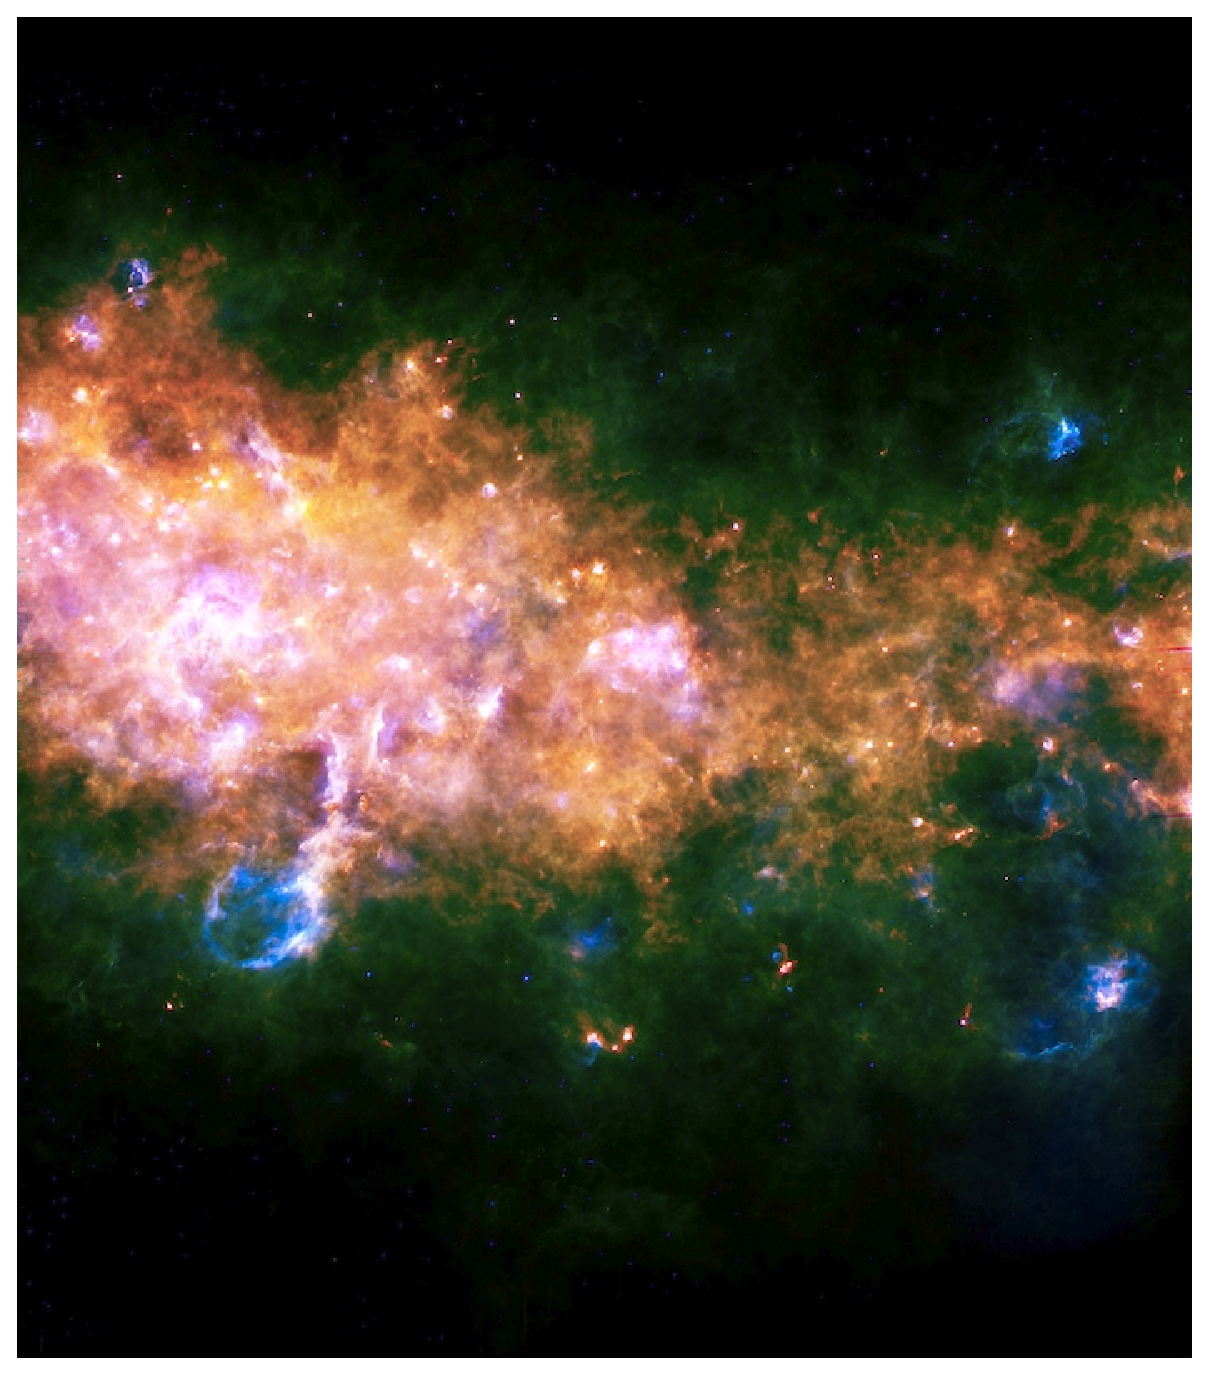
\includegraphics[width=0.382\textwidth]{Stellar_Gestation_and_Birth_in_the_Milky_Way.eps}
	%	\caption{Stern\-ent\-steh\-ungs\-ge\-biet im Ad\-ler\-ne\-bel. Auf\-ge\-nom\-men mit Her\-schel bei 70, 160 und 250$\mu$m im Dezember 2009.}
		% ($18^\text{h}46^\text{m}5.22^\text{s}$ / $+2^\circ 36'32.88"$)
	%	\vspace{-2em}
	%	\label{fig:starformingregion}
	%\end{wrapfigure}
	Auf den verschiedenen Beobachtungen lassen sich empirisch Theorien der Stern- und Planetenentstehung gründen. Der andere Weg führt von etablierten allgemeinen Theorien ausgehend über mathematische Herleitungen oder ``first--principles''--Simulationen zu Vorhersagen oder dem Nachvollzug der verschiedenen Phasen der Stern- und Planetenentstehung. Beide Wege sind nicht unabhängig voneinander sondern bilden vielmehr Abschnitte auf einem spiralförmigen Weg auf dem sich Empirie und Theorie abwechseln und durch Induktion und Deduktion gegenseitig eine bessere Ausgangslage schaffen.
	
	Im Bereich protoplanetarer Scheiben bildet Strahlungstransport den Teil der Theorie, der Vorhersagen über das Verhalten von Licht in einer vorgegebenen Anordnung von Materie macht. Strahlungstransport ist im Bereich protostellarer Scheiben somit einerseits wichtig für ein vollständiges Modell ihres Aufbaus, und andererseits wichtig, um ihr Aussehen vorherzusagen. Eine Simulation des Strahlungstransports erlaubt den Vergleich von Bildern aus Scheibenmodellen und mithilfe von Teleskopen aufgenommener Bilder und stellt somit das direkte Bindeglied zwischen Theorie und Beobachtung dar.
	
	Wir leben dabei in einer spannenden Zeit, in der die aktuelle und kommende Generation von Großteleskopen auf der Erde und im Weltraum detailreichere Daten von protostellaren Scheiben aufnehmen als je zuvor. Dies stellt auch höhere Anforderungen an Strahlungstransportsimulationen, von denen feinere und genauere Bilder und Spektren gebraucht werden um beim Vergleich mit Beobachtungsdaten von Nutzen zu sein.
	
	Dabei stellt sich häufig nicht das Problem, das Aussehen einer vorgegebenen Scheibenkonfiguration zu simulieren, sondern das inverse Problem, aus gegebenen Beobachtungsdaten unter physikalischen Nebenbedingungen die wahrscheinlichste Materieanordnung zu finden um die Beobachtung zu erklären. Das direkte Lösen dieses Problems ist i.A. nicht möglich. Daher ist der praktisch gegangene Ausweg das mehr oder weniger intelligente Raten von möglichst passenden Scheibenkonfigurationen, die nach einer Strahlungstransportsimulation mit den Beobachtungsdaten verglichen werden können. In dieser Situation ist eine effiziente Simulation umso nützlicher und u.U. entscheidend für den Unterschied zwischen dem Raten eines spezifischen Modells aufgrund einiger weniger Modellrechnungen und einer abdeckenden, statistisch signifikanten Schätzung der Modellparameter.
	
	Daher sollen in dieser Arbeit neue Ansätze zur effizienten Lösung des Strahlungstransportproblems vorgestellt, erprobt und diskutiert werden.
	
	\section{Ziele der Arbeit}
	In dieser Arbeit wird eine Pfadintegraldarstellung der Lösung des Strahlungstransportgleichung hergeleitet, sowie dessen Nutzen für Monte--Carlo--Verfahren zur Lösung des Strahlungstransportproblems theoretisch und praktisch in Form eines Computerprogrammes gezeigt.
	
	\section{Übersicht}
	Wir fangen in Kapitel 2 mit einer Einführung des Strahlungstransportproblems über ein allgemeines Teilchentransportproblem an, welches wir anschließend durch Spezialisierung der Teilchen auf Photonen auf die klassische Strahlungstransportgleichung zurückführen. Außerdem stellen wir einen allgemeinen Formalismus für Messungen des Strahlungsfeldes vor.
	
	In Kapitel 3 überführen wir die klassische Strahlungstransportgleichung über den Umweg einer Integraldarstellung in eine Operatorform, in der das Problem anschaulich und formal leicht lösbar ist. Die gewonnene Lösung stellen wir dann als Integral über den Raum aller möglichen Lichtpfade dar.
	
	In Kapitel 4 beschäftigen wir uns mit dem Problem der numerischen Integration und den Vor- und Nachteilen der Monte--Carlo--Integration im Vergleich zu klassischen numerischen Quadraturverfahren.
	
	In Kapitel 5 stellen wir ein weiteres Monte--Carlo--Verfahren vor, mit dem sich aus beliebigen statistischen Verteilungen Stichproben erzeugen lassen und erklären, wozu dies im Zusammenhang mit der Lösung des Strahlungstransportproblems nützlich ist.
	
	In Kapitel 6 führen wir die bis dahin behandelten Themen Strahlungstransport und Monte--Carlo--Verfahren zusammen. Wir zeigen, wie sich die in Kapitel 3 hergeleitete Pfadintegrallösung des Strahlungstransportproblems als Integrationsproblem darstellen lässt, auf die unsere Monte--Carlo--Integrationsverfahren aus Kapitel 4 direkt anwendbar sind. Ergänzend dazu stellen wir Methoden vor, um die Konvergenz der Integration durch eine gehäuftere Berücksichtigung der für den Strahlungstransport wesentlichen Pfade zu verbessern.
	
	In Kapitel 7 stellen wir das Programm \pirate vor, in dem viele der vorgestellten Ideen implementiert sind.
	
	In Kapitel 8 vergleichen wir dann die Ergebnisse und die Geschwindigkeit von \pirate mit dem Referenzprogramm \texttt{MC3D}.
	
	Schließlich fassen wir in Kapitel 9 die Arbeit zusammen und geben einen Ausblick, wie die vorgestellten Ideen und das Programm \pirate weiterentwickelt und eingesetzt werden können.
	
	\vfill
	\pagebreak
	\section{Nomenklatur}\label{subsec:nomenklatur}
	Im folgenden Text werden die in Tabelle \ref{tab:nomenklatur} angegebenen Schreibweisen benutzt.

	\begin{table}
		\caption{Nomenklatur}
		\begin{center}
		\begin{tabular}{rll}
			Schreibweise & Bedeutung & Einheit \\
			\hline
			$\kappa(\location{r})$ & Volumenabsorptionsquerschnitt am Ort $\location{r}$& $\left[\text{m}^2/\text{m}^3\right]$ \\
			$\sigma(\location{r})$ & Volumenstreuquerschnitt am Ort $\location{r}$ & $\left[\text{m}^2/\text{m}^3\right]$ \\
			$\xi(\location{r})$ & Volumenextinktionsquerschnitt am Ort $\location{r}$ & $\left[\text{m}^2/\text{m}^3\right]$ \\
			$\varepsilon(\location{r},\omega)$ & Volumenemissivität am Ort $\location{r}$ in Richtung $\omega$ & $\left[\text{W}/(\text{m}^3\,\text{sr})\right]$ \\
			$I(\location{r},\omega)$ & Intensität am Ort $\location{r}$ in Richtung $\omega$& $\left[\text{W}/(\text{m}^2\,\text{sr})\right]$ \\
			$W(\location{r},\omega)$ & Sensitivität am Ort $\location{r}$ in Richtung $\omega$ & $\left[(\text{m}^2\,\text{sr})/\text{W}\right]$ \\
			$k(\location{r},\omega',\omega)$ & Phasenfunktion am Ort $\location{r}$ für ein Teilchen, & $\left[1/\text{sr}\right]$ \\
				&das sich vor der Streuung in Richtung $\omega'$&\\
				&und nach der Streuung in Richtung $\omega$ bewegt& \\
			$\tau(\location{r}_i,\location{r}_j)$ & Optische Tiefe zwischen $\location{r}_i$ und $\location{r}_j$ & \\
			$\varepsilon_{(i,j)}$ & Emissivität am Ort $\location{r}_i$ in Richtung $\normalized{\location{r}_j-\location{r}_i}$ & \\
			$W_{(i,j)}$ & Sensitivität am Ort $\location{r}_j$ für Strahlung in Richtung $\normalized{\location{r}_j-\location{r}_i}$ & \\
			$\scatter{i}$ & Produkt aus Volumenstreuquerschnitt und&\\
			  & Streuphasenfunktion am Ort $\location{r}_i$ für ein aus Richtung $\location{r}_{i-1}$&\\ 
				&kommendes und in Richtung $\location{r}_{i+1}$ gestreutes Teilchen&\\
				&(äquivalent zu $\sigma(\location{r}_i)k(\location{r}_i,\normalized{\location{r}_i-\location{r}_{i-1}},\normalized{\location{r}_{i+1}-\location{r}_i})$)& \\
			$\propagate{i}{j}$ & Produkt aus Abschwächungsfaktor aufgrund optischer Tiefe&\\
			  &und geometrischem Verdünnungsfaktor zwischen $\location{r}_i$ und $\location{r}_{j}$&\\ 
				&(äquivalent zu $\frac{e^{-\tau(\location{r}_{i},\location{r}_j)}}{\|\location{r}_j-\location{r}_{i}\|^2}$)& \\
			
		\end{tabular}
		\end{center}
		\label{tab:nomenklatur}
	\end{table}

		\chapter{Das Strahlungstransportproblem}
	\label{sec:radiative_transfer}
	
	Das Verhalten von Licht lässt sich (nach heutigem wissenschaftlichen Stand) durch die {\em Quantenelektrodynamik}\footnote{s. z.B. \citet{Feynman:1990p11684}} in allen Details vollständig beschreiben. Es beinhaltet Phänomene wie Dispersion, Brechung, Interferenz, Photon--Photon--Interaktion, etc. Diese Effekte sind häufig dann am bedeutendsten, wenn die Ausmaße der betrachteten Objekte von der Größenordnung der Wellenlänge des Lichtes sind. Auf der anderen Seite beschreibt die {\em geometrische Optik} die rein makroskopische lineare Ausbreitung großer Mengen von Photonen ohne Wellen--Phänomene zu berücksichtigen.
	
	Beim Strahlungstransportproblem (STP) sind wir an einer {\em phänomenologischen} Beschreibung interessiert. Das heißt wir wollen die Intensität des Lichts modellieren, die in typischen Anwendungen durch optische Instrumente (Auge, Teleskope mit Photoplatten/CCD--Chips) gemessen werden kann. Dies bedeutet, dass wir hauptsächlich eine geometrische Beschreibung des Lichts in Form eines Teilchentransportproblems ansetzen aber quantenmechanische Effekte wie Photonen--Streuung in erster Ordnung lokal mitberücksichtigen (z.B. in Form einer Streuphasenfunktion).
	
	Die folgende Darstellung und Herleitung orientiert sich an \citep{Arvo:1993p9035}.
	
	\section{Das Strahlungstransportproblem als Teilchentransportproblem}
	Um Strahlungstransport als Teilchentransportproblem behandeln zu können, müssen folgende Bedingungen erfüllt sein:
	\begin{itemize}
		\item{Die Teilchen müssen so klein und zahlreich sein, dass ihre statistische Verteilung als kontinuierlich angesehen werden kann}
		\item{Zu jedem Zeitpunkt lässt sich ein Teilchen komplett durch Position, Impuls und eventuelle interne Zustände (wie Polarisation, Frequenz, Ladung, Spin, etc.) charakterisieren}
	\end{itemize}
	Diese Annahmen sind für Photonen und die uns interessierenden räumlichen Entfernungen erfüllt.
	Darüber hinausgehend machen wir im Rahmen dieser Arbeit folgende Annahmen:
	\begin{itemize}
		\item{Die Materialeigenschaften ändern sich bei Variation des Ortes in der Größenordnung der Wellenlänge nur wenig}
		\item{Das Strahlungsintensitätsfeld ist stationär, d.h. innerhalb der typischen Zeiten, die ein Photon braucht um das Simulationsgebiet zu durchqueren, können die Materialeigenschaften als statisch angenommen werden}
		\item{Photonen werden ausschließlich elastisch gestreut}
		\item{der Raum wird als euklidisch angenommen, d.h. es werden keine relativistischen Effekte berücksichtigt}
	\end{itemize}
	Die Annahme ausschließlich elastischer Streuvorgänge erlaubt es uns, das Strahlungstransportproblem für jede Wellenlänge getrennt zu betrachten, da die Photonen ihre Wellenlänge nicht ändern und somit den Strahlungstransport in anderen Wellenlängen nicht beeinflussen. Daher behandeln wir im Folgenden nur eine Wellenlänge, da der polychromatische Fall immer als eine Reihe von monochromatischen Problemen behandelt werden kann. Aufgrund der monochromatischen (und damit monoenergetischen) Annahme ist der Impuls konstant. Daher genügt es zur vollständigen Beschreibung die Position $\location{r}$ (entsprechend drei Freiheitsgraden) und Bewegungsrichtung $\omega$ (entsprechend zwei Freiheitsgraden) eines Teilchens anzugeben. Wir können also jedes Teilchen mit einem Punkt im zugehörigen fünf--dimensionalen Phasenraum $\mathbb{R}^3 \times \mathcal{S}^2$ identifizieren, wobei $\mathbb{R}^3$ den euklidischen Raum und $\mathcal{S}^2=\{\location{x}\in\mathbb{R}^3| \|\location{x}\|=1\}$ die Einheitskugel im $\mathbb{R}^3$ bezeichnet.
	
	Um die statistische Verteilung unserer Teilchen im Phasenraum zu jedem Zeitpunkt spezifizieren zu können führen wir die Phasenraumdichte $n$ ein, sodass $$n(\location{r},\omega,t)\,d\location{r}\,d\omega$$ der Anzahl Teilchen entspricht, die sich zum Zeitpunkt $t$ in einem infinitesimalen Volumen $d\location{r}$ um $\location{r} \in \mathbb{R}^3$ befinden und sich in eine Richtung bewegen, die innerhalb eines infinitesimalen Raumwinkels $d\omega$ um $\omega \in \mathcal{S}^2$ liegt. Damit hat $n$ die Einheit $\text{m}^{-3}\text{sr}^{-1}$. Die Phasenraumdichte trifft keine Aussage über Materialeigenschaften oder innere Zustände der Teilchen, wie Masse oder Frequenz, sondern beschreibt lediglich deren Anzahldichte im Phasenraum. Physikalische Observablen (wie z.B. die Intensität) führen wir später (in Abschnitt \ref{subsec:strahlungsgroessen}) auf diese Phasenraumdichte zurück. An dieser Stelle erlaubt die abstrakte Natur von $n$ eine klare Darstellung des Photonentransports. Aus der Phasenraumdichte lassen sich alle für uns interessanten Größen ableiten, für die folgende Herleitung ist es aber besser die Rate zu betrachten, mit der Teilchen eine imaginäre Fläche durchqueren.
	
	Sei $dA$ ein infinitesimales Flächenelement, $\omega$ seine Flächennormale und $d\omega$ ein infinitesimales Raumwinkelelement, das $\omega$ beinhaltet (s. Abb.~(\ref{fig:phasespacefluxsurface})). Betrachten wir nun die Teilchen, welche die Fläche $dA$ in einem Zeitraum $dt$ mit Bewegungsrichtung innerhalb $d\omega$ passieren. Alle diese Teilchen liegen im Volumen $dV=dA\,ds$ wobei $ds=v\,dt$ und $v$ die Geschwindigkeit der Teilchen ist. Wenn $\location{r}$ innerhalb des Volumens $dV$ liegt, ist die Anzahl der Teilchen $$n(\location{r},\omega,t)\,\underbrace{dA\,ds}_\text{dV}\,d\omega.$$ Wenn wir stattdessen aber nach der Rate fragen, mit der die Teilchen $dA$ passieren, erhalten wir den Phasenraumfluss $$\phi(\location{r},\omega,t):=v\,n(\location{r},\omega,t)$$ mit der Einheit $[\phi]=\text{m}^{-2}\text{sr}^{-1}s^{-1}$. Die Teilchenanzahl in $dV$ mit dem Phasenraumfluss ausgedrückt ist $$dN=\phi(\location{r},\omega,t)\,dA\,d\omega\,dt.$$
	\begin{figure}
		\centering
		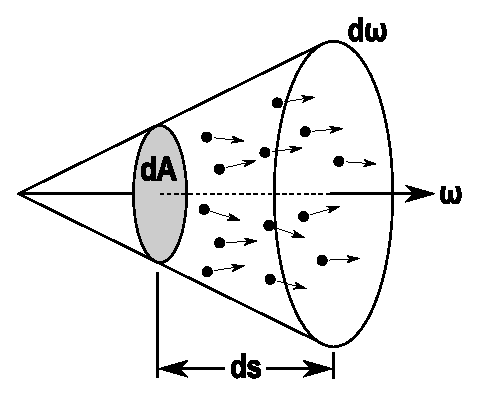
\includegraphics[height=0.3\textheight]{phasespacefluxsurface.eps}
		\caption{Teilchen, die das infinitesimale Flächenelement $dA$ durchqueren und sich in eine Richtung innerhalb des infinitesimalen Raumwinkelelements $d\omega$ um die Flächennormale $\omega$ von $dA$ bewegen.}
		\label{fig:phasespacefluxsurface}
	\end{figure}
	Der Phasenraumfluss ist wie die Phasenraumdichte eine fundamentale Größe, aus der wir alle anderen Observablen ableiten können. Im Folgenden werden wir uns meist auf den Phasenraumfluss beziehen.
		
	Unser Ziel ist es nun eine Bilanzgleichung für Teilchen in einem beliebigen Teil $V \times \Omega$ des Phasenraums (s. Abb.~(\ref{fig:phasespacevolume})) aufzustellen. Dafür sei $V \subset \mathbb{R}^3$ ein Teilvolumen des $\mathbb{R}^3$ und $\Omega \subset \mathcal{S}^2$ ein beliebiger Raumwinkel aus der Einheitskugel $\mathcal{S}^2$. Dazu untersuchen wir Ursachen für eine Veränderung der Teilchenzahl in unserem betrachteten Phasenraumvolumen $V \times \Omega$.
	\begin{figure}
		\centering
		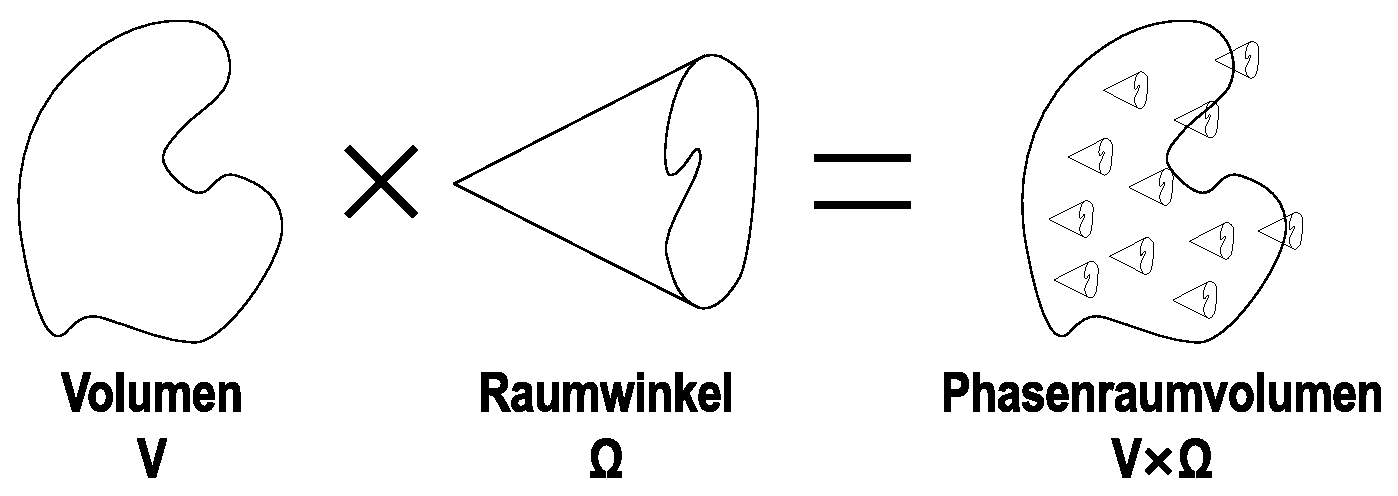
\includegraphics[width=0.8\textwidth]{phasespacevolume.eps}
		\caption{Darstellung einer Teilmenge $V \times \Omega$ des Phasenraums. Sie repräsentiert alle Teilchen, die sich innerhalb des Volumens $V$ befinden und sich in eine Richtung $\omega\in\Omega$ bewegen.}
		\label{fig:phasespacevolume}
	\end{figure}

	Zur {\em Emission} zählt jeder Prozess, der neue Teilchen erzeugt, wie z.B. chemische Reaktionen, thermische Emission oder Kernfusion. Emission innerhalb von $V$ in eine Richtung $\omega\in\Omega$ stellt also eine Quelle für Teilchen dar. Nach der Emission bewegen sich die Teilchen in unserem Modell gradlinig mit konstanter Geschwindigkeit bis eine Wechselwirkung mit dem Medium stattfindet. Bewegt sich ein Teilchen bei seiner gradlinigen Bewegung in das Volumen $V$ hinein oder aus ihm heraus und bewegt es sich dabei in eine Richtung innerhalb von $\Omega$, so ändert dies ebenfalls die Bilanz. In diesem Fall sprechen wir von {\em Durchströmen}. Findet eine {\em Kollision} des Teilchens mit dem Medium statt, kann das Teilchen entweder absorbiert oder gestreut werden. Wird es absorbiert wirkt dies als Teilchensenke. Wird es gestreut, dann kann es, je nach Richtung vor und nach der Kollision, entweder keinen Einfluss auf die Teilchenbilanz haben (Bewegungsrichtung vor und nach der Kollision entweder innerhalb oder außerhalb von $\Omega$), es kann herausgestreut werden (Bewegungsrichtung vor der Kollision innerhalb und nach der Kollision ausserhalb von $\Omega$) oder aber hineingestreut werden (Bewegungsrichtung vor der Kollision ausserhalb und nach der Kollision innerhalb von $\Omega$) werden.
	
	Um die einzelnen Beiträge dieser Prozesse zur Teilchenbilanz quantitativ zu erfassen führen wir die Teilchenzahl $$N(t):=\int_\Omega \int_V n(\location{r},\omega,t)\,d\location{r}\,d\omega$$ ein. Sie gibt an wieviele Teilchen sich zum Zeitpunkt $t$ im Phasenraumvolumen $V \times \Omega$ befinden. Durch die eben beschriebenen Prozesse ändert sich $N(t)$ normalerweise mit der Zeit. Ist die Zeit, die ein Teilchen benötigt um das System zu durchqueren, klein gegenüber der typischen Zeitskala für Veränderung des Systems, können wir annehmen, dass sich die Teilchenzahl überall im dynamischen Gleichgewicht befindet, d.h. dass Teilchen ständig aus dem Phasenraumvolumen hinein- und hinausströmen, erzeugt, absorbiert und gestreut werden, aber sich alle Prozesse die Waage halten, $N(t)$ also stationär ist:$$\frac{dN}{dt}=0\qquad\left[\frac{1}{\text{s}}\right].$$ Teilen wir diese Änderung von $N$ mit der Zeit auf die erläuterten Prozesse auf, sind wir bei der Bilanzgleichung angelangt:$$\frac{dN}{dt}=\begin{bmatrix}\text{Änderung}\\ \text{durch}\\ \text{Emission}\end{bmatrix}+\begin{bmatrix}\text{Änderung}\\ \text{durch}\\ \text{Durchströmung}\end{bmatrix}+\begin{bmatrix}\text{Änderung}\\ \text{durch}\\ \text{Kollisionen}\end{bmatrix}=0.$$ Wir leiten nun für jeden dieser Ausdrücke einen Formelausdruck her.
	Die Änderung aufgrund von Emission nennen wir $$\mathbf{E}=\int_\Omega \int_V q(\location{r},\omega)\,d\location{r}\,d\omega\qquad\left[\frac{1}{\text{s}}\right],$$ wobei wir die Quellfunktion $q$ (mit Einheit $\text{m}^{-3}\text{sr}^{-1}\text{s}^{-1}$) eingeführt haben, die für jeden Ort $\location{r}$ und jede Raumrichtung $\omega$ die Anzahl pro Sekunde, Einheitsvolumen und Einheitsraumwinkel erzeugter Teilchen angibt. Hinein- und herausströmende Teilchen erzeugen eine Teilchenrate
	$$\mathbf{S}=\int_\Omega \int_{\partial V} \phi(\location{r},\omega)(\omega \cdot \location{n}(\location{r}))d\location{r}\,d\omega,$$
	die wir durch Integrieren über $\partial V$ (die Oberfläche von V) erhalten. Hierbei steht $\location{n}(\location{r})$ für die Flächennormale am Ort $\location{r}\in\partial V$. Das Skalarprodukt zwischen Bewegungsrichtung $\omega$ und Flächennormalen sorgt für das richtige Vorzeichen, wobei ein positiver Wert Teilchenverlust bedeutet.
	Der letzte Beitrag $\mathbf{C}$ trägt den Kollisionen Rechnung. Da Teilchen nur mit dem Medium, nicht aber untereinander interagieren, muss die Kollisionsrate unabhängig von $\phi$ sein. Wir unterteilen $\mathbf{C}$ in einen Absorptionsteil und einen Streuanteil:
	$$\mathbf{C}=\mathbf{C}_\text{abs}+\mathbf{C}_\text{sca}.$$
	Wir nehmen an, dass die Wahrscheinlichkeit einer Absorption proportional zur zurückgelegten Distanz im Medium ist und unabhängig von der Bewegungsrichtung, was gleichbedeutend mit der Annahme eines isotropen Mediums ist. Die Proportionalitätskonstante am Ort $\location{r}$ nennen wir den (Volumen-)Absorptionsquerschnitt $\kappa(\location{r})$ ($[\kappa]=\frac{1}{\text{m}}=\frac{m^2}{m^3}$). Die zugehörige Teilchenrate ist
	$$\mathbf{C}_\text{abs}=\int_\Omega \int_V \kappa(\location{r})\phi(\location{r},\omega)\,d\location{r}\,d\omega.$$
	Die genauen Mechanismen der Streuung werden bei der Lösung der Wellengleichung behandelt (Mie--Theorie). In unserem Teilchentransport repräsentieren wir diese Streumodelle durch die Streuphasenfunktion $k(\location{r},\omega,\omega')$ und den Volumenstreuquerschnitt $\sigma(\location{r})$. Dabei gibt $k(\location{r},\omega,\omega')$ bei Streuung eines aus Richtung $\omega$ kommenden Teilchens am Ort $\location{r}$ die Wahrscheinlichkeit pro Einheitsraumwinkel an, nach $\omega'$ gestreut zu werden. Da ein gestreutes Teilchen erhalten bleibt, gilt für $k$ die Normierungsbedingung
	\begin{equation}\label{eq:k_norm_req}
	  \int_{\mathcal{S}^2} k(\location{r},\omega,\omega')\,d\omega'=1.
	\end{equation}
	Außerdem ist $k$ symmetrisch bezüglich Vertauschung der Bewegungsrichtungen vor und nach der Streuung:
	$$k(\location{r},\omega,\omega')=k(\location{r},\omega',\omega)\quad \forall\:\omega,\omega'\in\mathcal{S}^2.$$
	Beide Bedingungen werden z.B. durch die isotrope Streuphasenfunktion $$k_\text{iso}(\location{r},\omega,\omega')=\frac{1}{4\pi}$$ erfüllt.
	Wie bei der Absorption, nehmen wir an, dass die Wahrscheinlichkeit eines Teilchens gestreut zu werden von der durch das Medium zurückgelegten Distanz, nicht aber von der Bewegungsrichtung abhängt. Wir teilen $\mathbf{C}_\text{sca}$ weiter auf, in einen Teil
	$$\mathbf{C}_\text{out}=\int_\Omega \int_V \int_{\mathcal{S}^2} \sigma{(\location{r})}k(\location{r},\omega,\omega')\phi(\location{r},\omega)\,d\omega'\,d\location{r}\,d\omega,$$
	der herausgestreute Teilchen berücksichtigt, sowie einen Teil
	$$\mathbf{C}_\text{in}=\int_\Omega \int_V \int_{\mathcal{S}^2} \sigma{(\location{r})}k(\location{r},\omega',\omega)\phi(\location{r},\omega')\,d\omega'\,d\location{r}\,d\omega$$
	entsprechend für hineingestreute Teilchen. Dabei sollte erwähnt werden, dass sowohl $\mathbf{C}_\text{out}$ als auch $\mathbf{C}_\text{in}$ Teilchen berücksichtigen, deren Richtung vor und nach der Streuung in $\Omega$ liegt, was weder einem Zuwachs noch einem Verlust an Teilchen entspricht. Da für unsere Bilanz aber immer nur die Differenz von $\mathbf{C}_\text{out}$ und $\mathbf{C}_\text{in}$ betrachtet wird, hebt sich dieser Teil wieder heraus. Alternativ könnten wir auch über $\mathcal{S}^2 \setminus \Omega$ integrieren, was zu einer komplizierteren Rechnung, aber zu keinem anderen Endergebnis führen würde. Fügen wir die Einzelterme zusammen und ordnen nach Zuwächsen und Verlusten sieht unsere Bilanzgleichung für die Teilchenraten in $V \times \Omega$ wie folgt aus:
	$$\underbrace{\mathbf{S}+\mathbf{C}_\text{abs}+\mathbf{C}_\text{out}}_\text{Verluste}=\underbrace{\mathbf{E}+\mathbf{C}_\text{in}}_\text{Zuwächse}$$
	Es fällt bei der Betrachtung der Formeln für die einzelnen Terme auf, dass alle Terme bis auf $\mathbf{S}$ Volumenintegrale über $V$ enthalten. $\mathbf{S}$ enthält stattdessen ein Oberflächenintegral über $\partial V$. Mit dem Gauss'schen Satz erhalten wir
	$$\mathbf{S}=\int_\Omega \int_V \omega \cdot (\nabla\phi)(\location{r},\omega)\,d\location{r}\,d\omega,$$
	wobei wir $$\nabla \cdot(\omega\phi)=\omega\cdot(\nabla\phi)+\underbrace{(\nabla\omega)}_{=0}\cdot\,\phi$$ benutzt haben.
	
	In der Bilanzgleichung treten jetzt nur noch Volumenintegrale über $V \times \Omega$ auf. Da $V$ und $\Omega$ beliebig gewählt waren, erhalten wir den lokalen Zusammenhang:
	\begin{multline*}
	  \omega\cdot\nabla\phi(\location{r},\omega)+\kappa(\location{r})\phi(\location{r},\omega)+\int_{\mathcal{S}^2}\sigma(\location{r})k(\location{r},\omega,\omega')\phi(\location{r},\omega)d\omega' \\
	  =q(\location{r},\omega)+\int_{\mathcal{S}^2}\sigma(\location{r})k(\location{r},\omega',\omega)\phi(\location{r},\omega')d\omega'.
	\end{multline*}
	Da beim $\mathbf{C}_\text{out}$--Integral $\sigma$ und $\phi$ nicht von der Integrationsvariable abhängen und sich das verbleibende Integral aufgrund der Normierung (\ref{eq:k_norm_req}) vereinfacht, ergibt sich schließlich die Bilanzgleichung in Gestalt einer Integro--Differentialgleichung in $\phi$:
	\begin{equation}\label{eq:particle_balance_equation}
	  \omega\cdot\nabla\phi(\location{r},\omega)+\left(\kappa(\location{r})+\sigma(\location{r})\right)\phi(\location{r},\omega)
	  =q(\location{r},\omega)+\sigma(\location{r})\int_{\mathcal{S}^2}k(\location{r},\omega',\omega)\phi(\location{r},\omega')d\omega'
	\end{equation}
	Im folgenden Abschnitt stellen wir den Bezug zwischen unseren abstrakten Teilchentransportgrößen und physikalischen Strahlungsgrößen her.

	\section{Phänomenologische Strahlungsgrößen}\label{subsec:strahlungsgroessen}
	Im vorigen Abschnitt haben wir das Strahlungstransportproblem bewusst auf ein Teilchentransportproblem (mit abstrakten Teilchen statt Photonen) reduziert um einerseits eine klare Herleitung zu ermöglichen und um andererseits die Verwandtschaft zu anderen Transportproblemen (wie z.B. Neutronentransport) offensichtlich zu machen. Für den Anschluss zu radiometrischen Strahlungsgrößen, ersetzen wir die abstrakten Teilchen durch Photonen. Photonen haben zwei Eigenschaften die wir berücksichtigen müssen. Sie bewegen sich konstant mit Lichtgeschwindigkeit, d.h. wir können die vorher gebrauchte allgemeine Teilchengeschwindigkeit $v$ gleich $\text{c}$ setzen. Außerdem besitzt jedes Photon eine Energie, die mit seiner Frequenz $\nu$ über 
	$$E=h\nu \qquad[J]$$
	zusammenhängt. Dabei bezeichnet $h$ das Planck'sche Wirkungsquantum.
	Jeder Frequenz $\nu$ können wir ein monochromatisches Transportproblem zuordnen, dessen Lösung in Form eines Phasenraumflusses $\phi_\nu$ die Photonenfrequenz als Index trägt.
	Die {\em spezifische Intensität} $I_\nu(\location{r},\omega)$ erhalten wir nun aus dem Phasenraumfluss bzw. der Phasenraumdichte gemäß
	\begin{align}\label{eq:intensity_def}
		I_\nu(\location{r},\omega)d\nu & = h\nu\,\phi_\nu(\location{r},\omega)\\
		                       & = c h\nu\,n_\nu(\location{r},\omega) \qquad \left[\frac{\text{W}}{\text{m}^2\text{sr}}\right] \nonumber
	\end{align}
	Sie gibt an, wieviel Joule am Ort $\location{r}$ pro Sekunde durch eine Einheitsfläche mit Flächennormale $\omega$ pro Einheitsraumwinkel in Richtung $\omega$ und pro Frequenzintervall durch Photonen mit Frequenz $\nu$ transportiert wird:
	$$dE_\nu=I_\nu(\location{r},\omega) dA\,dt\,d\omega\,d\nu.$$
	Wir führen außerdem die {\em spezifische Emissivität} $\varepsilon_\nu$ ein. Wir erhalten Sie aus der Quellfunktion $q_\nu$ durch
	\begin{equation}\label{eq:emissivity_def}
		\varepsilon_\nu(\location{r},\omega)d\nu = h\nu\,q_\nu(\location{r},\omega) \qquad \left[\frac{\text{W}}{\text{m}^3\text{sr}}\right].
	\end{equation}
	
	Multiplizieren wir die abstrakte Transportgleichung (\ref{eq:particle_balance_equation}) mit $h\nu$ und benutzen wir die Beziehungen (\ref{eq:intensity_def}, \ref{eq:emissivity_def}) erhalten wir mit
	\begin{equation}\label{eq:stg_diff}
	  \omega\cdot\nabla I_\nu(\location{r},\omega)+\left(\kappa_\nu(\location{r})+\sigma_\nu(\location{r})\right)I_\nu(\location{r},\omega)
	  =\varepsilon_\nu(\location{r},\omega)+\sigma_\nu(\location{r})\int_{\mathcal{S}^2}k_\nu(\location{r},\omega',\omega)I_\nu(\location{r},\omega')d\omega'
	\end{equation}
	die {\em Strahlungstransportgleichung in differentieller Form}. Sie stellt eine Integro--Differentialgleichung für $I_\nu$ auf dem 5--dimensionalen Phasenraum $\mathbb{R}^3 \times \mathcal{S}^2$ dar und kann für jede Frequenz $\nu$ getrennt gelöst werden. Sie gibt für jede Kombination aus Ort $\location{r}$ und Ausbreitungsrichtung $\omega$ das lokal zu erfüllende Gleichgewicht aus Verlusten (linke Seite) und Zuwächsen (rechte Seite) an.
	
	Wir fassen die Verluste durch Absorption und Streuung mit dem {\em Vo\-lu\-men\-ex\-tink\-ti\-ons\-quer\-schnitt}
	$$\xi_\nu(\location{r}):=\kappa_\nu(\location{r})+\sigma_\nu(\location{r}) \qquad\left[\frac{1}{m}\right]$$
	zusammen, wodurch wir (\ref{eq:stg_diff}) auch kürzer als
	\begin{equation}\label{eq:stg_diff2}
	  \omega\cdot\nabla I_\nu(\location{r},\omega)+\xi_\nu(\location{r})I_\nu(\location{r},\omega)
	  =\varepsilon_\nu(\location{r},\omega)+\sigma_\nu(\location{r})\int_{\mathcal{S}^2}k_\nu(\location{r},\omega',\omega)I_\nu(\location{r},\omega')d\omega'
	\end{equation}
	schreiben können.
	Außerdem definieren wir die dimensionslose {\em optische Tiefe}
	\begin{equation*}
		\tau_\nu(\location{r}_1,\location{r}_2):=\int_{s=0}^{\|\location{r}_2-\location{r}_1\|} \xi_\nu(\location{r}_1+s(\location{r}_2 - \location{r}_1))\,ds,
	\end{equation*}
	als Maß für die Undurchsichtigkeit des Mediums bei der Frequenz $\nu$ zwischen zwei Orten $\location{r}_1$ und $\location{r}_2$. Vereinfachen wir Gleichung (\ref{eq:stg_diff2}), indem wir Quellen zu Null setzen und eine beliebige Richtung $\omega$ wählen, so gelangen wir zur gewöhnlichen Differentialgleichung
	$$I_\nu'(s)+\xi_\nu(s)I_\nu(s)=0,$$
	die durch
	\begin{equation}
		I_\nu(s)=I_\nu(0)\:\text{exp}\left(-\int_{s'=0}^s \xi_\nu(s')\right)=I_\nu(0)\:\text{exp}\left(-\tau_\nu(0,s)\right)
		\label{eq:exponentialdecay}
	\end{equation}
	gelöst wird. Die optische Tiefe beschreibt also eine exponentielle Abschwächung einfallender Intensität. Nach der Definition der verschiedenen phänomenologischen Strahlungsgrößen schauen wir uns nun an, wie ihre Messung aufgefasst und mathematisch definiert werden kann.
	
	
	\section{Die Messgleichung}\label{sec:measurement_equation}
	Mit dem Strahlungsintensitätsfeld, das aus der Gesamtheit aller spezifischen Intensitäten $I_\nu$ besteht, meinen wir die Funktion
	$$I:\mathbb{R}_+\times\mathbb{R}^3\times\mathcal{S}^2\to\mathbb{R}_+\;,\qquad (\nu,\location{r},\omega)\mapsto I_\nu(\location{r},\omega),$$
	die vom 6--dimensionalen Raum aller Frequenzen, Orte und Raumrichtungen auf die lokale spezifische Intensität abbildet.
	
	Funktionen dieser Art bilden einen Skalarproduktraum. Das Null--Element ist die konstant auf Null abbildende Funktion. Zwei Funktionen lassen sich punktweise addieren und ergeben so eine neue Funktion, die auch nach $\mathbb{R}_{\geq 0}$ abbildet. Das Skalarprodukt zwischen zwei Funktionen $f$ und $g$ ist schließlich mit
	$$\langle f,g\rangle=\int_{\mathbb{R}_+} \int_{\mathbb{R}^3} \int_{\mathcal{S}^2} f(\nu,\location{r},\omega)g(\nu,\location{r},\omega)\,d\omega\,d\location{r}\,d\nu$$
	gegeben.
	
	Mit diesem funktionalanalytischen Handwerkszeug definieren wir eine Messung als das Skalarprodukt zwischen unserem Strahlungsintensitätsfeld $I$ und einer {\em Sensitivitätsfunktion} $W$, welche die Stärke der Gewichtung angibt, mit der die spezifische Intensität der Frequenz $\nu$ am Ort $\location{r}$ in Richtung $\omega$ in den Messwert eingeht. Die entsprechende Formel
	\begin{equation}\label{eq:messgleichung}
		M^{(i)}:=\langle W^{(i)},I\rangle=\int_{\mathbb{R}_+} \int_{\mathbb{R}^3} \int_{\mathcal{S}^2} W^{(i)}(\nu,\location{r},\omega)I_\nu(\location{r},\omega)\,d\omega\,d\location{r}\,d\nu
	\end{equation}
	nennen wir {\em Messgleichung} (für den $i$--ten Sensor). Für monochromatische Messungen führen wir zusätzlich noch 
	\begin{equation}\label{eq:messgleichung_mono}
		M_\nu^{(i)}:=\langle W_\nu^{(i)},I_\nu\rangle=\int_{\mathbb{R}^3} \int_{\mathcal{S}^2} W_\nu^{(i)}(\location{r},\omega)I_\nu(\location{r},\omega)\,d\omega\,d\location{r}
	\end{equation}
	ein, womit wir (\ref{eq:messgleichung}) auch als
	\begin{equation}\label{eq:messgleichung_frommonos}
		M^{(i)}=\int_{\mathbb{R}_+} M_\nu^{(i)}\,d\nu
	\end{equation}
	schreiben können.
	Diese Abstraktion erlaubt uns größtmögliche Freiheit beim kreieren virtueller Sensoren. Beispielsweise könnte $W$ nur in einem kleinen Volumen und einem kleinen Raumwinkel, aber bei allen Frequenzen, nichtverschwindend sein, und so einen Sensor zur Messung der Gesamt--Intensität an einem bestimmten Ort in eine bestimmte Richtung repräsentieren. Ebenso kann durch gleichstarke Gewichtung aller Raumrichtungen die mittlere Intensität gemessen werden.
	
	Was zunächst nur als theoretisches Konstrukt ohne praktischen Nutzen erscheint, wird sich später in Verbindung mit Monte--Carlo--Sampling als vielseitiges und effizientes Werkzeug erweisen.
	
	
	\section{Übersicht etablierter Lösungsverfahren}
	TODO: Übersicht benutzter Lösungsverfahren, Meilensteine (wann zum ersten mal Polarisation gerechnet?, Warum etablieren sich MC-Verfahren so spät?, etc...)
		
	\chapter{Pfadintegralformulierung der Strahlungstransportgleichung}\label{chapter:path_radiative_transfer}
	In diesem Abschnitt leiten wir eine alternative mathematische Formulierung der Strahlungstransportgleichung einerseits und ihrer Lösung (genau genommen, Messungen der Lösung im Sinne von (\ref{eq:messgleichung})) andererseits her. Dies führt uns durch die verschiedenen auf das Problem eingenommenen Blickwinkel zu einem besseren Verständnis von Strahlungstransport und gibt uns darüber hinaus einen neuen Ansatzpunkt zur effizienten Lösung des Strahlungstransportproblems.
	
	Die Idee zu dieser Formulierung kommt aus der Dissertation von \citet{Veach:1997p9136}, wird aber schon in \citep{Arvo:1995p9257} vorgestellt. Beide Dissertationen behandeln allerdings nur den Strahlungstransport zwischen Oberflächen. In der Arbeit von \citet{Pauly:2000p5705} wird dies auf partizipierende Medien ausgedehnt. Aus \citep{Arvo:1993p9035} stammt außerdem die Herleitung der integralen Form der Strahlungstransportgleichung.
	
	
	\section{Strahlungstransportgleichung in integraler Form}
	In differentieller Form nimmt die Strahlungstransportgleichung, wie wir in Abschnitt (\ref{subsec:strahlungsgroessen}) gesehen haben, folgende Gestalt an:
		\begin{equation}
			\omega \cdot \nabla I(\location{r},\omega)+\overbrace{\left(\kappa(\location{r})+\sigma(\location{r})\right)}^{=:\xi(\location{r})}I(\location{r},\omega)=\varepsilon(\location{r},\omega)+\sigma(\location{r}) \int_{\mathcal{S}^2} k(\location{r},\omega',\omega)I(\location{r},\omega') d\omega'.
			\label{eq:diff.STG}
		\end{equation}
	Für diesen und die folgenden Abschnitte lassen wir dabei den Index $\nu$ aus übersichtsgründen weg, womit gemeint ist, dass wir stellvertretend für alle Frequenzen ein einzelnes monochromatisches Strahlungstransportproblem einer beliebigen Frequenz nehmen. Wenn wir zum polychromatischen Fall zurückkehren führen wir die Indizes wieder ein.
	
	Schreiben wir das Skalarprodukt zwischen $\omega$ und dem $\nabla$--Operator als Richtungsableitung
	\newcommand{\dds}{\frac{\text{d}}{\text{d}s}}
	\newcommand{\ddszero}{\left. \dds \right|_{s=0}}
	\begin{equation*}
		\omega \cdot \nabla I(\location{r},\omega)
		=  \ddszero I(\location{r}+s\,\omega,\omega)
		=  -\ddszero I(\location{r}-s\,\omega,\omega)
	\end{equation*}
	können wir (\ref{eq:diff.STG}) als
	\begin{multline}
		\dds I(\location{r}-s\,\omega,\omega) - \xi(\location{r}-s\,\omega)I(\location{r}-s\,\omega,\omega) = \\-\varepsilon(\location{r}-s\,\omega,\omega) -\sigma(\location{r}-s\,\omega) \int_{\mathcal{S}^2} k(\location{r}-s\,\omega,\omega',\omega)I(\location{r}-s\,\omega,\omega') \text{d}\omega'
		\label{eq:diff.STGtranslated}
	\end{multline}
	umschreiben. Dabei haben wir die Beschränkung $s=0$ fallengelassen, was die Korrektheit der Umformung aber nicht ändert. Mit den Abkürzungen
	\begin{align*}
		{\hat I}(s)&:=I(\location{r}-s\,\omega,\omega) \\
		Q(\location{r},\omega)&:= \varepsilon(\location{r},\omega)+\sigma(\location{r}) \int_{\mathcal{S}^2} k(\location{r},\omega',\omega)I(\location{r},\omega') d\omega' \\
		{\hat Q}(s)&:=Q(\location{r}-s\,\omega,\omega)\\
		{\hat \xi}(s)&:=\xi(\location{r}-s\,\omega) \\
		{\hat \tau}(s)&:= \int_{s'=0}^{s} {\hat \xi}(s') \text{d}s'
	\end{align*}
	wird aus (\ref{eq:diff.STGtranslated})
	\begin{equation}
		\dds {\hat I}(s) - {\hat \xi}(s){\hat I}(s)= -{\hat Q}(s) \qquad |\cdot e^{-{\hat \tau}(s)}.
		\label{eq:diff.STGhatted}
	\end{equation}
	Gleichung (\ref{eq:diff.STGhatted}) ist eine gewöhnliche Differentialgleichung die sich mit
	\begin{align}
		(\ref{eq:diff.STGhatted})\Leftrightarrow\qquad \dds \left(e^{-{\hat \tau}(s)} {\hat I}(s)\right)&= -e^{-{\hat \tau}(s)} {\hat Q}(s) \qquad | \int_{s'=0}^s (\cdot)\text{d}s' \nonumber \\
		\Leftrightarrow\qquad e^{-{\hat \tau}(s)} {\hat I}(s) - {\hat I}(0) &= -\int_{s'=0}^s e^{-{\hat \tau}(s')} {\hat Q}(s') \text{d}s' \nonumber \\
		\Leftrightarrow\qquad {\hat I}(0) &= e^{-{\hat \tau}(s)} {\hat I}(s) + \int_{s'=0}^s e^{-{\hat \tau}(s')} {\hat Q}(s') \text{d}s' \label{eq:diff.STGpreintegral}
	\end{align}
	leicht nach ${\hat I}(0)$ auflösen lässt. Obwohl ${\hat Q}(s)$ lokal die Intensität $I$ über alle Raumrichtungen integriert, dürfen wir für die Lösung von (\ref{eq:diff.STGhatted}) $Q$ als unabhängig von $I$ behandeln, da die Schnittmenge zwischen der Geraden im Raum, auf der wir die Differentialgleichung lösen, und der Menge aller Raumrichtungen $\mathcal{S}^2$ bei der Integration über alle Raumrichtungen eine Nullmenge ist und somit für physikalisch relevante Strahlungsintensitätsfelder (d.h. solche, die hinreichend stetig/beschränkt bzw. keine Delta--Distribution sind) keinen Beitrag zum Integral leistet.
	Setzen wir in (\ref{eq:diff.STGpreintegral}) für die Abkürzungen wieder die ursprünglichen Ausdrücke ein, erhalten wir die {\em Strahlungstransportgleichung in integraler Form}:
	\begin{multline}
		I(\location{r},\omega) = e^{-\tau(\location{r},\location{r}-s\,\omega)} {\hat I}(\location{r},\location{r}-s\,\omega) + \int_{s'=0}^\infty e^{-\tau(\location{r},\location{r}-s\,\omega)} \;\cdot \\
		\quad\cdot\left( \varepsilon(\location{r}-s'\,\omega,\omega) + \sigma(\location{r}-s'\,\omega)
		\left[ \int_{\mathcal{S}^2} k(\location{r}-s'\,\omega,\omega',\omega)I(\location{r}-s'\,\omega,\omega') \text{d}\omega'\right] \right) \text{d}s'
		\label{eq:int.STG}
	\end{multline}
	Nehmen wir nun als Randbedingungen an, dass in unendlich großer Entfernung keine Lichtquellen existieren, d.h. $\forall \omega \in \mathcal{S}^2 : I(\location{r}=-\infty\cdot\omega,\omega)=0$, dann vereinfacht sich (\ref{eq:int.STG}) zu
	\begin{multline}
		I(\location{r},\omega) = \int_{s'=0}^\infty e^{-\tau(\location{r},\location{r}-s\,\omega)} \;\cdot \\
		\quad\cdot\left( \varepsilon(\location{r}-s'\,\omega,\omega) + \sigma(\location{r}-s'\,\omega)
		\left[ \int_{\mathcal{S}^2} k(\location{r}-s'\,\omega,\omega',\omega)I(\location{r}-s'\,\omega,\omega') \text{d}\omega'\right] \right) \text{d}s'
		\label{eq:int.STGdarkbg}
	\end{multline}


	\section{Strahlungstransportgleichung in Operator--Form}
	Schauen wir uns die einzelnen Teile der Gleichung (\ref{eq:int.STGdarkbg}) genauer an.
	Der innere Teil von (\ref{eq:int.STGdarkbg}) in eckigen Klammern summiert an einem festen Ort ($\location{r}-s'\,\omega$), mit der Streuphasenfunktion $k$ gewichtet, die einfallenden Intensitäten auf, die in Richtung $\omega$ gestreut werden. Anschließend skaliert der Volumenstreuquerschnitt die aufintegrierte Intensität entsprechend dem lokal vorhandenen Medium und gibt dabei dem Ausdruck die Einheit einer Emissivität.
	Der restliche äußere Teil der Gleichung addiert die eben gewonnene Emissivität durch Einstreuung zu der lokal durch Ausstrahlung erzeugten Emissivität an jedem Punkt auf einer Geraden hinter dem Punkt $\location{r}$ und summiert die mit einem der optischen Tiefe entsprechenden Abschwächungsfaktor gewichteten, in Richtung $\omega$ zeigenden, Emissivitäten, entlang der Geraden zur Gesamtintensität am Ort $\location{r}$ in Richtung $\omega$ auf.
	Der Gesamtausdruck lässt sich durch Einführung zweier neuer Operatoren
	\begin{align*}
		\left(\mathbf{G}\varepsilon\right)(\location{r},\omega)&:=\int_{s'=0}^\infty e^{-\tau(\location{r}-s' \omega,\location{r})}\varepsilon(\location{r}-s' \omega,\omega) ds' \\
		\left(\mathbf{K}I\right)(\location{r},\omega)&:=\sigma(\location{r})\int_{S^2} k(\location{r},\omega',\omega) I(\location{r},\omega') d\omega'
	\end{align*}
	\begin{equation*}
		\mathbf{G} : \varepsilon(\location{r},\omega) \mapsto I(\location{r},\omega) , \qquad
		\mathbf{K} : I(\location{r},\omega) \mapsto \varepsilon(\location{r},\omega)
	\end{equation*}
	in elementarere Prozesse aufteilen. Wir nennen $\mathbf{G}$ den sogenannten {\em Fortpflanzungs--Operator} und $\mathbf{K}$ den {\em Streu--Operator}. Beides sind Integraloperatoren auf dem Raum der Funktionen $f : \mathbb{R}^3 \times \mathcal{S}^2 \to \mathbb{R}_+$, die vom Teilchen--Phasenraum auf die positiven reellen Zahlen abbilden. Beide haben komplementäre Lokalitäten. Während $\mathbf{K}$ lokal im Ort über alle Raumrichtungen integriert, ist $\mathbf{G}$ lokal in der Raumrichtung und integriert über alle Orte entlang einer Geraden im Raum. Dabei bildet $\mathbf{K}$ von einem Strahlungsintensitätsfeld auf ein Emissivitätsfeld ab. Bei $\mathbf{G}$ ist es umgekehrt, es macht aus einem Emissivitätsfeld wieder ein Strahlungsintensitätsfeld.
	Mit diesen neuen Operatoren wird aus Gleichung (\ref{eq:int.STGdarkbg}) die {\em Operatorform der Strahlungstransportgleichung}
	\begin{equation}
		I=\mathbf{G}(\varepsilon + \mathbf{K}I),
		\label{eq:op.STG}
	\end{equation}
	die wir nach $I$ auflösen können:
	\begin{align}
		(\ref{eq:op.STG}) \Leftrightarrow I&=\mathbf{G}\varepsilon + \mathbf{GK}I \nonumber \\
		\Leftrightarrow (\mathbf{1}-\mathbf{GK})I &= \mathbf{G}\varepsilon \nonumber \\
		\Leftrightarrow I &= (\mathbf{1}-\mathbf{GK})^{-1}\mathbf{G}\varepsilon \label{eq:op.STGinvert} \\
		\Leftrightarrow I &= \sum_{k=0}^\infty (\mathbf{GK})^k \mathbf{G}\varepsilon \label{eq:op.STGneumann} \\
		&=\mathbf{G}\varepsilon + \mathbf{GKG}\varepsilon + \mathbf{GKGKG}\varepsilon + \hdots \label{eq:op.STGneumann.explicit} \\
		\Leftrightarrow I &=\sum_{k=0}^\infty \mathbf{G} (\mathbf{KG})^k \varepsilon \label{eq:op.STGkg}
	\end{align}
	Damit ist das Strahlungstransportproblem formal gelöst! Dabei haben wir den auftretenden invertierten Operator (\ref{eq:op.STGinvert}) durch eine Neumann--Reihe (\ref{eq:op.STGneumann}) ersetzt. Dies ist dann zulässig wenn die Operatornorm des Operators $\mathbf{GK}$ kleiner als eins ist und damit sichergestellt ist, dass die Neumann--Reihe konvergiert. Für alle praktisch relevanten Probleme ist dies der Fall \citep[s.][Theorem 12 und 13]{Arvo:1995p9257}. Physikalisch lässt sich das Gleichgewichts--Strahlungsintensitätsfeld als Summe aus Intensitätsfeldern verstehen, die durch Photonen mit unterschiedlich vielen Streuereignissen auf ihrem Weg von der Emission aus einer Lichtquelle bis zu ihrer Messung mit einem Messinstrument entstanden sind (wie in Schritt (\ref{eq:op.STGneumann.explicit}) deutlich wird). Dabei müssen Pfade jeder möglichen Länge (sprich Anzahl an Streuereignissen) berücksichtigt werden. Zwischen Emission und Messung wechseln sich dabei Fortpflanzung $\mathbf{G}$ und Streuung $\mathbf{K}$ ab. Im letzen Schritt (\ref{eq:op.STGkg}) haben wir $\mathbf{G}$ nach links ausgeklammert um den $\mathbf{KG}$--Operator herauszustellen.
	
	
	\section{KG--Operator in Volumenform}
	Schauen wir uns den $\mathbf{KG}$--Operator genauer an. Nachdem $\mathbf{KG}$ ein Emissivitätsfeld durch Fortpflanzung zu einem Intensitätsfeld aufintegriert hat, wird dieses durch die anschliessende Streuung erneut auf ein Emissivitätsfeld abgebildet:
	\begin{equation*}
		\mathbf{KG} : \varepsilon(\location{r},\omega) \mapsto \varepsilon(\location{r},\omega)
	\end{equation*}

	Setzen wir die Definitionen der Operatoren ein und fassen die Integrale zusammen:
	\begin{align*}
		\left(\mathbf{KG}\varepsilon\right)(\location{r},\omega)&=\sigma(\location{r}) \int_{\mathcal{S}^2} k(\location{r},\omega',\omega)\left[\int_{s'=0}^\infty e^{-\tau(\location{r}-s' \omega',\location{r})}\varepsilon(\location{r}-s' \omega',\omega') \text{d}s'\right] \text{d}\omega' \\
		&=\sigma(\location{r}) \int_{\mathcal{S}^2} \int_{s'=0}^\infty k(\location{r},\omega',\omega) e^{-\tau(\location{r}-s' \omega',\location{r})}\varepsilon(\location{r}-s' \omega',\omega') \underbrace{\text{d}s' \text{d}\omega'}_{=\frac{\text{d}\location{r}'}{s'^2}} \\
		&=\sigma(\location{r}) \int_{\mathbb{R}^3} k(\location{r},\omega',\omega) \frac{e^{-\tau(\location{r}',\location{r})}}{\|\location{r}-\location{r}'\|^2}\varepsilon(\location{r}',\omega') \,\text{d}\location{r}'
	\end{align*}
	Da wir durch Kombination der Integration über alle Raumrichtungen $\omega'$ und alle Entfernungen $s'$ den gesamten Raum abdecken, können wir die beiden Integrale zugunsten eines Volumenintegrals über den gesamten Raum und einen geometrischen Verdünnungsfaktor tauschen. Mit dem Ziel, später alle Integrationen zu Volumenintegralen zusammenzufassen, schreiben wir den $\mathbf{KG}$--Operator so um, dass alle expliziten Angaben von Entfernungen und Raumrichtungen durch eine raumpunktorientierte Notation ersetzt werden:
	\begin{multline}
		\left(\mathbf{KG}\varepsilon\right)(\location{r}_i \rightarrow\location{r}_{i+1})=\\
		\sigma(\location{r}_i) \int_{\mathbb{R}^3} k(\location{r}_{i-1}\rightarrow\location{r}_i\rightarrow\location{r}_{i+1})\frac{e^{-\tau(\location{r}_{i-1},\location{r}_i)}}{\|\location{r}_i-\location{r}_{i-1}\|^2}\varepsilon(\location{r}_{i-1} \rightarrow\location{r}_i)d\location{r}_{i-1}
		\label{eq:KGvolume_intermediate}
	\end{multline}
	Wir führen zusätzlich noch die Abkürzung
	\begin{align*}
		\scatter{i}\;&:=\sigma(\location{r}_i)k(\location{r}_{i-1}\rightarrow\location{r}_i\rightarrow\location{r}_{i+1})\\
			&=\sigma(\location{r}_i)k(\location{r}_i,\normalized{\location{r}_i-\location{r}_{i-1}},\normalized{\location{r}_{i+1}-\location{r}_i})
	\end{align*}
	ein, so dass wir (\ref{eq:KGvolume_intermediate}) zusammen mit den in Abschnitt \ref{subsec:nomenklatur} eingeführten Schreibweisen noch kompakter als
	\begin{equation}
		\left(\mathbf{KG}\varepsilon\right)_{(i,i+1)}=\int_{\mathbb{R}^3} \scatter{i}\frac{e^{-\tau_{(i-1,i)}}}{d_{(i-1,i)}^2}\varepsilon_{(i-1,i)}d\location{r}_{i-1}.
		\label{eq:KGvolume}
	\end{equation}
	schreiben können.


	\section{Pfadintegrallösung der Strahlungstransportgleichung}
	Wir setzen die Neumann--Reihen--Lösung (\ref{eq:op.STGkg}) in die monochromatische Meßgleichung (\ref{eq:messgleichung_mono}) ein und erhalten
	\begin{align}
		M_\nu&=\int_{\mathbb{R}^3}\int_{\mathcal{S}^2}W_\nu(\location{r},\omega) \left(\sum_{k=0}^\infty \mathbf{G} (\mathbf{KG})^k \varepsilon_\nu\right)(\location{r},\omega) \,\text{d}\omega \,\text{d}\location{r} \nonumber \\
		&=\sum_{k=0}^\infty \int_{\mathbb{R}^3}\int_{\mathcal{S}^2}W_\nu(\location{r},\omega) \left(\mathbf{G} (\mathbf{KG})^k \varepsilon_\nu\right)(\location{r},\omega) \,\text{d}\omega \,\text{d}\location{r} \nonumber \\
		&=\sum_{k=0}^\infty \int_{\mathbb{R}^3}\int_{\mathcal{S}^2}W_\nu(\location{r},\omega) \int_{s'=0}^\infty e^{-\tau_\nu(\location{r}-s' \omega,\location{r})} \left((\mathbf{KG})^k \varepsilon_\nu\right)(\location{r},\omega) \underbrace{\text{d}s' \,\text{d}\omega}_{=\frac{\text{d}\location{r}'}{s'^2}} \,\text{d}\location{r} \nonumber \\
		&=\sum_{k=0}^\infty \int_{\mathbb{R}^3}\int_{\mathbb{R}^3}W_\nu(\location{r}'\rightarrow\location{r}) \frac{e^{-\tau_\nu(\location{r}',\location{r})}}{\|\location{r}'-\location{r}\|^2} \left((\mathbf{KG})^k \varepsilon_\nu\right)(\location{r}'\rightarrow\location{r}) \,\text{d}\location{r}' \,\text{d}\location{r}.
		\label{eq:STGprepathsolution}
	\end{align}
	Durch rekursives Einsetzen von (\ref{eq:KGvolume}) in (\ref{eq:STGprepathsolution}) und Neuanordnung der Terme erhalten wir dann als Ergebnis einer monochromatischen Messung:
	\begin{equation}
		M_\nu=\sum_{k=0}^\infty \underbrace{\idotsint}_{(k+2)\text{--mal}}\varepsilon_{\nu,(0,1)}\left[\prod_{i=1}^k\frac{e^{-\tau_{\nu,(i-1,i)}}}{d_{(i-1,i)}^2}\scatter{i}\right]\frac{e^{-\tau_{\nu,(k,k+1)}}}{d_{(k,k+1)}^2} W_{\nu,(k,k+1)} \;\text{d}\location{r}_0 \dotsm \text{d}\location{r}_{k+1} .
		\label{eq:STGpathsolution}
	\end{equation}
	Das Ergebnis ist eine Summe aus reinen $(k+2)$--fachen Volumenintegralen über den ganzen Raum, wobei über den möglichen Start- und Endpunkt sowie die $k$ Streupunkte innerhalb des Photonenpfades integriert wird.
	Anschaulich müssen wir also die Beiträge von Pfaden jeder Anzahl an Streupunkten und jeder möglichen Anordnung von Emissions-, Streu- und Mess\-orten aufsummieren. Dies wird vielleicht klarer, wenn wir die ersten Terme der Summe explizit ausformulieren:
	\begin{align*}
		M_\nu&=\iint_{(\mathbb{R}^3)^2}\varepsilon_{\nu,(0,1)}\frac{e^{-\tau_{\nu,(0,1)}}}{d_{(0,1)}^2} W_{\nu,(0,1)} \;\text{d}\location{r}_0\text{d}\location{r}_1 \\
		&+\iiint_{(\mathbb{R}^3)^3}\varepsilon_{\nu,(0,1)}\frac{e^{-\tau_{\nu,(0,1)}}}{d_{(0,1)}^2}\scatter{1}\frac{e^{-\tau_{\nu,(1,2)}}}{d_{(1,2)}^2} W_{\nu,(1,2)} \;\text{d}\location{r}_0\text{d}\location{r}_1\text{d}\location{r}_2 \\
		&+\iiiint_{(\mathbb{R}^3)^4}\varepsilon_{\nu,(0,1)}\frac{e^{-\tau_{\nu,(0,1)}}}{d_{(0,1)}^2}\scatter{1}\frac{e^{-\tau_{\nu,(1,2)}}}{d_{(1,2)}^2}\scatter{2}\frac{e^{-\tau_{\nu,(2,3)}}}{d_{(2,3)}^2} W_{\nu,(2,3)} \;\text{d}\location{r}_0\text{d}\location{r}_1\text{d}\location{r}_2\text{d}\location{r}_3 \\
		&+\hdots
	\end{align*}
	Diese Form der Lösung des Strahlungstransportproblems hat mehrere Vorteile:
	\begin{itemize}
		\item{Die Lösung besitzt eine anschauliche Interpretation}
		\item{Die Lösung ist explizit, es muss keine implizite Integro--Differentialgleichung wie (\ref{eq:stg_diff}) gelöst werden}
		\item{Die Lösung ist ein reines Integrationsproblem und somit ein gutes Gegenstück zu hochdimensionalen Monte--Carlo--Integrations--Verfahren, wie wir in Abschnitt \ref{subsec:integrationsproblem_comparison} sehen werden}
	\end{itemize}
	Das polychromatische Messergebnis ergibt sich nun einfach durch Einsetzen von (\ref{eq:STGpathsolution}) in (\ref{eq:messgleichung_frommonos}).


	\section{Elimination der Neumann--Reihe}\label{sec:neumann_elimination}
	Unsere Darstellung der Lösung (\ref{eq:STGpathsolution}) des Strahlungstransportproblems besteht bisher aus einer unendlichen Summe von Integralen, was eine direkte Folge der Aufspaltung des Lösungsoperators aus (\ref{eq:op.STGinvert}) in seine Neumann--Reihe (\ref{eq:op.STGneumann}) ist. In dieser Form sind die Pfade in Klassen gleicher Länge (d.h. Anzahl an Streupunkten) eingeteilt, was die mathematische Behandlung vereinfacht, da die Fälle verschiedener Länge getrennt voneinander behandelt werden können. Gleichzeitig verleitet diese Darstellung jedoch dazu zu glauben, es wäre sinnvoll oder läge in der Natur der Sache, die Pfade unterschiedlicher Länge getrennt voneinander zu behandeln. Tatsächlich gibt es aber keinen physikalischen Grund dafür, vielmehr wäre es auch mathematisch hilfreich die Lösung als ein einziges Integral über den Raum aller Pfade darzustellen, da wir es dann formal mit nur noch einem Integrationsproblem zu tun hätten und nicht mehr mit unendlich vielen.
	
	Daher führen wir nun \citet[][8.2]{Veach:1997p9136} folgend, die Menge aller Pfade sowie ein passendes Integrationsmaß ein, um unsere Lösung (\ref{eq:STGpathsolution}) als Einzelintegral darstellen zu können. Sei dazu $\Omega_{\nu,k}$ die Menge aller Pfade der Frequenz $\nu$ und der Länge $k$, d.h. Pfade der Form
	$${\overline x}=\location{r}_0\location{r}_1\cdots\location{r}_k\location{r}_{k+1},$$
	mit $k\in\{0,1,2,\dots\}$ und $\location{r}_i \in \mathbb{R}^3$ für alle $i$. Wir definieren mittels
	$$\mu_k(D)=\int_D d\nu d\location{r}_0\cdots d\location{r}_{k+1}$$
	ein Maß für Pfade der Länge $k$, wobei $D\subset\Omega_k$ eine Teilmenge von Pfaden dieser Länge repräsentiert und $d\location{r}_i$ das geometrische Volumenmaß sowie $d\nu$ das Integrationsmaß über die positiven reellen Zahlen darstellt. Die Menge aller Pfade ist die Vereinigung
	$$\Omega=\bigcup_{k=0}^\infty \Omega_k$$
	der Mengen von Pfaden verschiedener Längen. Daß Maß für die Integration von beliebigen Teilmengen des Pfadraumes $D\subset\Omega$ ist nun durch
	$$\mu(D)=\sum_{k=0}^\infty \mu_k(D\cap\Omega_k)$$
	gegeben, d.h. das Maß für $D$ ist einfach die Summe der Maße von Pfaden aus $D$ entsprechender Länge. Benennen wir nun noch den pfadlängen- und frequenzabhängigen Integranden aus (\ref{eq:STGpathsolution})
	\begin{equation}
		f({\overline x}_\nu)=f_\nu(\location{r}_0\location{r}_1\cdots\location{r}_k\location{r}_{k+1})=\varepsilon_{\nu,(0,1)}\left[\prod_{i=1}^k\frac{e^{-\tau_{\nu,(i-1,i)}}}{d_{(i-1,i)}^2}\scatter{i}\right]\frac{e^{-\tau_{\nu,(k,k+1)}}}{d_{(k,k+1)}^2} W_{\nu,(k,k+1)}
		\label{eq:mcf}
	\end{equation}
	als {\em Messbeitragsfunktion} $f$, dann können wir nun die polychromatische Messung (\ref{eq:messgleichung}) einfach als
	\begin{equation}
		M=\int_\Omega f({\overline x})d\mu({\overline x})
		\label{eq:unified_measurementintegral}
	\end{equation}
	schreiben. Es ist in dieser Form leichter einzusehen, dass wir die Pfade nicht nach ihrer Länge zusammengefasst behandeln müssen, um anschließend die (unendlich vielen) Ergebnisse aufzusummieren, sondern stattdessen Pfade in beliebiger Weise zur Integration zusammenfassen dürfen. Dies ist insbesondere für die Monte--Carlo--Integration wichtig, da unsere ganze Theorie sich dort auf die Lösung eines Einzelintegrals beschränken wird und wir dadurch dort nahtlos mit der Lösung von Messintegralen der Form (\ref{eq:unified_measurementintegral}) anknüpfen können.

		\chapter{Monte--Carlo--Integration}\label{chapter:mc_integration}
	Monte--Carlo--Verfahren liegt die Idee zugrunde, zu einem numerischen Problem ein passendes Zufallsexperiment so zu konstruieren, so dass der Erwartungswert einer Zufallsvariable des Experiments das numerische Problem löst.
	
	Die Idee ist nicht neu, so führte {\em Buffon} 1777 folgendes Experiment durch: Eine Nadel der Länge $L$ wird wiederholt auf eine plane Fläche mit parallelen Linien im Abstand $d>L$ fallengelassen und jeweils notiert, ob die Nadel eine der Linien kreuzt. Er zeigte, dass der Erwartungswert für die Wahrscheinlichkeit der Nadel, die Linie zu kreuzen $$p=\frac{2L}{\pi d}$$ beträgt. Laplace wies später darauf hin, dass  man die Häufigkeit, mit der die Nadeln die Linien kreuzen, auch Nutzen kann, um den Wert von $\pi$ zu schätzen (siehe Abb. \ref{fig:buffon}): $$\pi=\frac{2L}{p d}\approx \frac{2L}{\frac{k}{N}d}$$
	(\text{N Experimente, davon k mal eine Linie gekreuzt}).
	\begin{figure}
		\centering
		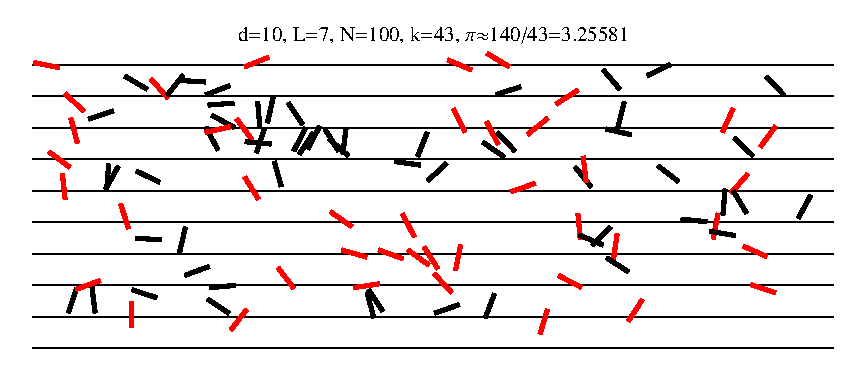
\includegraphics[height=0.3\textheight]{buffonsneedles.eps}
		\caption{Beispiel für eine Realisierung des Buffon--Nadel--Experiments mit 100 geworfenen Nadeln. Der erhaltene Schätzwert für $\pi$ ist bei so wenigen Nadeln nicht sehr genau.}
		\label{fig:buffon}
	\end{figure}
	
	\section{Das Integrationsproblem}\label{subsec:integrationsproblem}
	Betrachten wir das Integral
	\begin{equation}
		I=\int_\Omega f(x) d\mu(x),
		\label{eq:integration_problem}
	\end{equation}
	wobei $\Omega$ das Integrationsgebiet, $f : \Omega \to \mathbb{R}$ eine reellwertige Funktion und $\mu$ ein Ma"s auf $\Omega$ ist. Für die folgende Darstellung nehmen wir an, dass $$\Omega=[0,1]^d$$ der $d$--dimensionale Einheitswürfel und $I_d$ das zugehörige Integral ist.
	\subsection{Klassische numerische Quadraturverfahren}
	Die klassische numerische Herangehensweise (wenn keine analytische Lösung möglich oder praktikabel ist) sind {\em Tensor--Produkt--Verfahren}. Die Idee dabei ist, für jede Dimension ein eindimensionales Quadratur--Verfahren zu wählen (verschiedene oder das gleiche) und diese zu einem mehrdimensionalen Verfahren zu kombinieren. Ein eindimensionales Verfahren stellt eine gewichtete Summe von Funktionswerten an $M$ (vor dem Auswerten der Funktion) festgelegten Stützstellen dar:
	$${\tilde I}_1=\sum_{i=1}^M w_i\,f(x_i).$$
	Bekannte Vertreter dieser eindimensionalen Quadraturregeln sind z.B. die {\em Newton--Cotes}- und {\em Gauss--Legendre}--Verfahren. Ein hieraus konstruiertes Tensor--Produkt--Verfahren (wobei wir der Einfachheit halber für alle Dimensionen dasselbe eindimensionale Verfahren zugrundelegen) hat dann die Form:
	$${\tilde I}_d^{\,\text{TP}}=\sum_{i_1}^M\cdots\sum_{i_d}^M w_{i_1}w_{i_2}\cdots w_{i_d}f(x_{i_1},\cdots,x_{i_d}).$$
	Aus einem eindimensionalen Verfahren mit $M$ Stützstellen erhalten wir also ein $d$--dimensionales Verfahren mit $M^d$ Stützstellen (Siehe Abb. {\ref{fig:tensorproduct}}).
	\begin{figure}
		\centering
		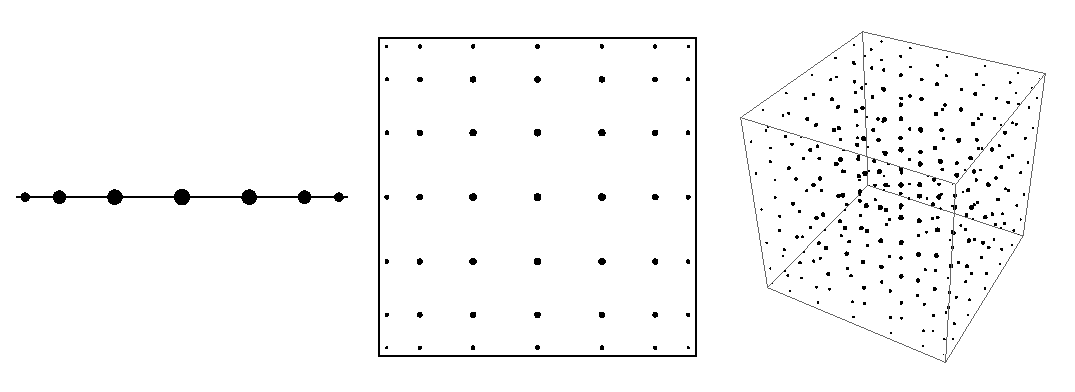
\includegraphics[height=0.25\textheight]{tensorproduct_quadrature.eps}
		\caption{Stützstellen eines 1D 7--Punkt--Gauss--Legendre--Verfahrens und entsprechender Tensor--Produkt--Verfahren für 2 bzw. 3 Dimensionen. Die Gewichte der Stützstellen sind durch ihre Grö"se kenntlich gemacht.}
		\label{fig:tensorproduct}
	\end{figure}
	
	\subsection{einfache Monte--Carlo--Integration}
	Bei der Monte--Carlo--Integration ziehen wir $N$ zufällige, gemä"s einer Wahrscheinlichkeitsdichte $p$ verteilte Stützstellen $[X_i|i\in\{1,\dots,N\}]$ in $\Omega$ und schätzen dann den Wert des Integrals (\ref{eq:integration_problem}) mit
	\begin{equation}
		{\tilde I}_d^{\,\text{MC}}=\frac{1}{N}\sum_{i=0}^{N-1} \frac{f(X_i)}{p(X_i)}
		\label{eq:mc_integral}
	\end{equation}
	ab. Im Falle unseres $d$--dimensionalen Einheitswürfels $\Omega=[0,1]^d$ können wir besipielsweise jede Stützstelle aus $d$ gleichförmig auf dem Einheitsintervall $[0,1]$ verteilten Zufallszahlen $U_i$ durch einfache Tupelbildung
	$$X_i:=(U_{d i},\dots,U_{d(i+1)-1})$$
	gewinnen. Aber auch für allgemeine Integrationsgebiete $\Omega$ kann das Verfahren genauso angewandt werden, solange ein passendes Integrationsma"s $\mu$ und ein Wahrscheinlichkeitsma"s $P$ existieren, so dass $$P(D)=\text{Pr}(x\in D)$$ für jede messbare Menge $D\subset\Omega$ gilt. Die entsprechende Wahrscheinlichkeitsdichte $p$ lässt sich mit Hilfe der {\em Radon--Nikodym--Ableitung} $$p(x)=\frac{dP}{d\mu}(x)$$
	einführen, wobei $p$ dann einfach eine Funktion ist, für die $$P(D)=\int_D p(x)d\mu(x)$$ gilt.
	Von der Erwartungstreue des Schätzers (\ref{eq:mc_integral}) für unser Integral (\ref{eq:integration_problem}) können wir uns mit \citep[][2.4]{Veach:1997p9136}
	\begin{align*}
		E[{\tilde I}_d^{\,\text{MC}}] &=E\left[\frac{1}{N}\sum_{i=0}^{N-1}\frac{f(X_i)}{p(X_i)}\right] \\
			&= \frac{1}{N}\sum_{i=0}^{N-1}E\left[\frac{f(X_i)}{p(X_i)}\right] \\
			&= \frac{1}{N}\sum_{i=0}^{N-1}\int_\Omega \frac{f(X_i)}{p(X_i)}p(X_i)\,d\mu(x) \\
			&= \int_\Omega f(x)\,d\mu(x)\\
			&= I
	\end{align*}
	leicht überzeugen.
	
	\subsection{Konvergenzraten}\label{subsec:integrationsproblem_comparison}
	Wir wollen nun die Konvergenzraten der Tensor--Produkt--Verfahren mit der Konvergenzrate des einfachen Monte--Carlo--Schätzers (\ref{eq:mc_integral}) vergleichen. Zur Konstruktion eines Vertreters der Tensor--Produkt--Verfahren verwenden wir beispielhaft das Newton--Cotes--Verfahren. In \citep[][3.1.4]{Stoer:2005p10586} wird als Ab\-schät\-zung für den Fehler eines Verfahrens $p$--ter Ordnung (d.h. ein Verfahren, das alle Polynome bis zum Grad $p$ exakt integriert) und Schrittweite $h(\approx\frac{b-a}{N}=\mathcal{O}(N^{-1}))$ der Stützstellen
	\begin{equation}
		\int_a^b P_n(x)-f(x)dx=h^{p+1}K f^{(p)}(\xi),\quad\xi\in(a,b)
		\label{eq:quadrature_error}
	\end{equation}
	angegeben, wobei $n$ die Anzahl der Stützstellen, $P_n$ das Interpolationspolynom für die Stützstellen und K eine Konstante ist. Gauss--Legendre--Verfahren sind von der Ordnung $2n-1$, d.h. die Konvergenzrate dieser $n$--Punkt--Formel ist demnach von der Grö"senordnung $\mathcal{O}(h^{2n})=\mathcal{O}(N^{-2n})$.\footnote{$N$ bezeichnet die Anzahl der Stützstellen für das gesamte Integrationsintervall. Der Schätzwert für das Integral wird dann durch $\frac{N}{n}$--maliges Anwenden der $n$--Punkt--Formel berechnet}
	Durch Bildung der entsprechenden $d$--dimensionalen Tensor--Produkt--Regel ändert sich die Konvergenzrate in Bezug auf die Schrittweite $h$ nicht. Da unsere $N$ Stützstellen sich nun aber auf ein $d$--dimensionales Gitter verteilen, teilt sich das Volumen unseres $d$--dimensionalen Einheitswürfels in $N$ Würfel mit einem Volumen von jeweils $h^d$ auf, d.h. für die Schrittweite folgt
	$$\mathcal{O}(1)=V=N h^d \Rightarrow h=\mathcal{O}\left(\left(\frac{1}{N}\right)^{1/d}\right)=\mathcal{O}\left(N^{-1/d}\right)$$	
	und damit für die Konvergenzrate in Bezug auf die Gesamtstützstellenzahl
	$$\mathcal{O}(h^{2n})=\mathcal{O}(N^{-2n/d}).$$
	Dies bedeutet, dass Tensor--Produktverfahren mit steigender Dimension des Integrationsgebietes an Effizienz verlieren. Bei hochdimensionalen Problemen kann dies kaum durch Verfahren höherer Ordnung ausgeglichen werden, da Verfahren höherer Ordnung, wie oben in (\ref{eq:quadrature_error}) zu sehen, auch grö"sere Anforderungen an die Glattheit der Funktion stellen. Au"serdem kann die exponentiell steigende Anzahl $N=n^d$ mindestens nötiger Funktionsaufrufe zu einem Problem werden. Der Effekt wird bei steigender Dimension und Ordnung des Verfahrens nur noch schlimmer, was ein Ausgleichen der schlechteren Konvergenzrate bei höheren Dimensionen durch Erhöhen der Ordnung des Verfahrens schnell praktisch unmöglich werden lässt. Dies wird häufig als {\em Curse~of~Dimensionality} (Fluch der Dimensionalität) bezeichnet.
	
	Bei der Monte--Carlo--Integration können wir die Konvergenzrate anhand der Varianz unseres Monte--Carlo--Schätzers (\ref{eq:mc_integral}) bestimmen \citep[][2.4.1]{Veach:1997p9136}. Nennen wir der Übersicht wegen
	$$Y_i=\frac{f(X_i)}{p(X_i)}$$
	und den MC--Schätzer mit $N$ gezogenenen Werten
	$$F_N=\frac{1}{N}\sum_{i=0}^{N-1} Y_i.$$
	Dann gilt für die Varianz eines beliebigen Samples
	\begin{equation}
		V[Y_i]=E[(Y_i-E[Y_i])^2]=E[Y_i^2]-E[Y_i]^2=\int_\Omega \frac{f(x)^2}{p(x)}d\mu(x)-I^2.
		\label{eq:mc_variance}
	\end{equation}
	Da die Werte unabhängig gezogen sind, gilt für die Varianz des Schätzer mit $N$ Werten
	$$V[F_N]=V\left[\frac{1}{N}\sum_{i=0}^{N-1}Y_i\right]=\frac{1}{N^2}V\left[\sum_{i=0}^{N-1}Y_i\right]=\frac{1}{N^2}\sum_{i=0}^{N-1}V[Y_i]=\frac{1}{N}V[Y_i],$$
	d.h. die Varianz des Schätzers sinkt invers mit der Anzahl $N$ an gezogenen Werten. Daraus folgt sofort die Standardabweichung
	\begin{equation}
		\sigma[F_N]=\frac{1}{\sqrt{N}}\sigma[Y_i],
		\label{eq:mc_standarddeviation}
	\end{equation}
	was einer Konvergenzrate von $\mathcal{O}(N^{-1/2})$ entspricht. Die Konvergenzrate des Monte--Carlo--Schätzers ist im Gegensatz zur Konvergenzrate der Tensor--Produkt--Verfahren also unabhängig von der Dimension des Integrationsgebietes, d.h. das Verfahren leidet {\em nicht} unter dem {\em Curse~of~Dimensionality}! Au"serdem mussten wir nirgendwo Bedingungen an die Glattheit der Funktion stellen, was bei Funktionen mit Diskontinuitäten von Vorteil ist.
	
	Zusammenfassend können wir also feststellen, dass Monte--Carlo--Integration bei hochdimensionalen Integrationsproblemen und Funktionen mit Diskontinuitäten klar gegenüber klassischen Tensor--Produktverfahren vorzuziehen ist. Für niedrigdimensionale ($d\lessapprox 7$) Gebiete mit glatten Integranden sind die klassischen Methoden hingegen besser geeignet.
	
	
	\section{Importance--Sampling}\label{subsec:importancesampling}
	Wir sind bei unserem MC--Schätzer (\ref{eq:mc_integral}) nicht darauf beschränkt eine gleich\-för\-mi\-ge Wahrscheinlichkeitsdichte $p$ zu wählen. Es kann die Effizienz des Verfahrens sogar beträchtlich verbessern, wenn wir eine geeignete Wahrscheinlichkeitsdichte $p$ wählen. Schauen wir uns daher die Formel (\ref{eq:mc_variance}) für die Varianz, die es zu minimieren gilt, nochmal an, um zu verstehen, was ``geeignet'' bedeutet. Nimmt die Wahrscheinlichkeitsdichte beispielsweise die ideale Form
	\begin{equation}
		p(x)=\frac{|f(x)|}{\int_\Omega |f(z)|d\mu(z)}
		\label{eq:ideal_importance_pdf}
	\end{equation}
	an, kann man mit der {\em Jensenschen~Ungleichung} zeigen, dass dann das Integral in (\ref{eq:mc_variance}) und damit die Varianz insgesamt minimal wird. Nimmt $f$ keine negativen Werte an, verschwindet die Varianz dieses Schätzers sogar, da in (\ref{eq:mc_integral}) dann nur noch über die konstante Lösung (in Form der Normierungskonstanten) gemittelt wird. Wenn wir das Normierungs--Integral im Nenner von (\ref{eq:ideal_importance_pdf}) lösen könnten, wäre allerdings auch die ursprüngliche Integration (\ref{eq:integration_problem}) kein Problem! Daher suchen wir in der Praxis nach einem $p$, das möglichst ähnlich zu $|f|$ und gleichzeitig normierbar ist.
	

		\chapter{Monte--Carlo--Markov--Chain--Verfahren}\label{chapter:mcmc}
	Im vorigen Abschnitt haben wir gesehen, wie mit unabhängig gezogenen identisch verteilten Samples der Erwartungswert einer Zufallsgröße abgeschätzt werden kann. In diesem Fall der numerische Wert eines Integrals. Insbesondere werden wir in Abschnitt \ref{sec:mc_radiativetransfer} sehen, wie wir damit den Wert einer Messung (im Sinne von Abschnitt \ref{sec:measurement_equation}) des Strahlungsintensitätsfeldes schätzen können. Beispielsweise kann dies ein Pixel eines (virtuellen) CCD--Sensors sein. Um ein Bild des kompletten CCD--Sensors zu erhalten würden wir daher jeden Pixelwert als eigenes Meßproblem auffassen und unabhängig voneinander lösen.
	
	Eine zweite Möglichkeit ist aber, die vielen kleinen Pixelsensoren zu einem großen Sensor zusammenzufassen, der die ganze CCD--Fläche abdeckt, und die gezogenen Werte nicht sofort zu einem Durchschnittswert über den ganzen Sensor zu mitteln, sondern vorher entsprechend der (bis dahin nicht vorhandenen) Pixelzugehörigkeit zu Klassen zusammenzufassen und in jeder Klasse (und damit in jedem Pixel) getrennt zu mitteln. Dies hat den Vorteil, dass wir durch den größeren Sensor schon vorher an allen Pixeln ``Interesse bekunden'' und damit mehr Möglichkeiten (in Form von Lichtpfaden) haben, ein beitragendes Sample zu erhalten. Berechnen wir hingegen alle Pixelsensor--Messwerte unabhängig voneinander, ist die Chance groß, bei der Messung eines Pixels genau die Pfade abzulehnen, die zum nächsten Pixel einen Beitrag geleistet hätten.
	
	Hieran zeigt sich, dass wir häufig nicht an einzelnen, für sich alleine stehenden Messwerten interessiert sind, sondern an der Verteilung der Samples über verschiedene Klassen, z.B. die Verteilung der Photonen auf einem CCD--Sensor oder die Verteilung von Photonen über die verschiedenen Wellenlängen in einem Spektrum. In all diesen Fällen lohnt es sich, die Messung mit dem größtmöglichen Sensor vorzunehmen und die Klasseneinteilung und Mittelung danach vorzunehmen.

	In vielen Fällen in denen solch eine nachgezogene Klasseneinteilung sinnvoll ist, ist die relative Verteilung der Samples über die Klassen wichtiger als die absoluten Messwerte für die einzelnen Klassen. Bei manchen Problemen, beispielsweise bei der Schätzung eines Spektrums, sind wir sogar nur an diesen relativen Häufigkeiten der Samples interessiert und die absoluten Messwerte sind nicht relevant. In solch einem Fall ist die Normierung der Wahrscheinlichkeitsverteilung, aus der die Samples gezogen werden nicht nötig. Hier reicht es aus, über ein Verfahren zu verfügen, das Samples aus der Verteilung ziehen kann, ohne ihre Wahrscheinlichkeiten mitzuliefern.
	
	Genau dies leisten sogenannte {\em Mon\-te--Car\-lo--Mar\-kov--Chain--Ver\-fahr\-en} (MCMC--Verfahren). Sie stellen Verfahren dar, um aus einem Zustandsraum $\Omega$ gemäß einer gegebenen Wahrscheinlichkeitsdichte $f$ verteilte Werte zu ziehen. Dies wird durch die Konstruktion eines Zufallspfads ({\em random~walk}) im Zustandsraum, dirigiert durch eine Markov--Kette, erreicht. Dabei muß sichergestellt werden, dass die so erzeugten Werte auch gemäß $f$ verteilt sind und insbesondere jeder Punkt im Zustandsraum, auf dem $f$ nicht verschwindet, auch erreicht werden kann.
	
	Wie im nächsten Abschnitt gezeigt wird, ist dies mit erstaunlich wenig Aufwand möglich. Selbst wenn doch eine Normierung nötig ist, kann es sinnvoll sein, die Normierung mit einem klassischen Monte--Carlo--Integrations--Verfahren über den Gesamtsensor zu bestimmen und die Verteilung des Samples über die Klassen innerhalb des Sensors mit einem MCMC--Verfahren zu ermitteln.
	
	Die Kombination aus Vielseitigkeit, Mächtigkeit und Einfachheit hat MCMC--Verfahren in vielen Bereichen\footnote{Beispiele finden sich u.a. in der statistischen Physik, in der Finanzmathematik und zur Berechnung von A--posteriori--Wahrscheinlichkeiten in der Bayes'schen Statistik \citep{Geweke:1989p10465}, z.B. mit Anwendungen in der Bioinformatik und Medizin. Weitere interessante und ungewöhnliche Anwendungen finden sich in \citep{Diaconis:2009p4122}} zu einem Hauptverfahrensbestandteil gemacht.
	
	
	\section{Metropolis--Hastings--Algorithmus}
	Unter den MCMC--Verfahren ist eines der bekanntesten der {\em Metropolis--Hastings--Algorithmus} (MH), der durch eine Arbeit in der statistischen Physik von \citet{Metropolis:1953p3364} in einer einfachen Form vorgestellt und später durch \citet{Hastings:1970p3387} verallgemeinert wurde.

	Beim MH--Algorithmus ziehen wir aus einem Zustandsraum $\Omega$ Elemente $x \in \Omega$ gemäß der (nicht notwendigerweise normierten!) Wahrscheinlichkeitsdichte $f : \Omega \rightarrow \mathbb{R}_{\geq 0}$. Die Elemente werden dabei mit einem Zufallspfad durch den Zustandsraum generiert. Wir verändern dazu den aktuellen Zustand $x$ nach einem frei wählbaren Schema (im Folgenden Mutation genannt) in einen neuen Zustand $x'$.
	Dabei stellen wir folgende Bedingungen an eine Mutation:
	\begin{itemize}
		\item{wenn der übergang von Zustand $x$ nach $x'$ möglich ist, muss auch der übergang zurück von $x'$ nach $x$ möglich sein}
		\item{es muss jeder Zustand $x \in \Omega$ durch eine Kette von übergängen erreichbar sein (Ergodizität)}
		\item{Die übergangswahrscheinlichkeit $T(x'|x)$ durch unser Mutations--Schema von Zustand $x$ zum Zustand $x'$ zu kommen muss für gegebenes $x$ und $x'$ berechenbar sein}
	\end{itemize}
	Mutationen sind also, etwas formaler formuliert, bedingte Wahrscheinlichkeitsverteilungen, die durch das Herkunftselement parametrisiert sind, nicht normiert sein müssen und für die
	$$\forall x,x'\in\Omega : \quad T(x'|x)>0 \Leftrightarrow T(x|x')>0$$
	wahr ist. Hierin können wir eine Parallele zum {\em Importance Sampling} aus Abschnitt \ref{subsec:importancesampling} entdecken, bei dem wir auch die A--priori--Wahr\-schein\-lich\-keits\-ver\-tei\-lung, aus der die Werte gezogen werden, selber wählen können ohne das Ergebnis der Integration zu verfälschen. Während wir uns beim Importance Sampling allerdings für eine einzige Verteilung zur Generierung der gesamten Stichprobe entscheiden müssen, haben wir beim {\em MH--Algorithmus} die Möglichkeit, für jeden aktuellen Zustand eine eigene Verteilung festzulegen, aus der ein Vorschlag für den neuen Zustand gezogen wird.
	Das bedeutet, Mutationen können (und sollten) für effizientes und verlässliches Verhalten an das spezifische Samplingproblem angepasst werden, indem die Eigenschaften der interessierenden Wahrscheinlichkeitsdichte $f$ und des Zustandsraumes $\Omega$ miteinbezogen werden. Sind beispielsweise exakte oder näherungsweise gültige Invarianten von $f$ bezüglich seiner Zustandsraumkoordinaten bekannt, können diese genutzt werden, um Samples ähnlicher Wahrscheinlichkeitsdichte aber gering korrelierter Zustandsraumkoordinaten zu ziehen.
	
		
	\paragraph{Detailed Balance:}
	Da die Mutation, mit der wir den neuen Zustand generieren, nichts mit der Wahrscheinlichkeitsdichte $f$ zu tun haben muss, brauchen wir eine Möglichkeit die Verteilung der Zustände gemäß $f$ trotzdem sicherzustellen.
	
	Betrachten wir eine große Zahl von gleichartigen aber unabhängigen Markov--Ketten, die alle mit einer gewissen Wahrscheinlichkeit $p(x'|x)$ vom Zustand $x$ in den Zustand $x'$ übergehen und mitteln über die aktuellen Zustände aller Markov--Ketten. Dann ist eine Möglichkeit eine stationäre Zustandsdichte $f$ zu erreichen, zu verlangen, dass
	\begin{equation}
		\forall x,x' \in \Omega :\quad f(x)p(x'|x) = f(x')p(x|x')
		\label{eq:dynamic_equlibrium}
	\end{equation}
	({\em =Detailed Balance}) gilt, d.h. dass sich die übergangsraten zwischen zwei beliebigen Zuständen im dynamischen Gleichgewicht befinden.
	Da $T$ die übergangswahrscheinlichkeiten aber schon festlegt, behalten wir uns das Recht vor, einen durch Ziehen aus $T$ vorgeschlagenen Zustandsübergang nur mit der Wahrscheinlichkeit $a(x'|x)$ anzunehmen und ansonsten abzulehnen,	um {\em Detailed Balance} sicherstellen zu können:
	\begin{equation}
		p(x'|x) = T(x'|x)a(x'|x)
		\label{eq:acceptance_prob_intro}
	\end{equation}
	\begin{equation}
		(\ref{eq:dynamic_equlibrium}) \stackrel{(\ref{eq:acceptance_prob_intro})}{\Longrightarrow}
		\forall x,x' \in \Omega :\quad f(x)T(x'|x)a(x'|x) = f(x')T(x|x')a(x|x')
		\label{eq:detailedbalance}
	\end{equation}
	Dies lässt noch immer verschiedene Möglichkeiten zu, die Akzeptanzwahrscheinlichkeit zu bestimmen. Eine effiziente und dadurch beliebte Wahl ist dabei Folgende: ist $f(x')>f(x)$ nehmen wir den neuen Zustand auf jeden Fall an, ansonsten mit der Wahrscheinlichkeit $(f(x')T(x|x'))/(f(x)T(x'|x))$. Dies lässt sich zusammenfassen zu
	\begin{equation}
		a(x'|x)=\text{min}\left(1,\frac{f(x')T(x|x')}{f(x)T(x'|x)}\right)
		\label{eq:acceptanceratio}
	\end{equation}
	Diese Wahl der Akzeptanzwahrscheinlichkeit erfüllt die Detailed--Balance--Bedingung (\ref{eq:detailedbalance}).
	
	
	
	\paragraph{Pseudocode:}
	In Pseudocode sieht der Algorithmus dann wie folgt aus:
	\begin{algorithmic}
		\STATE $x_1 \leftarrow$ Anfangszustand
		\FOR{$i=1$ to $N$}
			\STATE $x'\leftarrow$ ziehe Wert gemäß $T(x'|x_i)$
			\STATE $a(x'|x_i) \leftarrow \text{min}\left(1, \frac{f(x')T(x|x')}{f(x)T(x'|x)}\right)$
			\STATE $u\leftarrow$ Zufallszahl aus $[0,1]$
			\IF{$u < a(x'|x_i)$}	\STATE $x_{i+1} \leftarrow x'$
			\ELSE	\STATE $x_{i+1} \leftarrow x_i$
			\ENDIF
	  \ENDFOR
	\end{algorithmic}
	Als Ergebnis erhalten wir eine Liste von Werten, die gemäß $f$ verteilt sind.
	Die Tatsache, dass die Normierung von $f$ für die Funktion des Verfahrens nicht notwendig ist, kann einerseits von Vorteil sein, und bei bestimmten Problemen die effiziente Generierung einer Stichprobe erst möglich machen. Sie bedeutet allerdings, dass wir uns bei Bedarf eine Normierung auf andere Weise beschaffen müssen, da die gezogenen Werte ebenfalls nicht normiert sind. Die Werte sind außerdem nicht unabhängig, sondern im Gegenteil häufig stark korreliert.

	\paragraph{Konvergenz:}Bei klassischer Monte--Carlo--Integration hatten wir in Abschnitt \ref{subsec:integrationsproblem_comparison} gezeigt, dass bei einer Standard--Abweichung eines Wertes von $$\sigma^*:=\sigma\left[\frac{f(X_i)}{p(X_i)}\right]$$ die Standard--Abweichung des Mittelwertes von N unabhängig gezogenen Werten $\sigma^*/\sqrt{N}$ beträgt. Sind die Werte hingegen korreliert, gilt für die Standard--Abweichung des Mittelwertes die Abschätzung \citep[siehe][VII.\;\S3(8)]{Renyi:1964p10655}
	$$\sigma\leq \sigma^*\sqrt{\frac{1+2\sum_{i=1}^N R(i)}{N}},$$
	wobei $R(|j-i|)\leq 1$ eine obere Schranke für die Korrelation zwischen $f(X_i)/p(X_i)$ und $f(X_j)/p(X_j)$ ist.
	Eine große Korrelation kann sich also negativ auf die Konvergenzrate des Mittelwertes (und anderer statistischer Kenngrößen) auswirken. Daher gilt es bei der Konstruktion einer Mutation zwei Aspekte gegeneinander abzuwägen: einerseits ist es wünschenswert in einem Mutationsschritt möglichst ``große Schritte'' zu machen um die Korrelation der Werte kleinzuhalten, andererseits ist es in selten gezogenen Bereichen mit hohem Beitrag wünschenswert kleine Schritte zu machen, um diesen Bereich gut abzudecken. Während ersteres Verfahren meist mit einer kleinen Akzeptanzwahrscheinlichkeit einhergeht, führen kleine Mutationen tendenziell zu hohen Akzeptanzwahrscheinlichkeiten. Beide ziehen aber in zu extremer Form hohe Korrelation der Samples nach sich, bei zu großen Schritten aufgrund der geringen Akzeptanzwahrscheinlichkeit und daher mehrfacher Gewichtung desselben Samples, bei zu kleinen Schritten aufgrund der großen ähnlichkeit der vorgeschlagenen Samples. Daher sind sowohl zu hohe als auch zu kleine Akzeptanzwahrscheinlichkeiten meistens ein Zeichen suboptimalen Samplings. In \citep{Roberts:1997p5198} wird zur Steuerung der Mutationsstärke für die Akzeptanzwahrscheinlichkeit ein anzustrebender Wert von $\approx 0.23$ bei hochdimensionalen Problemen empfohlen.

	
	
	\section{Robuster Metropolis--Hastings--Algorithmus}
	Wir haben in Abschnitt \ref{subsec:importancesampling} festgestellt, dass die Effizienz des einfachen Monte--Carlo--Schätzers erheblich verbessert werden kann, wenn für {\em Importance Sampling} eine geeignete A--priori--Wahrscheinlichkeitsdichte $p$ bekannt und samplebar ist. Parallel dazu haben wir im vorigen Abschnitt gesehen, dass es auch für ein effizientes Funktionieren des {\em Metropolis--Hastings--Algorithmus} wichtig ist, die Mutationen an das Problem anzupassen. Meistens geschieht dies dadurch, dass verschiedene Mutationen erdacht werden, die jeweils in einem Teilbereich des Zustandsraumes effizient sind. Als Beispiel könnten wir bei jedem neuen Sample zufällig zwischen einer Mutation, die große Schritte macht und einer anderen, die nur kleine Veränderungen vornimmt, wählen. Zur Generierung eines neuen Samples wird dann zufällig eine der Mutationen ausgewählt und auf das letzte Sample angewandt.
	
	In \citep{Kelemen:2002p8514} wird hingegen eine elegante Variante des Metropolis--Algorithmus vorgeschlagen, die im Wesentlichen mit nur einer Mutation auskommt und trotzdem über die gewünschte Eigenschaft verfügt sich an die lokalen Gegebenheiten anpassen zu können. Dem Verfahren liegt dabei folgende Idee zugrunde: Wenn es möglich wäre den Zustandsraum $\Omega$ und die Wahrscheinlichkeitsdichte $f$ so zu transformieren, 	dass $f$ gleichmäßiger verteilt ist, dann würde es ausreichen eine einzige Mutation auf diesem transformierten Zustandsraum operieren zu lassen. Dann würden Teilgebiete von $\Omega$ mit hohen Spitzenwerten in $f$ zu größeren Gebieten ``gedehnt'', und größere Teilgebiete mit kleinen $f$--Werten ``gestaucht'' werden, und $f$ dadurch gleichmäßiger werden lassen. Eine Mutation, die auf dem transformierten Zustandsraum operiert, würde dann automatisch dort kleinere Schritte machen, wo $f$ plötzlich groß wird und größere Schritte dort, wo $f$ flach und klein ist.
	
	Solch eine Transformation bekommen wir ``geschenkt'', falls wir Punkte im Zustandsraum mittels {\em Importance Sampling} generieren, was bei komplizierteren Problemen (wie dem Strahlungstransportproblem) ohnehin meist der Fall ist (siehe Abschnitt \ref{sec:mc_radiativetransfer}). Schauen wir uns dazu als Beispiel das Integrationsproblem
	\begin{equation}
		I=\int_\Omega f(x) d\mu(x)\approx \frac{1}{N}\sum_{i=0}^{N-1} \frac{f(X_i)}{p(X_i)}
		\label{eq:transformedintegral1}
	\end{equation}
	aus Abschnitt \ref{subsec:integrationsproblem} an. Die Samples aus $p$ werden zumeist durch Transformation gleichförmig verteilter Zufallszahlen aus dem Einheitsinterval $[0,1]$ generiert. Daher können wir eine gezogene Konfiguration von (potentiell unendlich vielen) Zufallszahlen als Koordinaten im unendlichdimensionalen Einheitswürfel $[0,1]^\infty$ auffassen. Nennen wir diesen den {\em primären Sample--Raum} $\mathcal{U}$ und bezeichnen die Transformation vom primären Sample--Raum in unseren Zustandsraum als
	$$S : \mathcal{U} \to \Omega\,,\quad x=S(u).$$
	Dann können wir unser Integral (\ref{eq:transformedintegral1}) auch als transformiertes Integral
	$$I=\int_\mathcal{U} f(S(u)) \left|\frac{dS(u)}{du}\right|du=\int_\mathcal{U} \frac{f(S(u))}{p_S(u)}du$$
	schreiben, wobei
	$$\left|\frac{dS(u)}{du}\right|=\frac{1}{p_S(u)}$$
	die Jacobi--Determinante der Abbildung $S$ ist. Bildlich gesprochen drückt die Jacobi--Determinante die lokale Dehnung bzw. Stauchung einer Transformation zwischen zwei Räumen aus. Wenn $u$ also eine gleichmäßig verteilte Zufallsvariable darstellt, ist $p_S(u)$ die Wahrscheinlichkeitsdichte von $x=S(u)$. Da $S$ die Zufallszahlen aus dem primären Sample--Raum vermehrt auf Punkte im Zustandsraum $\Omega$ mit hohem $f$ abbildet, variiert unser neuer Integrand $f(S(u))/p_S(u)$ nicht mehr so stark, ist also flacher geworden. Unsere Mutation, die nun im primären Sample--Raum mit konstanter durchschnittlicher Schrittweite agiert, passt sich dadurch automatisch an die lokalen Gegebenheiten an, d.h. sie macht kleine Schritte in $\Omega$ wenn $f$ groß ist, und größere Schritte, wenn $f$ klein ist. Die Effizienz des Verfahrens können wir nun also dadurch verbessern, dass wir das Importance Sampling besser auf das Problem abstimmen. Die Tatsache, dass nun die Mutationen indirekt durch die Transformation vom primären Sampleraum in den Zustandsraum definiert werden, erhöht auch die Modularität und damit die Wiederverwendbarkeit des Algorithmus in Form eines Computerprogramms (siehe dazu Abschnitt \ref{cha:program_description} für Details).

	Zum Vorschlagen neuer Samples benutzen wir zwei Mutationen. Zum einen können durch Wählen eines neuen Satzes gleichförmig verteilter Zufallszahlen aus $\mathcal{U}$ {\em frische} Samples vorgeschlagen werden. Dies stellt sicher, dass jeder Punkt in $\mathcal{U}$ bzw. $\Omega$ erreicht werden kann und stellt so die Ergodizität des Verfahrens sicher und macht es robuster. Bei sehr schwierigen Sampling--Problemen verhält sich das Verfahren dann schlimmstenfalls wie ein klassischer Monte--Carlo--Sampler mit Importance Sampling, bei dem jedes Sample unabhängig gezogen wird.
	Die andere Mutation addiert zu den vorhandenen Koordinaten des aktuellen Samples aus $\mathcal{U}$ jeweils eine kleine Störung, so dass jede Koordinate sich ändert aber mit großer Wahrscheinlichkeit in der Nähe der alten Koordinate landet. Die Störung ist dabei symmetrisch um Null, d.h. es ist gleichwahrscheinlich einen Versatz $\Delta u$ zu ziehen wie $-\Delta u$. Die Koordinaten werden dabei als periodisch angesehen, d.h. bei überschreiten des rechten Randes von $[0,1]$ wird der ganzzahlige Teil abgeschnitten um wieder im Einheitsintervall zu landen. Dies birgt einen Effizienz--Vorteil, da die Symmetrie der Störung bedeutet, dass für die Übergangswahrscheinlichkeiten
	\begin{equation}
	  T(u'|u)=T(u|u')
	  \label{eq:symmetric_transitionprob}
	\end{equation}
	gilt und sie sich daher in der Berechnung der Akzeptanzwahrscheinlichkeit
	$$a(u'|u)=\text{min}\left(1,\frac{f(S(u'))T(u|u')}{f(S(u))T(u'|u)}\right)\stackrel{(\ref{eq:symmetric_transitionprob})}{=}\text{min}\left(1,\frac{f(S(u'))}{f(S(u))}\right)$$
	herauskürzt. Im Falle der {\em frischen Mutation} kürzt sich die Übergangswahrscheinlichkeit $T$ ebenfalls heraus, da aus $\mathcal{U}$ gleichmäßig gezogen wird.
	In Pseudocode sieht der Algorithmus dann wie folgt aus:
	\begin{algorithmic}
		\STATE $u \leftarrow$ Anfangszustand
		\STATE $x_1 \leftarrow S(u)$
		\FOR{$i=1$ to $N$}
			\STATE $r\leftarrow$ Zufallszahl aus $[0,1]$
			\IF[Mutation schlägt frisches Sample vor]{$r < p_\text{fresh}$}
						\STATE $T \leftarrow T_\text{fresh}$
			\ELSE[Mutation schlägt leicht abgewandeltes Sample vor]	\STATE $T \leftarrow T_\text{perturb}$
			\ENDIF
			\STATE $u'\leftarrow$ ziehe Wert gemäß $T(u'|u)$
			\STATE $x' \leftarrow S(u')$
			\STATE $a(u'|u) \leftarrow \text{min}\left(1,\frac{f(x')}{f(x_i)}\right)$
			\STATE $r\leftarrow$ Zufallszahl aus $[0,1]$
			\IF{$r < a(u'|u)$}
			  \STATE $x_{i+1} \leftarrow x'$
			  \STATE $u \leftarrow u'$
			\ELSE	\STATE $x_{i+1} \leftarrow x_i$
			\ENDIF
	  \ENDFOR
	\end{algorithmic}


		\chapter{Monte--Carlo--Strahlungstransport}\label{sec:mc_radiativetransfer}
	In diesem Abschnitt wollen wir die Theorie zum Strahlungstransport aus Abschnitt \ref{sec:radiative_transfer} und \ref{chapter:path_radiative_transfer} mit den Integrations- und Samplingverfahren aus den Abschnitten \ref{chapter:mc_integration} und \ref{chapter:mcmc} zusammenf"uhren, um zu zeigen wie konkrete Verfahren zur L"osung des Strahlungstransportproblems konstruiert werden k"onnen.
	\section{Strahlungstransport als Integrationsproblem}
	In Abschnitt \ref{sec:neumann_elimination} haben wir gesehen, da"s sich L"osungen des Strahlungstransportproblems in Form von Messungen des Strahlungsintensit"atsfeldes als Integration der Beitragsmessfunktion $f$ "uber den Raum aller m"oglichen Lichtpfade $\Omega$ darstellen lassen:
	\begin{equation}
		M=\int_\Omega f({\overline x})d\mu({\overline x}).
		\label{eq:mcrad_measurement_integral}
	\end{equation}
	Wir haben dann in Abschnitt \ref{chapter:mc_integration} Monte--Carlo--Integration als Verfahren zur numerischen L"osung von allgemeinen Integrationsproblemen kennengelernt. Schliesslich haben wir mit den MCMC--Verfahren eine Methode behandelt, um Messsprobleme, bei denen wir besonders an der Verteilung der Werte "uber verschiedene Bereiche des Sensors interessiert sind, effizient l"osen zu k"onnen.
	
	Wir wollen nun diese vorgestellten Techniken speziell auf das in der L"osung des Strahlungstransportproblems auftretende Integral (\ref{eq:mcrad_measurement_integral}) anwenden. Da wir schon viel der dazu n"otigen Techniken in den vorangegangenen Abschnitten allgemein behandelt haben, fehlt nun f"ur ein komplettes Verfahren nur eine Methode, die Photonenpfade zu generieren und die entsprechende Wahrscheinlichkeitsdichte $p$, die jedem Pfad ${\overline x}\in\Omega$ eine differentielle Wahrscheinlichkeit zuweist von dem Verfahren erzeugt worden zu sein.
	
	\section{Pfadgenerierung}
	\subsection{Definition der Pfadwahrscheinlichkeitsdichte}
	In Abschnitt \ref{sec:neumann_elimination} hatten wir f"ur Pfade der L"ange $k$ das Integrationsma"s $$d\mu_k=d\nu d\location{r}_0\cdots d\location{r}_{k+1}$$ eingef"uhrt, das einfach das Produktma"s aus den Volumenma"sen $d\location{r}_i$ der beteiligten Pfadpunkte sowie dem Integrationsma"s $d\nu$ f"ur die Frequenz des Lichtes ist. Die dazugeh"orige Wahrscheinlichkeitsdichte ist durch die {\em Radon--Nikodym--Ableitung} mit
	$$p_k(\nu,\location{r}_0\cdots \location{r}_{k+1})=\frac{dP}{d\nu}(\nu)\frac{dP}{d\location{r}_0}(\location{r}_0)\cdots\frac{dP}{d\location{r}_{k+1}}(\location{r}_{k+1})$$
	gegeben. Jeder der Faktoren stellt dabei eine Wahrscheinlichkeitsdichte dar ein Photon der Frequenz $\nu$ zu generieren bzw. den $i$-ten Punkt des Pfades am Ort $\location{r}_i$ vorzufinden. Jede Wahrscheinlichkeitsdichte ist f"ur sich genommen normiert, d.h. es gilt
	$$\int_{\mathbb{R}_+} \frac{dP}{d\nu}(\nu) d\nu=1,\qquad \int_{\mathbb{R}^3} \frac{dP}{d\location{r}_i}(\location{r}_i) d\location{r}_i=1$$
	f"ur alle $i\in\{0,1,\dots,k,k+1\}$. Zus"atzlich m"ussen wir aber noch die Wahl der Pfadl"ange selbst durch eine diskrete Wahrschinlichkeitsverteilung
	$$P_L(i)=\text{Pr}(k=i),\quad\sum_{k=0}^\infty P_L(k)=1,\quad k\in\{0,1,2,\cdots\}$$ ber"ucksichtigen, die angibt wie gro"s die Wahrscheinlichkeit ist, mit unserer Pfadgenerierungsmethode einen Pfad mit $k$ Streupunkten zu generieren. Die Wahrscheinlichkeitsdichte f"ur einen beliebigen Pfad lautet dann
	\begin{align}
		p(\nu,\location{r}_0\cdots \location{r}_{k+1})&=P_L(k)p_k(\nu,\location{r}_0\cdots \location{r}_{k+1}) \nonumber\\
		&=P_L(k)\frac{dP}{d\nu}(\nu)\frac{dP}{d\location{r}_0}(\location{r}_0)\cdots\frac{dP}{d\location{r}_{k+1}}(\location{r}_{k+1}).
		\label{eq:path_probabilitydensity}
	\end{align}
	Die Wahrscheinlichkeitsdichte f"ur Photonenpfade ist also ein Produkt aus den Wahrscheinlichkeitsdichten f"ur die kontinuierlichen Gr"o"sen in Form der Photonenfrequenz und der Pfadpunkte sowie der diskreten Wahrscheinlichkeitsverteilung zur Wahl der Anzahl an Streupunkten.
	
	Jede Pfadgenerierungsmethode, die wir im Folgenden entwickeln, bedarf einer solchen Wahrscheinlichkeitsdichte, d.h. wir m"ussen in der Lage sein, die Wahrscheinlichkeitsdichte auf die Form (\ref{eq:path_probabilitydensity}) zur"uckzuf"uhren.
	
	\subsection{Naive Pfadgenerierung}
	An der Produktform von (\ref{eq:path_probabilitydensity}) sehen wir, da"s die Wahl der Anzahl an Streupunkten, der Photonenfrequenz und der Pfadpunkte unabh"angig voneinander getroffen werden k"onnen (wobei nat"urlich die Anzahl an Faktoren f"ur die Pfadpunkte von der Wahl der Pfadl"ange abh"angt). Daher best"ande der naheliegendste Ansatz Pfade zu generieren darin, f"ur jeden der Faktoren eine statische Wahrscheinlichkeitsverteilung festzulegen, aus der wir dann unabh"angig voneinander die einzelnen Pfadbestandteile ziehen. Die k"onnen wir dann anschliessend zu einem Pfad zusammensetzen. Der Pseudocode k"onnte beispielsweise so aussehen:
	\begin{algorithmic}
		\STATE $\nu \leftarrow$ ziehe Wert gleichf"ormig aus $[\nu_\text{min},\nu_\text{max}]$
		\STATE $k \leftarrow$ ziehe Wert aus Poissonverteilung mit Erwartungswert $2.5$
		\STATE $\location{r}_0 \leftarrow$ ziehe Ort gleichf"ormig aus der Lichtquelle
		\STATE $\location{r}_{k+1} \leftarrow$ ziehe Ort gleichf"ormig aus dem Sensor
		\FOR{$i=1$ to $k$}
			\STATE $\location{r}_i \leftarrow$ ziehe Ort gleichf"ormig aus dem Streuvolumen
	  \ENDFOR
	  \RETURN $(\nu,\location{r}_0\location{r}_1\cdots\location{r}_{k+1})$
	\end{algorithmic}
	Auch wenn diese Methode einfach zu verstehen und einfach zu implementieren ist, ist sie fast immer sehr ineffizient, da sie bis auf die Geometrie der Lichtquelle, des Sensors und des Streuvolumens keinerlei weitere Informationen einbezieht, was in der Praxis bedeutet, da"s der "uberwiegende Teil der generierten Pfade in die {\em Messbeitragsfunktion} $f$ (\ref{eq:mcf}) eingestzt null oder nur einen sehr kleinen Wert und damit nur einen sehr geringen Beitrag zum Messwert liefert.
	Dies liegt daran, da"s $f$ aus vielen Faktoren besteht, und es daher ausreicht wenn einer von ihnen verschwindet oder sehr klein wird, um den Beitrag des ganzen Pfades verschwinden zu lassen.

	Wir sollten also versuchen Pfade so zu erzeugen, da"s m"oglichst viele der Faktoren in $f$ gro"s werden und die Chance gering ist, da"s einer von ihnen null wird.

	\subsection{Raycasting}
	Eine M"oglichkeit dazu, die zudem auch physikalisch motiviert ist, besteht darin die Punkte nicht unabh"angig voneinander, sondern stattdessen bei einem Ende des Pfades beginnend, rekursiv vom jeweils letzten generierten Punkt aus zu ziehen. Dies wird auch als {\em Raycasting} bezeichnet.
	
	Genauer bedeutet dies, da"s wir ausgehend vom letzten generierten Punkt $\location{r}_{i-1}$ aus, zuerst eine Richtung $\omega$ und dann eine Entfernung $s$ aus entsprechenden Wahrscheinlichkeitsdichten (PDF) ziehen, die angibt wie weit wir uns von $\location{r}_{i-1}$ in Richtung $\omega$ bewegen. Der n"achste Punkt hat dann die Koordinaten
	$$\location{r}_i=\location{r}_{i-1}+s\,\omega$$
	Die "aquivalente Wahrscheinlichkeitsdichte bezogen auf's Volumenma"s von $\location{r}_i$ ist dann
	\begin{align*}
		\frac{\text{d}P}{\text{d}\location{r}_i}(\location{r}_i) &= \frac{\text{d}P}{s^2 \text{d}\omega\text{d}s}(\location{r}_i) \\
		&= \underbrace{\frac{1}{\|\location{r}_i - \location{r}_{i-1}\|^2}}_{\text{geometrische}\atop\text{Verd"unnung}} \cdot\underbrace{\frac{\text{d}P}{\text{d}\omega}(\location{r}_i)}_{\text{Richtungs--PDF}} \cdot \underbrace{\frac{\text{d}P}{\text{d}s}(\location{r}_i)}_{\text{Entfernungs--PDF}}
	\end{align*}
	Als Richtungs--PDF bietet sich dabei die Phasenfunktion des Materials an
	\begin{equation}
		\frac{\text{d}P}{\text{d}\omega}(\location{r}_i) = k(\location{r}_{i-2}\rightarrow\location{r}_{i-1} \rightarrow\location{r}_i).
		\label{eq:direction_pdf}
	\end{equation}
	F"ur die Entfernungs--PDF ergibt sich bei gleichf"ormig zuf"allig gezogenem Anteil durch Extinktion verlorener Strahlung $\eta$
	\begin{align}
		\eta &= \underbrace{1-e^{-\int_0^s \xi(\location{r}+s\,\omega)\text{d}s}}_\text{CDF} \,,\quad \eta \in (0,1) \nonumber \\
		\Rightarrow \frac{\text{d}P}{\text{d}s}(\location{r}_i) &= \dds \left(1-e^{-\int_0^s \xi(\location{r}+s\,\omega)\text{d}s}\right) \nonumber \\
		&= \xi(\location{r}+s\,\omega) e^{-\int_0^s \xi(\location{r}+s\,\omega)\text{d}s}
		\label{eq:distance_pdf}
	\end{align}
	
	Mit dieser Methode l"asst sich der Zufallspfad eines Photons in ``nat"urlicher Weise'' (d.h. mit gleicher Wahrscheinlichkeitsverteilung) nachvollziehen wenn wir bei einem zuf"allig aus der Lichtquelle gezogenen Punkt starten und von dort aus rekursiv Streupunkte und zum Schlu"s den Sensorpunkt ziehen. Wir haben aber z.B. auch die Freiheit die Pfadgenerierung bei einem zuf"allig gezogenen Sensorpunkt zu beginnen und uns ``r"uckw"arts'' zur Lichtquelle vorzuarbeiten.
	\subsection{Distanzsampler}
	TODO: uniform depth sampler, uniform attenuation sampler, enforced uniform attenuation sampler
	
	TODO: Pfadgenerierung, Sch"atzer
	
		\chapter{Programmbeschreibung}\label{cha:program_description}
	In diesem Abschnitt soll eine Implementation einiger der in den bisherigen Abschnitten vorgestellten Ideen in Form des Computerprogramms \texttt{PIRaTE} (=\texttt{P}ath \texttt{I}ntegral \texttt{Ra}diative \texttt{T}ransfer with \texttt{E}ase) vorgestellt werden. Dabei soll zum einen ein Überblick über das Programm durch eine abstrakte Modulbeschreibung gegeben werden. Zum anderen sollen aber auch interessante Implementationsdetails herausgegriffen und vorgestellt werden.
	
	%TODO: Programmbeschreibung in Worten bzw. Pseudocode, Modulbeschreibung, Details in evtl. Anhang auslagern, Erhöhte Modularität beim robusten MH-Algo durch feste Mutationen, die über die Sample--Generierungsmethode adaptiv angepasst werden.
	
	%\section{Allgemeines}
	\section{Programmiersprache}
	\pirate ist in der rein funktionalen Programmiersprache {\em Haskell} geschrieben. Funktionale Programmiersprachen bauen auf der Idee auf, Programme als Aneinanderreihung vieler kleiner Funktionen darzustellen, von denen jede Funktion eine bestimmte Aufgabe erfüllt. Das Ergebnis einer Funktion hängt dabei nur von den Eingabeparametern ab, d.h. gleiche Eingabewerte führen immer zum gleichen Rückgabewert, was genau der mathematischen Idee einer Funktion entspricht. Funktionen sind somit nebeneffektfrei, d.h. sie können weder auf Zustände (wie z.B. die Uhrzeit oder der Inhalt einer Datei) ausserhalb ihrer Eingabeparameter zurückgreifen, noch kann die Funktion selber, vom Rückgabewert abgesehen, Einfluß auf den ``Zustand der Welt'' (d.h. den Inhalt von Dateien oder eine Ausgabe auf dem Bildschirm) nehmen.
	
	Da der Sinn eines Programmes letztendlich in seinen Nebeneffekten (d.h. Ein- und Ausgabe) liegt, lässt sich dieses Paradigma natürlich nicht beliebig weit treiben. Haskell bietet also auch Möglichkeiten zur Ein- und Ausgabe. Es wird jedoch als guter Stil angesehen, diese auf ein Minimum zu beschränken.
	
	In Haskell existieren ausserdem keine Variablen, sondern nur lokale Konstanten, d.h. Programme der Art
		\begin{algorithmic}
			\STATE $x\leftarrow 41$
			\STATE $x\leftarrow x+1$
		\end{algorithmic}
	sind in Haskell nicht zulässig, da keine Art von Zustandsspeicherung ausser der Weitergabe als Funktionsparameter gestattet ist. Stattdessen wäre
		\begin{algorithmic}
			\STATE $x\leftarrow 41$
			\STATE $y\leftarrow x+1$
		\end{algorithmic}
	eine gültige Alternative. Was sich zunächst wie ein unverschmerzlicher Nachteil anhört, vermeidet automatisch eine Vielzahl häufig auftretender Programmierfehler, deren Ursache letztendlich darin liegt, dass die Möglichkeit einer Variablen einen neuen Wert zuzuweisen zwangsläufig mit sich bringt, dass die Ausführungsreihenfolge der Instruktionen die Bedeutung des Programmes ändern kann. In Haskell wird hingegen die Ausführungsreihenfolge nicht durch den Programmierer spezifiziert, sondern lediglich die Abhängigkeiten der verschiedenen Berechnungen voneinander. Der Compiler kann die Aus\-führ\-ungs\-rei\-hen\-fol\-ge dann durch Auflösen der Abhängigkeiten selbst bestimmen.
	
	Eine weitere Besonderheit von Haskell besteht darin, dass standardmäßig Funktionen nur nach Bedarf ausgewertet werden, d.h. nicht dann wenn sie aufgerufen werden, sondern erst dann wenn der Wert später im Verlauf der Rechnung gebraucht wird. Dies erlaubt u.a. das Arbeiten mit unendlich großen Datenstrukturen (wie unendlich langen Listen) und eine einfachere Trennung des  Programmcodes in Teile zum ausschließlichen Generieren bzw. Konsumieren von Daten.
		
	Eine genauere Beschreibung von Haskell würde den Rahmen dieser Arbeit sprengen, deshalb sei für mehr Details auf die Webseite
	
	\url{http://www.haskell.org}
	
	verwiesen. Ein lesenswerter Essay von John Hughes zur Motivation hinter funktionaler Programmierung ist:
	
	{\em Why Functional Programming Matters}
	
	(\url{http://www.md.chalmers.se/~rjmh/Papers/whyfp.html}).
	
	
	%\subsection{Funktionsumfang}
	
	\section{Modulbeschreibung}
	
	\pirate ist in verschiedene Module unterteilt. Die wichtigsten Module und ihre Abhängigkeiten sind in Abb.~\ref{fig:moduleoverview} dargestellt.
		\begin{figure}
				\centering
				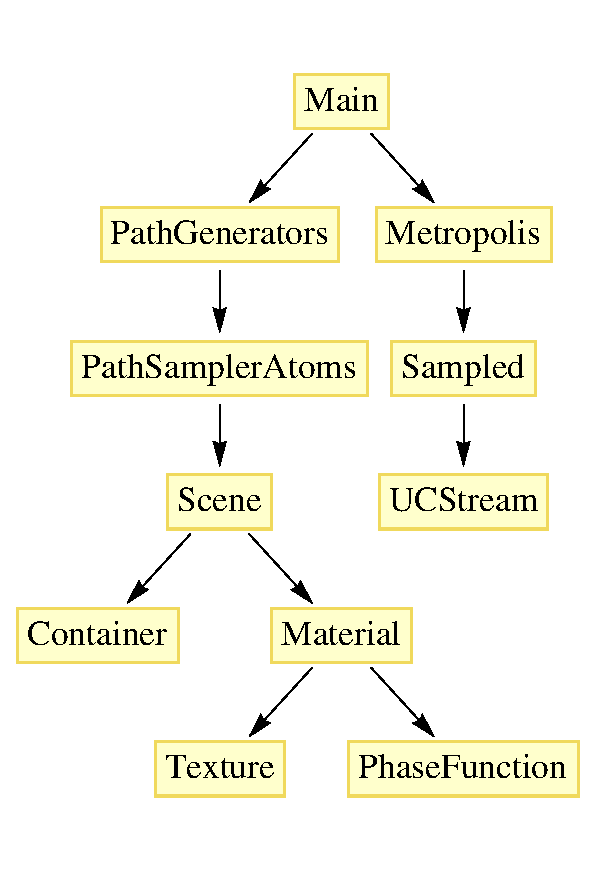
\includegraphics[height=0.3\textheight]{moduleoverview.eps}
				\caption{Illustration der Modulhierarchie in \texttt{PIRaTE}.}
				\label{fig:moduleoverview}
		\end{figure}
		%\begin{wrapfigure}{r}{0.6\textwidth}
		%	\centering
		%	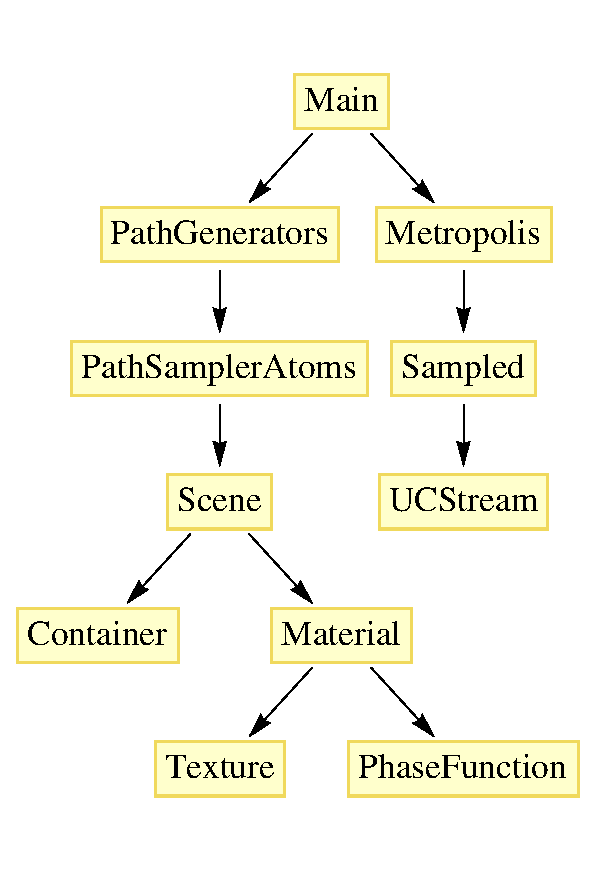
\includegraphics[height=0.2\textheight]{moduleoverview.eps}
		%	\caption{Modulhierarchie in \texttt{PIRaTE}.}
		%	\label{fig:moduleoverview}
		%\end{wrapfigure}
	Das Modul \textbf{Scene} erlaubt die Beschreibung eines konkreten Strahlungstransportproblems (im Folgenden Szene genannt) und stellt eine Schnittstelle zur Abfrage von Informationen innerhalb der Szene bereit. Eine Szene besteht dabei aus einer Liste von Containern, die mit einem oder mehreren Materialien gefüllt sein können. Ein Container repräsentiert ein (meist abgeschlossenes) Raumgebiet wie z.B. eine Kugel oder ein Quader. Für jeden Container müssen dabei Funktionen implementiert sein, die angeben, ob ein Raumpunkt innerhalb des Containers liegt, ob und wo ein Strahl den Container schneidet, sowie eine Abbildung aus dem dreidimensionalen Einheitswürfel auf Raumpunkte innerhalb des Containers. Ein Material besteht aus Skalarfeldern für Absorptionquerschnitt, Streuquerschnitt, Emissivität und Sensitivität sowie getrennten Phasenfunktionen für Emission, Streuung und Sensation. Skalarfelder sind im Modul \textbf{Texture} definiert und erlauben sowohl homogene Skalarfelder mit einem konstanten Wert als auch inhomogene Skalarfelder, die durch eine beliebige Funktion aus $\mathbb{R}^3\to\mathbb{R}$ jedem Raumpunkt einen Wert zuordnen. Phasenfunktionen sind im Modul \textbf{Phasefunction} definiert. Wie bei Containern muss zur Definition einer Phasenfunktion eine Abbildung aus $[0,1]^2\to\mathcal{S}^2$ angegeben werden, die zwei Zahlen aus dem Einheitsintervall auf eine Raumrichtung abbilden. Nach der Definition einer Szene durch Kombination von Materialien und Containern stellt \textbf{Scene} eine Schnittstelle bereit, mit dem sich punktuelle Eigenschaften, wie der Absorptionsquerschnitt, die Albedo, Emissivität oder eine Liste aller Streuphasenfunktionen an einem Ort abfragen lassen. Ausserdem lassen sich optische Tiefen abfragen, entweder zwischen zwei Punkten oder von einem Punkt aus in eine bestimmte Raumrichtung, bis ein festgelegtes Distanz- oder optisches Tiefenziel erreicht ist. Zur Berechnung der optischen Tiefen wird entlang des Strahls eine Liste disjunkter Intervalle gefüllt mit homogenem Material berechnet. Ist eines der beteiligten Materialien inhomogen, wird es stückweise durch homogene Intervalle ersetzt, deren Werte durch Mittelung der inhomogenen Funktion mittels eines Gauss--Legendre--Verfahrens bestimmt werden.
	
	Auf diese Schnittstelle baut das Modul \textbf{PathSamplerAtoms} auf. Es stellt Methoden zum Samplen von Punkten, Richtungen und Distanzen für Emission, Streuung und Sensation bereit (s. Tab.~\ref{tab:pathsampleratoms}).
	\begin{table}[htdp]
		\caption{Alle neun vom Modul \textbf{PathSamplerAtoms} bereitgestellten Methoden. Der Pfeil beschreibt aus welchen Eingangswerten welches Ergebnis gezogen wird.}
		\begin{center}
		\begin{tabular}{|c|c|c|}
			\hline
			Punkt--Sampler & Richtungs--Sampler & Distanz--Sampler \\
			\hline
			Szene & (Szene,einfallender Strahl) & (Szene,ausgehender Strahl) \\
			$\downarrow$ & $\downarrow$ & $\downarrow$ \\
			Punkt & ausgehende Richtung & Distanz \\
			\hline\hline
			SensationPointSampler & SensationDirectionSampler & SensorDistanceSampler \\
			ScatteringPointSampler & ScatteringDirectionSampler & ScattererDistanceSampler \\
			EmissionPointSampler & EmissionDirectionSampler & EmitterDistanceSampeler \\
			\hline
		\end{tabular}
		\end{center}
		\label{tab:pathsampleratoms}
	\end{table}%
	So erlaubt z.B. der {\em SensationPointSampler} aus einer Szene einen zufälligen Raumpunkt zu ziehen, der innerhalb einer der Container liegt, die ein sensitives Material beinhalten. Der {\em ScatteringDistanceSampler} erlaubt, aus einer Szene und einem einfallenden Strahl (d.h. einem Streuort und einer Richtung aus der das Photon kommt) eine ausgehende Richtung zu samplen, in die das Photon gestreut wird. Mithilfe des {\em EmitterDistanceSampler} lässt sich aus einer Szene einem Ort und einer ausgehenden Richtung eine zufällige Distanz bis zum nächsten Emissionspunkt ziehen. Dabei werden beim Ziehen aus einem Punkt--Sampler die von den Containern bereitgestellten, obengenannten Abbildungen auf Punkte in ihrem Volumen benutzt. Ebenso greifen die Richtungs--Sampler auf die von den Phasenfunktionen am spezifizierten Ort bereitgestellten Abbildungen auf eine Richtung zurück. Der {\em ScatteringDirectionSampler} berücksichtigt ausserdem die angegebene einfallende Richtung, {\em EmissionDirectionSampler} sowie {\em SensationDirectionSampler} können diese ignorieren, da Emission und Sensation terminale Prozesse sind, so dass nur eine Richtung in die jeweiligen Phasenfunktionen eingeht. {\em EmitterDistanceSampler} und {\em SensorDistanceSampler} implementieren den in Abschnitt \ref{subsubsec:distancesampler}  vorgestellten Distanzsampler $P_1$, {\em ScattererDistanceSampler} implementiert den Distanzsampler $P_3$. In der aktuellen Version von \pirate wird nicht von all diesen Samplern Gebrauch gemacht. Die Implementation all dieser Sampler, erlaubt aber eine hohe Flexibilität und eine leichte Implementation zukünftiger Pfadgenerierungsverfahren.
	
	Mithilfe der in \textbf{PathSamplerAtoms} bereitgestellten Grundbausteine wird im Modul \textbf{PathGenerators} das Verfahren zum Generieren kompletter Pfade aus Abschnitt \ref{subsec:sensor_based_raycasting} implementiert. Die Wahrscheinlichkeit $p_\text{grow}$, einen zu\-sätz\-lich\-en Streupunkt zu generieren, ist dabei ein freier Parameter der für jede Simulation neu angegeben werden kann.
	
	Im Modul \textbf{Sampled} wird eine Schnittstelle für samplebare Objekte jeder Art definiert. Dies beinhaltet eine Funktion, die aus einem Strom aus Zufallszahlen ein Sample generieren kann, sowie Funktionen um die entsprechende Wahrscheinlichkeitsdichte, sowie einen eventuellen Beitrag des Samples zu berechnen. Dies wird im Programm an allen Stellen benutzt, wo zufällige Stichproben generiert werden, z.B. beim Samplen eines Punktes aus einem Container, dem Samplen einer Raumrichtung aus einer Phasenfunktion oder dem Samplen eines kompletten Pfades aus einer Pfadgenerierungsmethode. Im Fall eines Pfades ${\overline x}$, wird so neben dem Pfad als Sample auch das Verhältnis aus Messbeitragsfunktion $f({\overline x})$ und Generierungswahrscheinlichkeit $p({\overline x})$ berechnet. Durch die Möglichkeit, direkt das Verhältnis beider Ausdrücke zu berechnen, wird die Pfadgenerierung wesentlich effizienter, da sich viele gemeinsame Faktoren herauskürzen. Durch diese feste Schnittstelle ist es möglich die Kombination einfacher Samplingmethoden zu komplexeren wieder als eine Funktion zu reduzieren, die aus einer unendlich langen Liste von Zufallszahlen Samples generieren kann.
	
	Das \textbf{Metropolis}--Modul implementiert den in Abschnitt \ref{sec:robustmetropolis} vorgestellten abgewandelten Metropolis--Hastings--Algorithmus. Im Gegensatz zum klassischen MH--Algorithmus gewichten wir generierte Pfade aber nicht voll oder garnicht (bei Ablehnung des Samples), sondern gewichten jedes Sample mit seiner Akzeptanzwahrscheinlichkeit. Dieses Vorgehen hat den selben Erwartungswert, nutzt aber auch die abgelehnten Samples, was zu einem effizienteren Verfahren führt. Hierdurch können insbesondere Pfade zur Konvergenz der Messung beitragen, die nur eine sehr geringe Wahrscheinlichkeit haben gesampelt zu werden. In Pseudocode:
	
	\begin{algorithmic}
		\REPEAT[finde beitragenden Pfad]
		\STATE $u \leftarrow$ Anfangszustand
		\STATE $x \leftarrow S(u)$
		\UNTIL{$f(x_1)>0$}
		\STATE $w = 1$ \COMMENT{Gewicht des aktuellen Samples}
		\FOR{$i=1$ to $N$}
			\STATE $r\leftarrow$ Zufallszahl aus $[0,1]$
			\IF[Mutation schlägt frisches Sample vor]{$r < p_\text{fresh}$}
				\STATE $T \leftarrow T_\text{fresh}$
			\ELSE[Mutation schlägt leicht abgewandeltes Sample vor]
				\STATE $T \leftarrow T_\text{perturb}$
			\ENDIF
			\STATE $u'\leftarrow$ ziehe Wert gemäß $T(u'|u)$
			\STATE $x' \leftarrow S(u')$
			\STATE $a(u'|u) \leftarrow \text{min}\left(1,\frac{f(x')}{f(x_i)}\right)$
			\STATE $r\leftarrow$ Zufallszahl aus $[0,1]$
			\IF{$r < a(u'|u)$}
				\STATE $x_i \leftarrow x$
			  \STATE $w_i \leftarrow w+(1-a(u'|u))$
				\STATE $u \leftarrow u'$
			  \STATE $x \leftarrow x'$
			  \STATE $w \leftarrow a(u'|u)$
			\ELSE
				\STATE $x_i \leftarrow x'$
				\STATE $w_i \leftarrow a(u'|u)$
				\STATE $w \leftarrow (1-a(u'|u))$
			\ENDIF
	  \ENDFOR
	  \STATE\COMMENT{gebe Liste gewichteter Samples zurück}
	  \RETURN{$(w,x)$}
	\end{algorithmic}
	
	Im Modul \textbf{UCStream} (={\em UnitCoordinatesStream}) werden Funktionen zum Generieren dieser unendlich langen Listen aus Zufallszahlen definiert. Darüber hinaus werden auch Funktionen zur Variation eines solchen Zufallszahlenstroms durch kleine zufällige Störungen mit einem anderen Zufallszahlenstrom definiert.
	
	Das Modul \textbf{Main} ruft den Metropolis--Algorithmus mit dem Pfadgenerierungsverfahren aus \textbf{PathGenerators} auf und extrahiert aus der Liste gewichteter Pfade die Verteilung der Pfade über den virtellen CCD--Sensor und gibt das durch Binning entstehende Bild in eine Datei aus.
	
	Der Quellcode von \pirate ist unter
	
	\url{http://github.com/theidecke/PIRaTE}
	
	öffentlich zugänglich.
	
	
	
	
	
		\chapter{Testf"alle und Resultate}
	In diesem Abschnitt sollen die Ergebnisse und die Effizienz des in Abschnitt \ref{cha:program_description} vorgestellten Programmes anhand von zwei unterschiedlichen Testf"allen analysiert werden. Als Referenz dient dabei das Programm \texttt{MC3D} \citep{Wolf:2003p12974}, sowohl f"ur die berechneten Bilder als auch f"ur die Geschwindigkeit der Berechnung. F"ur den ersten Testfall wurde zur Berechnung einer Referenzl"osung zus"atzlich zum einen ein geschlossener Ausdruck f"ur die L"osung hergeleitet und zum anderen ein einfaches Monte--Carlo--Verfahren erdacht, das sehr schnell konvergiert.
	
	\section{Homogene streuende Kugel}
	Um die Korrektheit der vom Monte--Carlo--Code produzierten L"osung zu verifizieren ist es von erheblichem Nutzen eine unabh"angig gewonnene, vielleicht sogar analytisch hergeleitete, L"osung eines konstruierten Testproblems berechnen zu k"onnen. Das Problem sollte dabei nicht so trivial sein, dass komplexe Effekte wie Mehrfachstreuung keinen Einflu"s auf das Ergebnis haben. Gleichzeitig sollte es aber nicht so komplex sein, dass keine elegante, leicht berechenbare L"osung gefunden werden kann.
	Mit dieser Motivation konstruieren wir folgendes Testproblem:
		
	Gegeben sei eine Kugel mit Radius $R$, die mit homogenem, isotrop streuendem Material mit Volumenstreuquerschnitt $\sigma=1$ gef"ullt ist, sowie eine punktf"ormige Lichtquelle im Zentrum der Kugel. Zu berechnen ist nun die radiale Abh"angigkeit der Intensit"at, die eine ausserhalb der Kugel platzierte orthographische Kamera, die zum Zentrum der Kugel ausgerichtet ist, misst. Die feste Wahl von $\sigma$ und Variation des Kugelradius $R$ dient ausschliesslich der einfacheren Berechnung, da die Wegstrecken dadurch automatisch in freien optischen  Wegl"angen $\lambda=1/\sigma$ vorliegen. Das Problem ist gleichwertig zu jeder anderen Kombination aus Radius und Volumenstreuquerschnitt f"ur welche sich die gleiche optische Tiefe $\tau_\text{center}=\sigma R=R/\lambda$ vom Zentrum bis zum Rand der Kugel ergibt.
	
	\begin{figure}
			\centering
			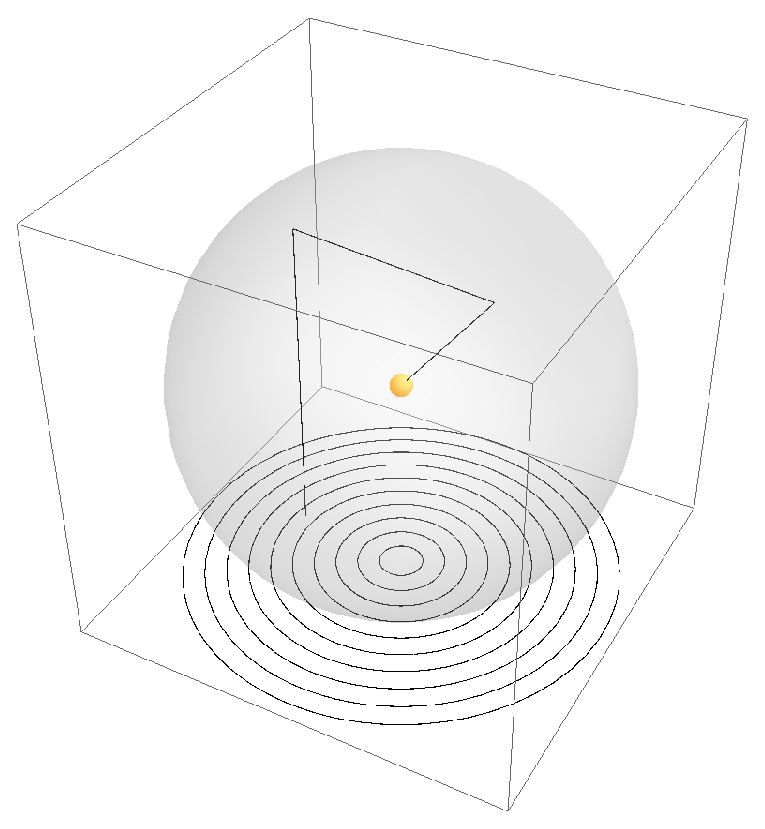
\includegraphics[height=0.45\textheight]{testproblem_illustration.eps}
			\caption{Illustration des Testproblems. Gezeigt ist ein Photonenpfad der zweimal gestreut wird und in einem ringf"ormigen Bin der orthographischen Kamera auftrifft}
			\label{fig:testproblem_sketch}
	\end{figure}

	
	\subsection{analytische L"osung}\label{subsec:homsphere_analytic_solution}
	\subsubsection{Green'sche Funktion f"ur den Photonentransport zwischen Kugelschalen}
	Um die korrekte radiale Intensit"atsverteilung zu berechnen, bestimmen wir zun"achst in Form der Green'schen Funktion $g$, wie sich die Photonen radial nach einem Streuvorgang ausgebreitet haben.
	Genauer gibt $g$ an, wie gro"s der Anteil der Photonen, die auf einer Kugelschale mit Radius $r_0$ starten, beim Radius $r_1$ w"ahrend des n"achsten Streuvorganges ist (siehe Abb. \ref{fig:radial_greens_function_pdfcdf}):
	\begin{align*}
		g(r_0,r_1) =& 2 \pi \int_0^\pi r_1^2 \sin(\theta) \frac{\exp\left(-\sqrt{r_0^2-2 r_0 r_1 \cos(\theta)+r_1^2}\right)}{4 \pi (r_0^2-2 r_0 r_1 \cos(\theta)+r_1^2)} \text{d}\theta \\
		=& \frac{1}{2}\frac{r_1}{r_0} \int_{|r_0-r_1|}^{r_0+r_1} \frac{e^{-t}}{t} dt \\
		=& \frac{1}{2}\frac{r_1}{r_0}\left[\text{Ei}(-(r_0+r_1)) - \text{Ei}(-|r_0-r_1|)\right]
	\end{align*}
	
	\begin{figure}
		\centering
		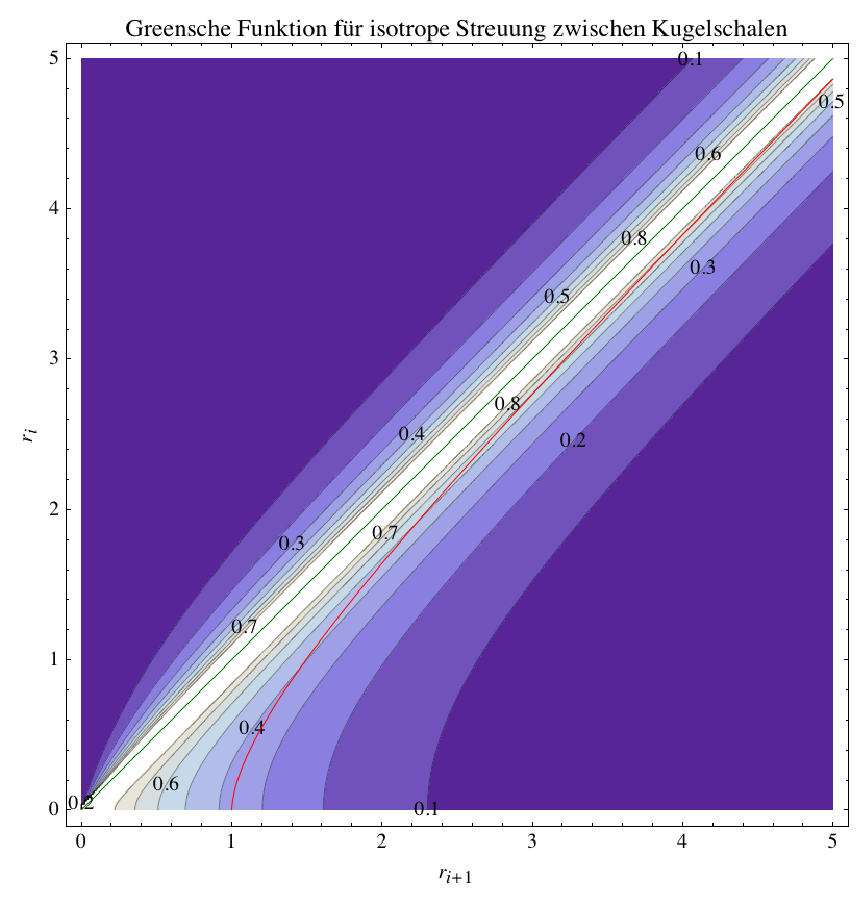
\includegraphics[width=0.48\textwidth]{radial_greens_function_pdf.eps}
		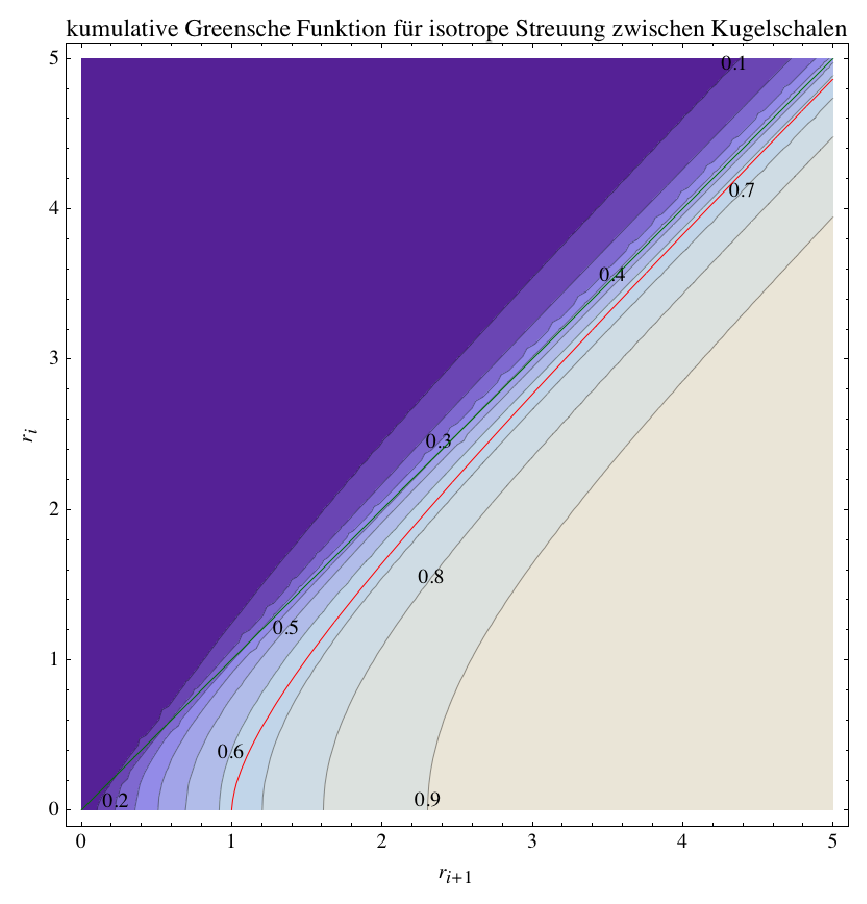
\includegraphics[width=0.48\textwidth]{radial_greens_function_cdf.eps}
		\caption{Green'sche Funktion der radialen Teilchenverteilung die von Radius $r_i$ kommen und beim Radius $r_{i+1}$ streuen als PDF und CDF. Der mittlere Radius ist in rot eingezeichnet.}
		\label{fig:radial_greens_function_pdfcdf}
	\end{figure}
	\begin{figure}
		\centering
		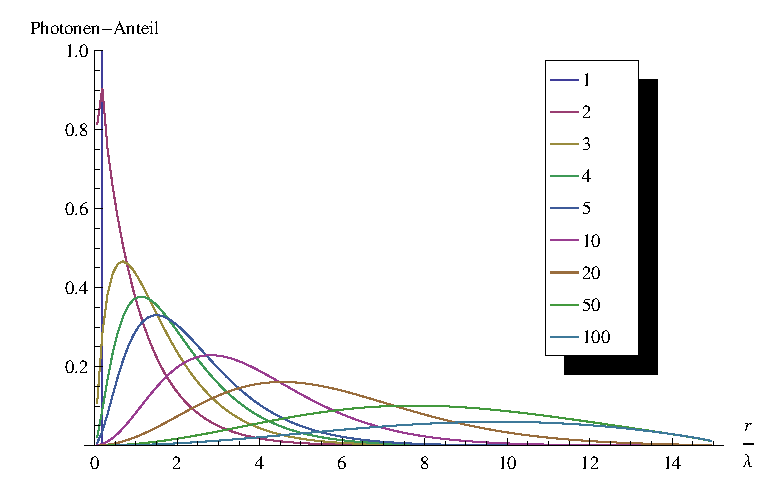
\includegraphics[width=0.9\textwidth]{gnlist_plot.eps}
		\caption{radiale Photonenverteilung nach n Streuvorg"angen. Die freie optische Wegl"ange ist dabei mit $\lambda=1/\sigma$ bezeichnet.}
		\label{fig:gnlist}
	\end{figure}
	Als n"achstes diskretisieren wir die Green'sche Funktion, indem wir ein gleichm"assiges Gitter in $r_0$ und $r_1$ "uber $g$ legen, das sich bis zum Radius der Kugel $R$ erstreckt, und innerhalb jeder Gitterzelle $g$ in $r_0$--Richtung mitteln und in $r_1$--Richtung aufintegrieren und anschliessend die Ergebnisse in einer Matrix $\mathbf{g}$ speichern. Wenn wir nun einen Startvektor, der nur in der innersten Zelle von Null verschieden ist, $n$--mal mit $\mathbf{g}$ multiplizieren, bekommen wir die diskretisierte Photonenverteilung innerhalb der Kugelschalen beim $n$--ten Streuvorgang (siehe Abb. \ref{fig:gnlist}). Um die Emissivit"at $\varepsilon(r)$ jeder Kugelschale auszurechnen, summieren wir die Photonenverteilungen vom 1--ten bis zum $n$--ten Streuvorgang auf und teilen das Ergebnis in jeder Kugelschale durch ihr jeweiliges Volumen und den bestrahlten Raumwinkel $4\pi$. Die Intensit"aten k"onnen nun numerisch gem"a"s
	\begin{equation}
		I(r) = \int_{z=-h}^h \varepsilon\left(\sqrt{r^2+z^2}\right) e^{-(z+h)}\text{d}z\,,\quad h=\sqrt{R^2-r^2}
		\label{eq:testprob_intensity_calculation}
	\end{equation}
	berechnet werden.
	
	%\begin{figure}
	%	\centering
	%	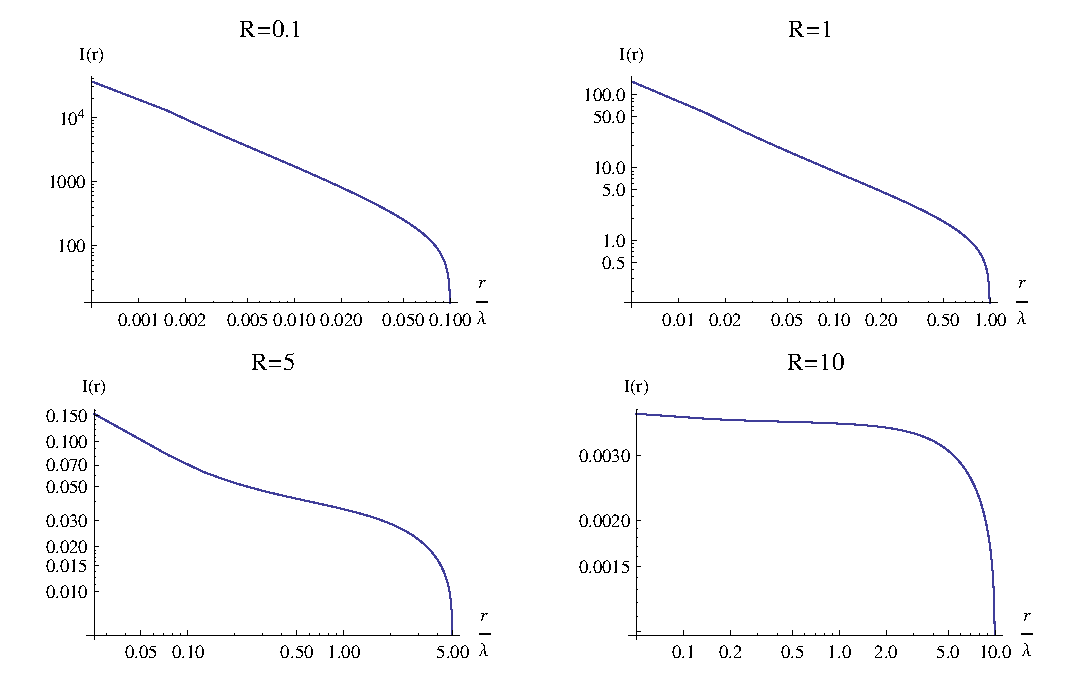
\includegraphics[width=1.0\textwidth]{analytical_tau_comparison.eps}
	%	\caption{radiales Intensit"atsprofil f"ur verschiedene Kugelradien und damit verschiedene optische Tiefen. $\lambda=1/\sigma$ bezeichnet die freie optische Wegl"ange.}
	%	\label{fig:analytical_tau_comparison}
	%\end{figure}
	
	%Das Ergebnis ist f"ur vier Kugelradien beispielhaft in Abb. \ref{fig:analytical_tau_comparison} dargestellt.
	
	\pagebreak
	\subsection{schnelle Monte--Carlo--L"osung}
	Eine andere Methode, schnell die radiale Intensit"atsverteilung zu bestimmen, ist durch folgendes Monte--Carlo--Schema gegeben:
	\begin{algorithmic}
		\STATE $M\leftarrow$ Anzahl Ringe
		\STATE $N\leftarrow$ Anzahl Photonen
		\STATE $R\leftarrow$ Kugelradius
		\FOR{$i=1$ to $N$}
			\STATE $\location{r}\leftarrow (0,0,0)^\text{T}$
			\REPEAT
				\STATE\COMMENT{w"ahle zuf"allige Richtung $\omega$}
				\STATE $z\leftarrow$ ziehe gleichf"ormig aus $[-1,1]$
				\STATE $\phi\leftarrow$ ziehe gleichf"ormig aus $[0,2\pi]$
				\STATE $s\leftarrow\sqrt{1-z^2}$
				\STATE $\omega\leftarrow (s\;\text{cos}(\phi),s\;\text{sin}(\phi),z)^\text{T}$
				\STATE\COMMENT{w"ahle exponentiell verteilte Entfernung $t$}
				\STATE $u\leftarrow$ ziehe gleichf"ormig aus $[0,1]$
				\STATE $t\leftarrow -\text{ln}(1-u)$
				\STATE $\location{r}_\text{old}\leftarrow\location{r}$
				\STATE $\location{r}\leftarrow\location{r}_\text{old}+\omega t$
			\UNTIL{$|\location{r}|\geq R$}
			\STATE\COMMENT{bestimme Sto"sparameter $b$}
			\STATE $\location{d}\leftarrow\location{r}-\location{r}_\text{old}$
			\STATE $b\leftarrow\sqrt{\langle\location{r},\location{r}\rangle-\frac{\langle\location{r},\location{d}\rangle}{\langle\location{d},\location{d}\rangle}}$
			\STATE $j\leftarrow\lfloor M\frac{b}{R}\rfloor$
			\STATE $C[j]=C[j]+1$
		\ENDFOR
		\FOR[normiere Bincounts mit Ringfl"achen]{$j=0$ to $M-1$}
			\STATE $C[j]=C[j]/(\pi R^2(2j+1)/M^2)$
		\ENDFOR
		\RETURN $C[\cdots]$
	\end{algorithmic}
	Dabei starten wir mit einem Photon im Ursprung und berechnen dann von der aktuellen Position solange die Position des n"achsten Streuereignisses, bis dieses ausserhalb der Kugel liegt. Damit kennen wir den letzten Streupunkt und die Richtung in die das Photon das Streuvolumen verl"asst. Da wir nur an der radialen Intensit"atsverteilung interessiert sind k"onnen wir die Symmetrie des Problems ausnutzen indem wir die Kamera immer so hindrehen, dass das entfliehende Photon senkrecht auf den (gedachten) Sensor auftrifft. Das bedeutet, dass nicht die genaue Entweichrichtung sondern nur der Sto"sparameter entscheidend ist. Mit diesem Trick k"onnen wir jedes entweichende Photon z"ahlen, sodass dieses Verfahren sehr schnell konvergiert.
	
	
	\subsection{Resultate}
	TODO: Geschwindigkeits--Vergleich mit MC3D
	
	Um die korrekte Berechnung des Strahlungstransports "uberpr"ufen zu k"onnen, simulieren wir das vorgestellte Problem der homogen streuenden Kugel f"ur drei verschiedene Radien (und damit optische Tiefen) jeweils mit der in Abschnitt~\ref{subsec:homsphere_analytic_solution} vorgestellten Methode, die wir als Referenzl"osung benutzen. Dieselben Konfigurationen berechnen wir ausserdem mit \texttt{MC3D} und \texttt{PIRaTE}. Von \texttt{MC3D} lassen wir hierf"ur $3.6\cdot10^8$ Photonen generieren und von 72 virtuellen Kameras, die auf einem Kreis auf das Zentrum blickend im Abstand von 5 Grad verteilt sind, beobachten. Jede Kamera ist dabei in einem Kegel mit "Offnungswinkel von $\alpha=5^\circ$ f"ur eintreffende Photonen empfindlich\footnote{In Abb.~\ref{fig:alphacomparison} ist der Effekt unterschiedlicher Kamera"offnungswinkel $\alpha$ bei gleicher Photonenanzahl gezeigt.}. \texttt{PIRaTE} benutzt eine einzige Kamera deren Empfindlichkeitskegel einen "Offnungswinkel von $30'$ besitzt.
	
		\begin{figure}
			\centering
			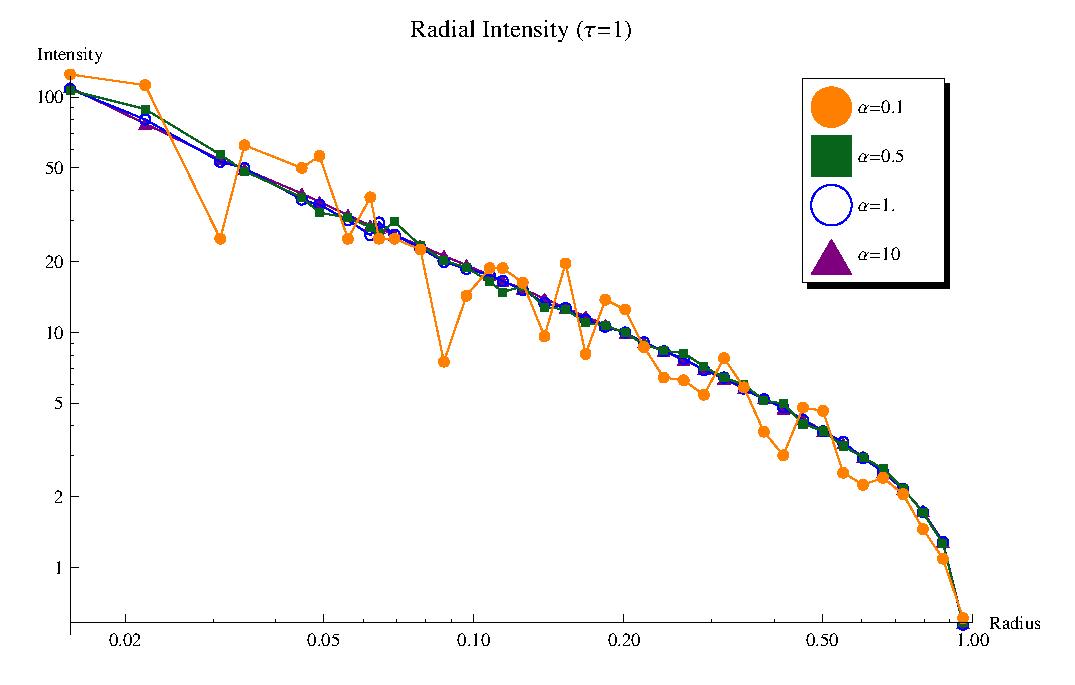
\includegraphics[width=0.8\textwidth]{mc3dalphasplot.eps}
			\caption{Radiale Intensit"atsprofile auf der Grundlage von \texttt{MC3D}--Simulationen --- Bei gleicher Photonenzahl aber sinkendem Kamera--"Offnungswinkel $\alpha$ steigt der statistische Fehler aufgrund der geringeren Zahl beachteter Photonen.}
			\label{fig:alphacomparison}
		\end{figure}
	
	Die drei gew"ahlten optischen Tiefen $\tau\in\{0.01,1,10\}$ decken dabei den optisch d"unnen, mittleren und dicken Fall ab.	In Abb.~\ref{fig:methodcomparisongraphics} sind mit der analytischen Methode, \texttt{MC3D} und \texttt{PIRaTE} gewonnene radiale Intensit"atsprofile abgebildet.
	Im dargestellten Bereich stimmen die Ergebnisse beider Programme im Rahmen des statistischen Fehlers gut mit der analytischen L"osung "uberein. Dabei ist zu bedenken, dass bei kleineren Radien "uber weniger Pixel der zugrundeliegenden Bilder gemittelt wird und somit der statistische Fehler dort naturgem"a"s gr"o"ser ausf"allt.
		\begin{figure}
			\centering
			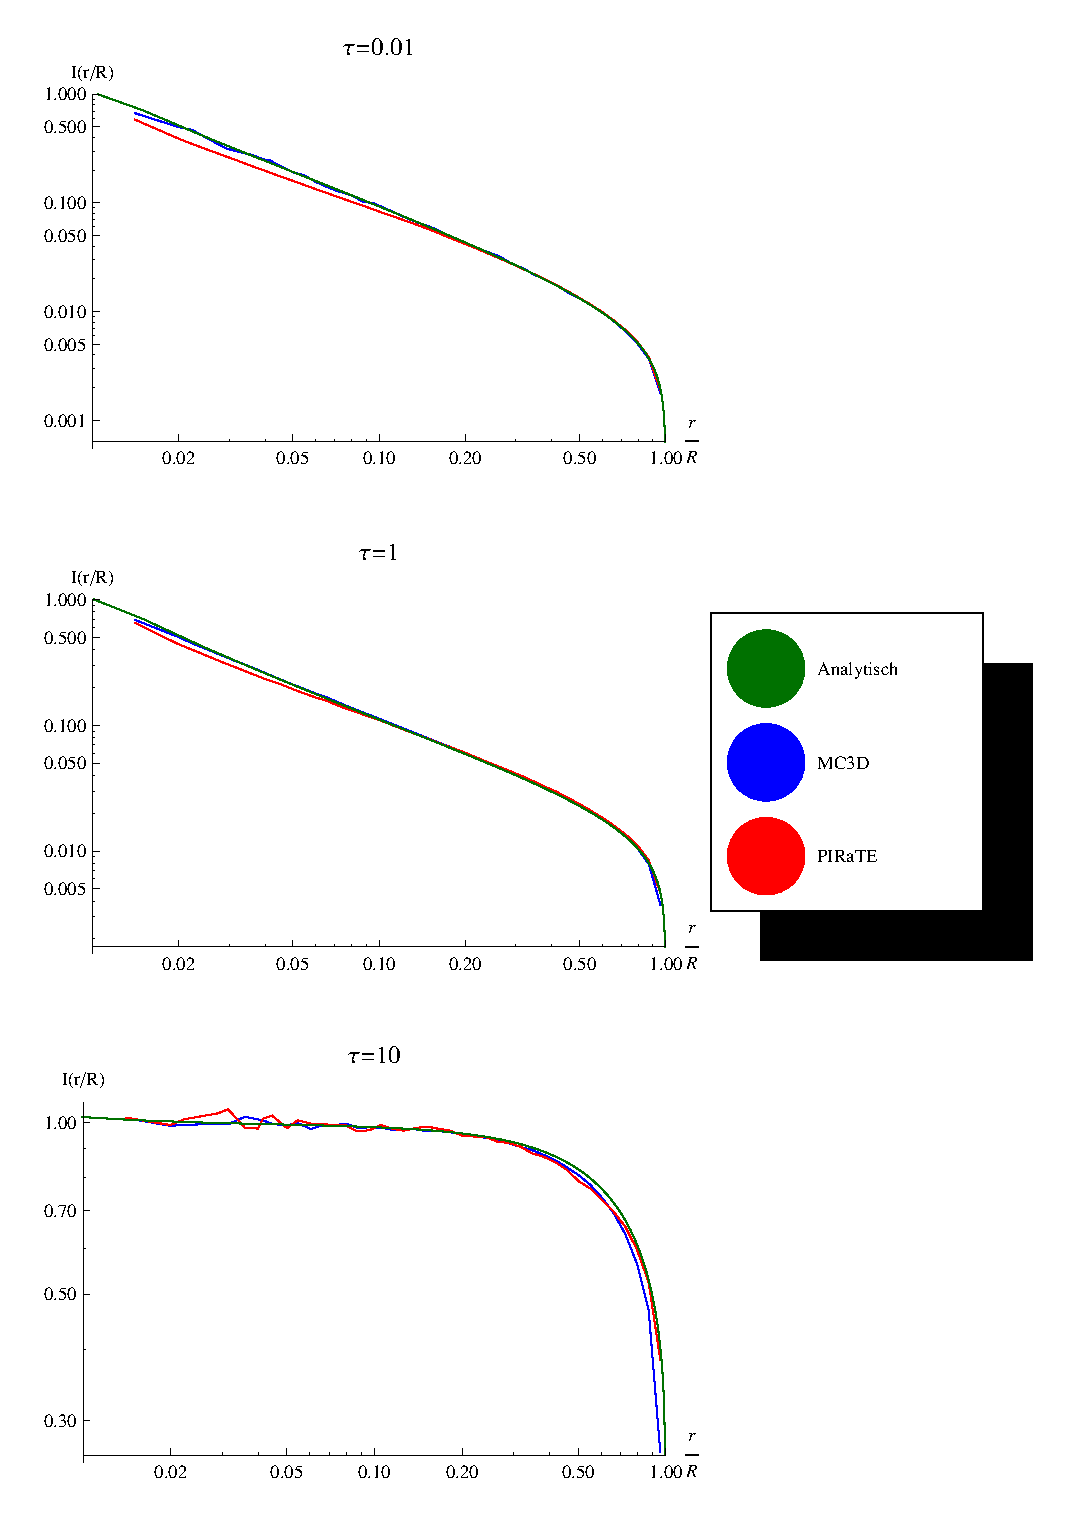
\includegraphics[height=1.0\textheight]{methodcomparisongraphics.eps}
			\caption{Vergleich zwischen der analytischen L"osung, \texttt{MC3D} und \texttt{PIRaTE} bei verschiedenen optischen Tiefen. \texttt{MC3D} hat f"ur alle drei F"alle $3.6\cdot10^8$ Photonen, \texttt{PIRaTE} jeweils $4.88\cdot10^7,4.88\cdot10^7,2.088\cdot10^8$ Photonenpfade generiert.}
			\label{fig:methodcomparisongraphics}
		\end{figure}
	
	Bei Betrachtung von horizontalen Schnitten durch die Streubilder (siehe Abb.~\ref{fig:sphere_image_cuts}) f"allt auf, das \texttt{PIRaTE} den Anteil des direkt von der Punktlichtquelle kommenden Lichtes falsch sch"atzt. Dies liegt vermutlich an den Sensorparametern ("Offnungswinkel), da im Unterschied zu \texttt{MC3D} in \texttt{PIRaTE} keine punktf"ormigen sondern nur ausgedehnte Lichtquellen existieren, die bei kleinen Ausma"sen mit der jetzigen Pfadgenerierungsmethode schwer zu samplen sein k"onnen. Zur end"ultigen Kl"arung bedarf es aber einer genaueren Fehleranalyse.
	
		\begin{figure}
			\centering
			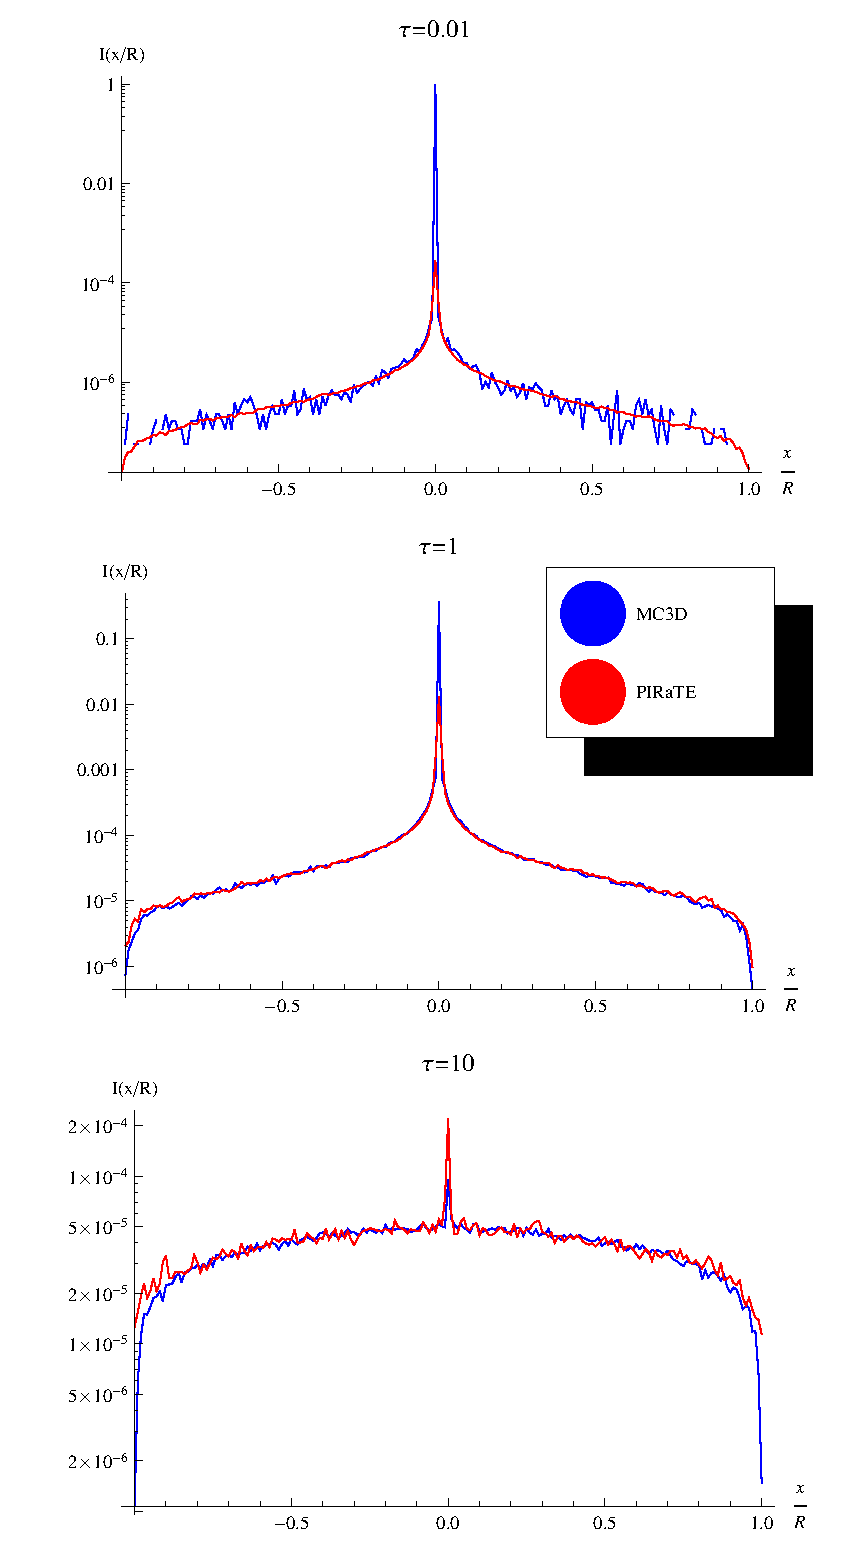
\includegraphics[height=1.0\textheight]{sphere_image_cuts.eps}
			\caption{Horizontale Schnitte durch die Streubilder f"ur die drei optischen Tiefen bei hoher Anzahl an Photonen bzw. Pfade.}
			\label{fig:sphere_image_cuts}
		\end{figure}
	
	Um nicht komplett auf einen Vergleich der Konvergenzraten beider Programme verzichten zu m"ussen, verwenden wir zur Berechnung der Abweichung vom Referenzbild maskierte Bilder, bei denen die Lichtquelle in der Mitte des Bildes ausgeblendet ist.	 Die Referenzbilder (siehe Abb.~\ref{fig:sphere_reference_images}) werden dabei aus den, aus allen 72 Kameraebenen akkumulierten, von \texttt{MC3D} erzeugten Streubildern generiert. Zus"atzlich mitteln wir innerhalb der Bildes "uber alle Pixelgruppen mit exakt gleichem Abstand vom Zentrum (siehe Abb.~\ref{fig:polaraveragingsymmetry}). Dies f"uhrt im Durchschnitt zu einer Mittelung "uber 11 Pixel wodurch das Rauschen ungef"ahr gedrittelt wird, was insbesondere bei dem Bild der optisch d"unnen Kugel, welches das st"arkste Rauschen besitzt, hilfreich ist.
	
		\begin{figure}
			\centering
			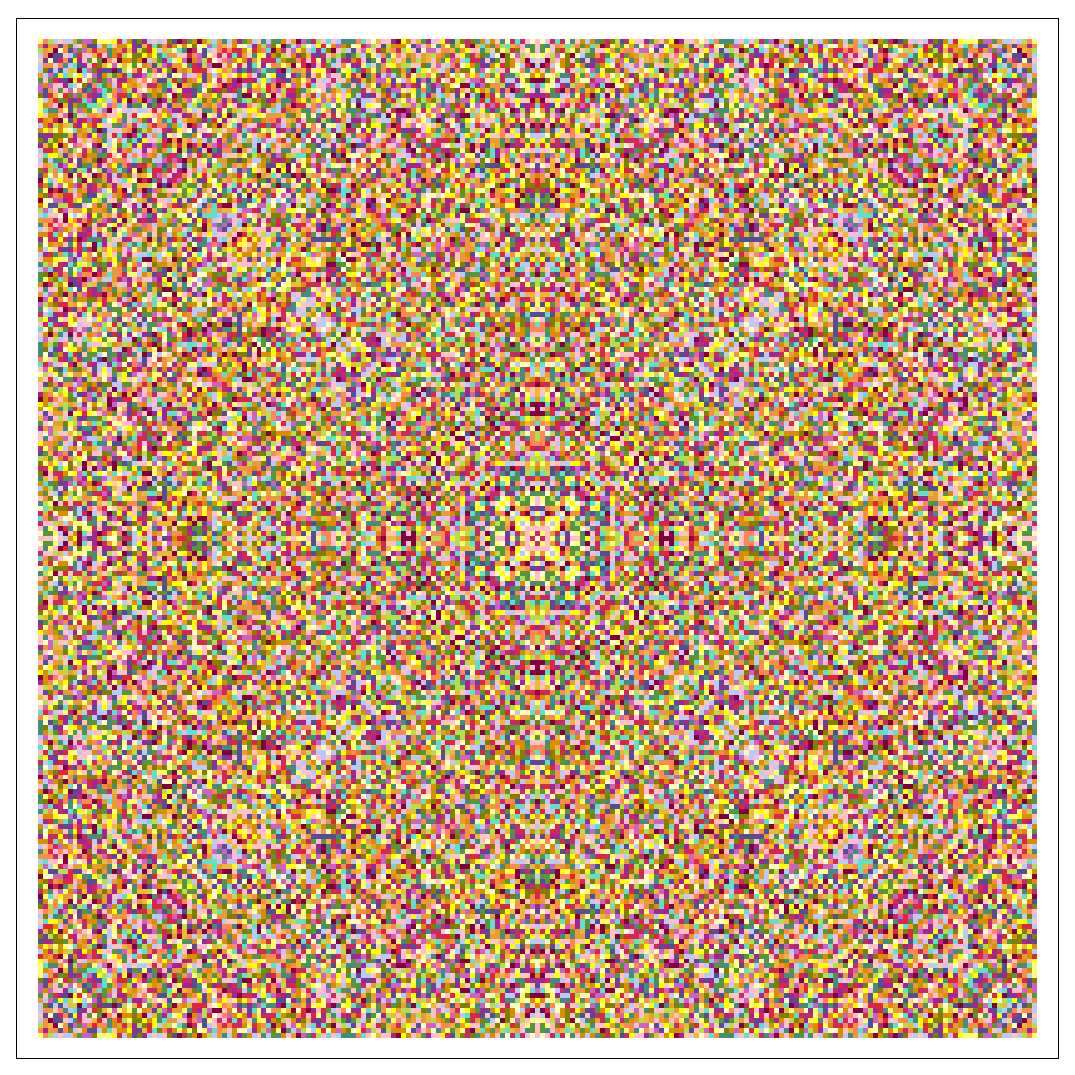
\includegraphics[width=0.5\textwidth]{polaraveragingsymmetry.eps}
			\caption{Darstellung der Symmetrien, die bei der polaren Mittelung genutzt werden. Pixel mit exakt gleichem Abstand zum Zentrum sind gleich gef"arbt. Im Schnitt wird "uber 11 Pixel gemittelt.}
			\label{fig:polaraveragingsymmetry}
		\end{figure}
		
		\begin{figure}
			\centering
			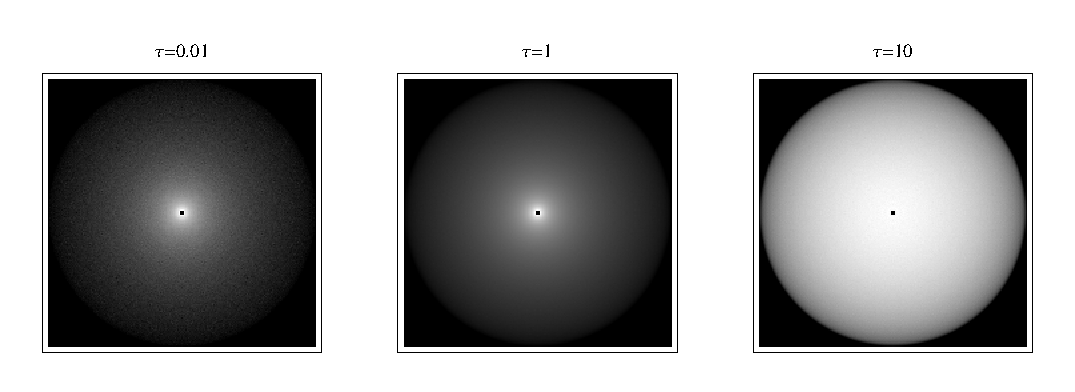
\includegraphics[width=1.0\textwidth]{spherereferenceimages.eps}
			\caption{Referenzbilder zur Bestimmung der Abweichungen}
			\label{fig:sphere_reference_images}
		\end{figure}
	
		\begin{figure}
			\centering
			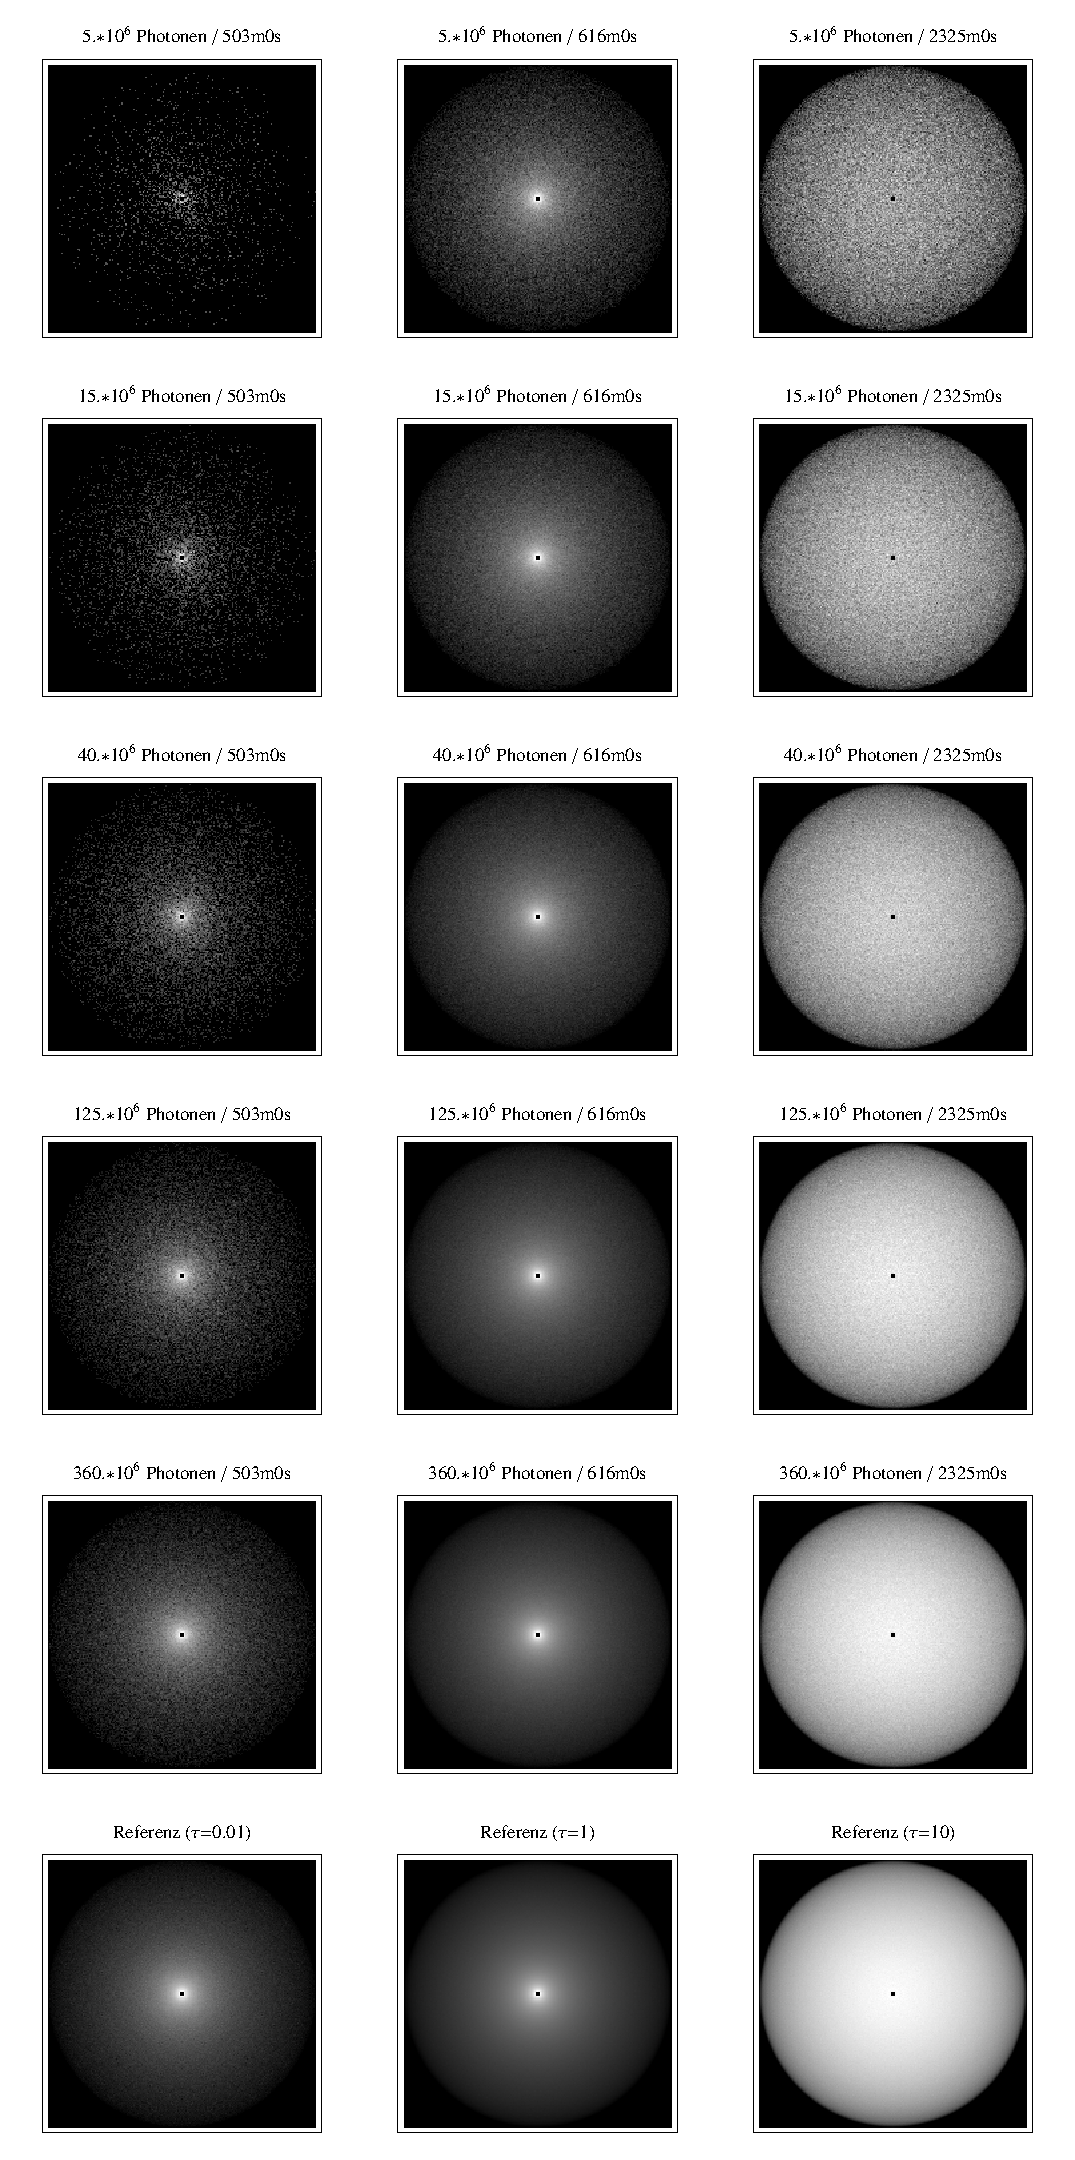
\includegraphics[height=1.0\textheight]{mc3dsphereimageoverview.eps}
			\caption{"Ubersicht "uber die Qualit"at der Bilder bei Akkumulation unterschiedlich vieler Kameraebenen der \texttt{MC3D}--Simulationen und der Simulationszeiten.}
			\label{fig:mc3d_sphere_imageoverview}
		\end{figure}
		\begin{figure}
			\centering
			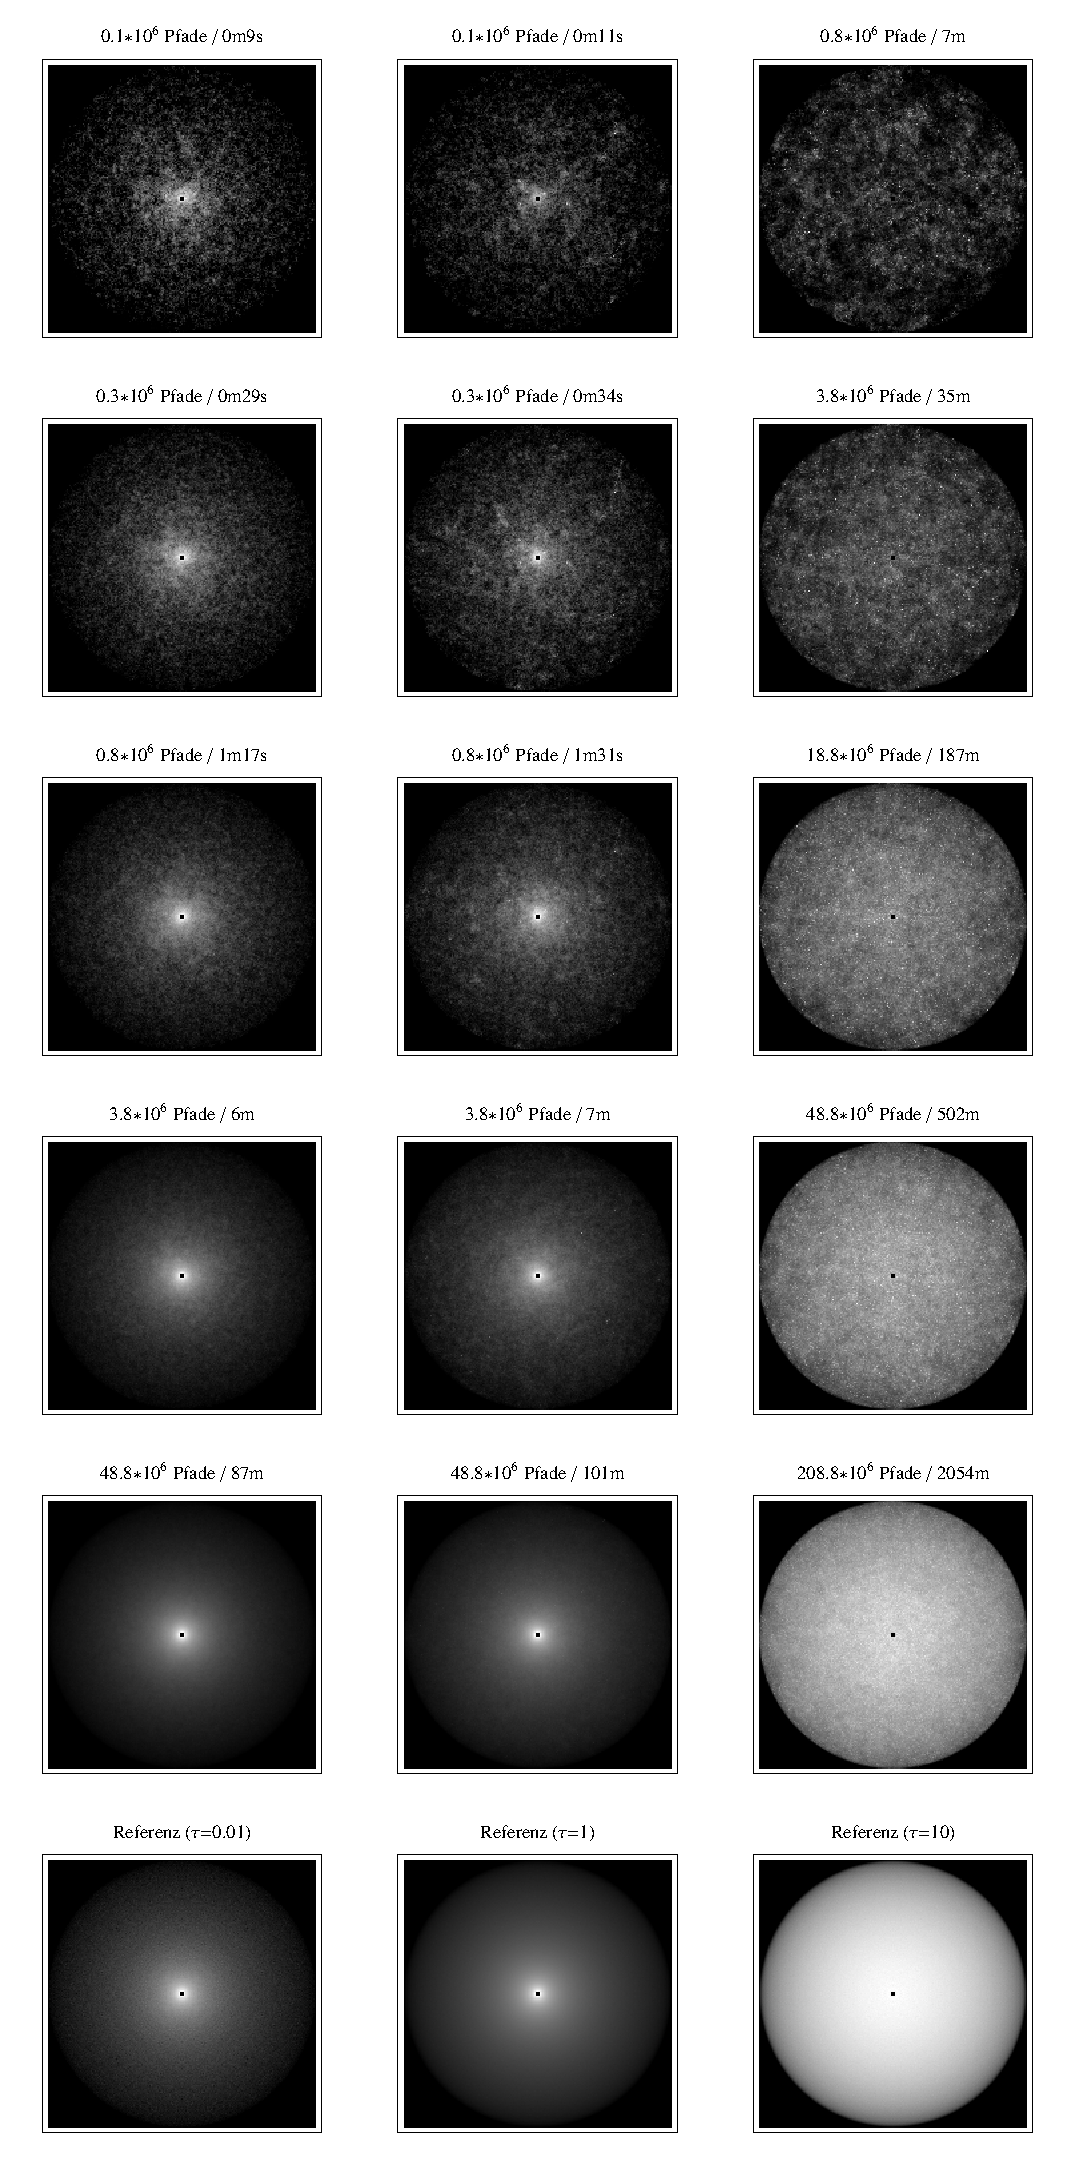
\includegraphics[height=1.0\textheight]{piratesphereimageoverview.eps}
			\caption{"Ubersicht "uber die Qualit"at der Bilder bei unterschiedlich langen \texttt{PIRaTE}--Simulationsl"aufen.}
			\label{fig:pirate_sphere_imageoverview}
		\end{figure}
	
	
	Dann ergeben sich die in Abb.~\ref{fig:sphere1_error}-\ref{fig:sphere3_error} gezeigten Ergebnisse.
	
		\begin{figure}
			\centering
			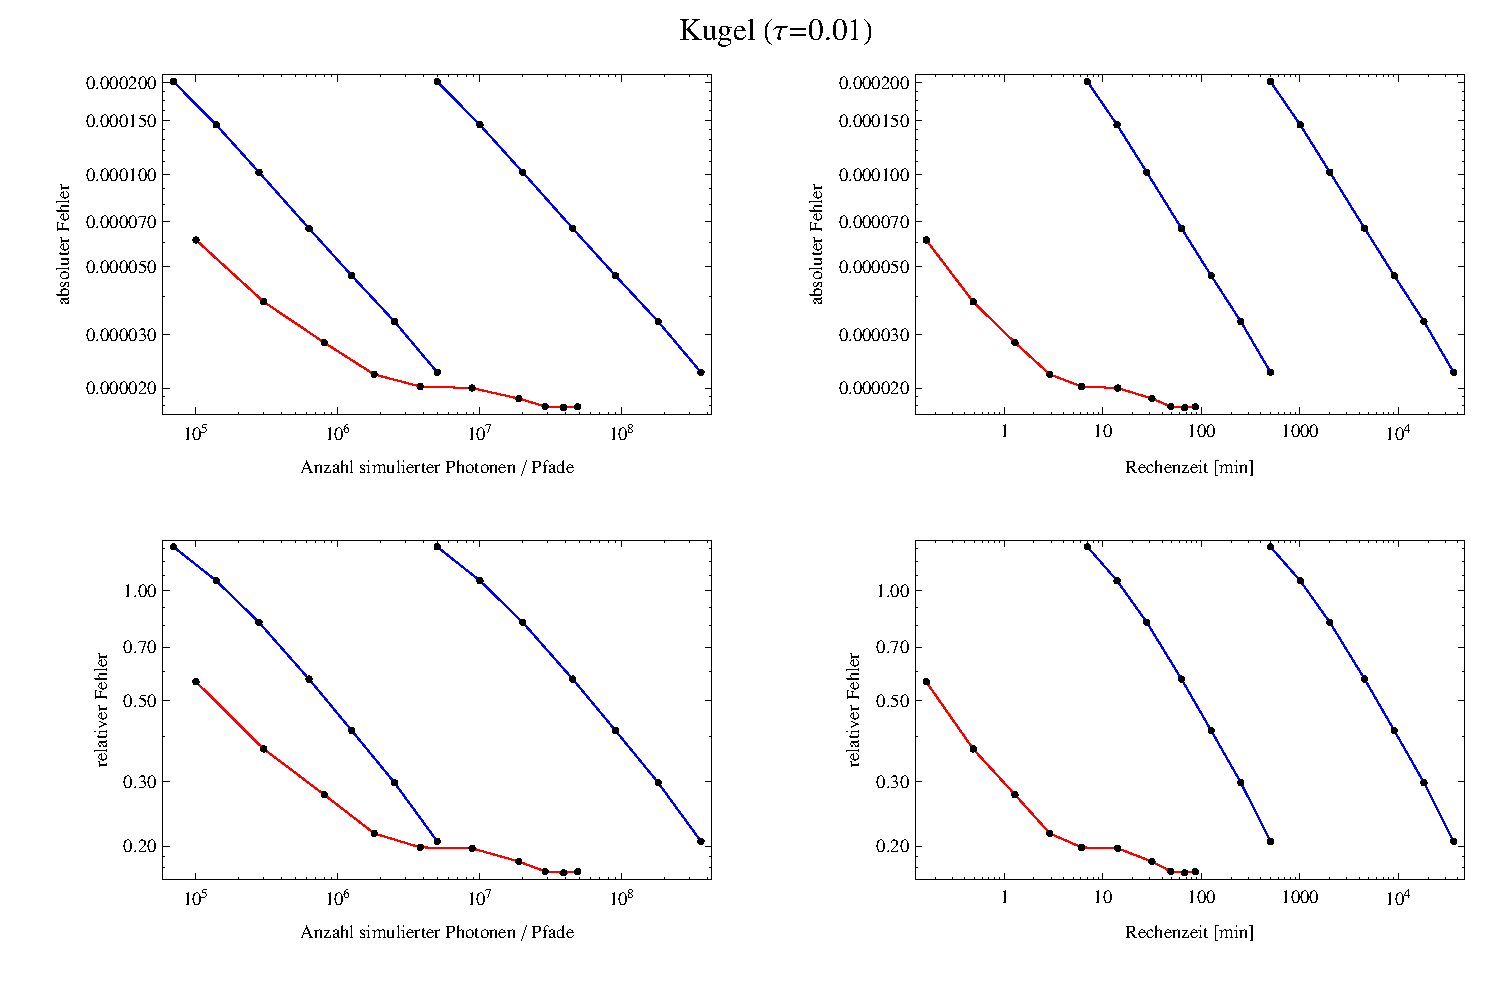
\includegraphics[angle=90,height=1.0\textheight]{sphere1errorplot.eps}
			\caption{Die blauen Linien repr"asentieren \texttt{MC3D}, wobei daf"ur die Bilder aus (1,2,4,9,18,36,72) Kameraebenen aufsummiert wurden. Die Schr"age Linie extrapoliert dabei, wie aufw"andig die Simulation mit nur einer Kameraebene gewesen w"are.}
			\label{fig:sphere1_error}
		\end{figure}
		\begin{figure}
			\centering
			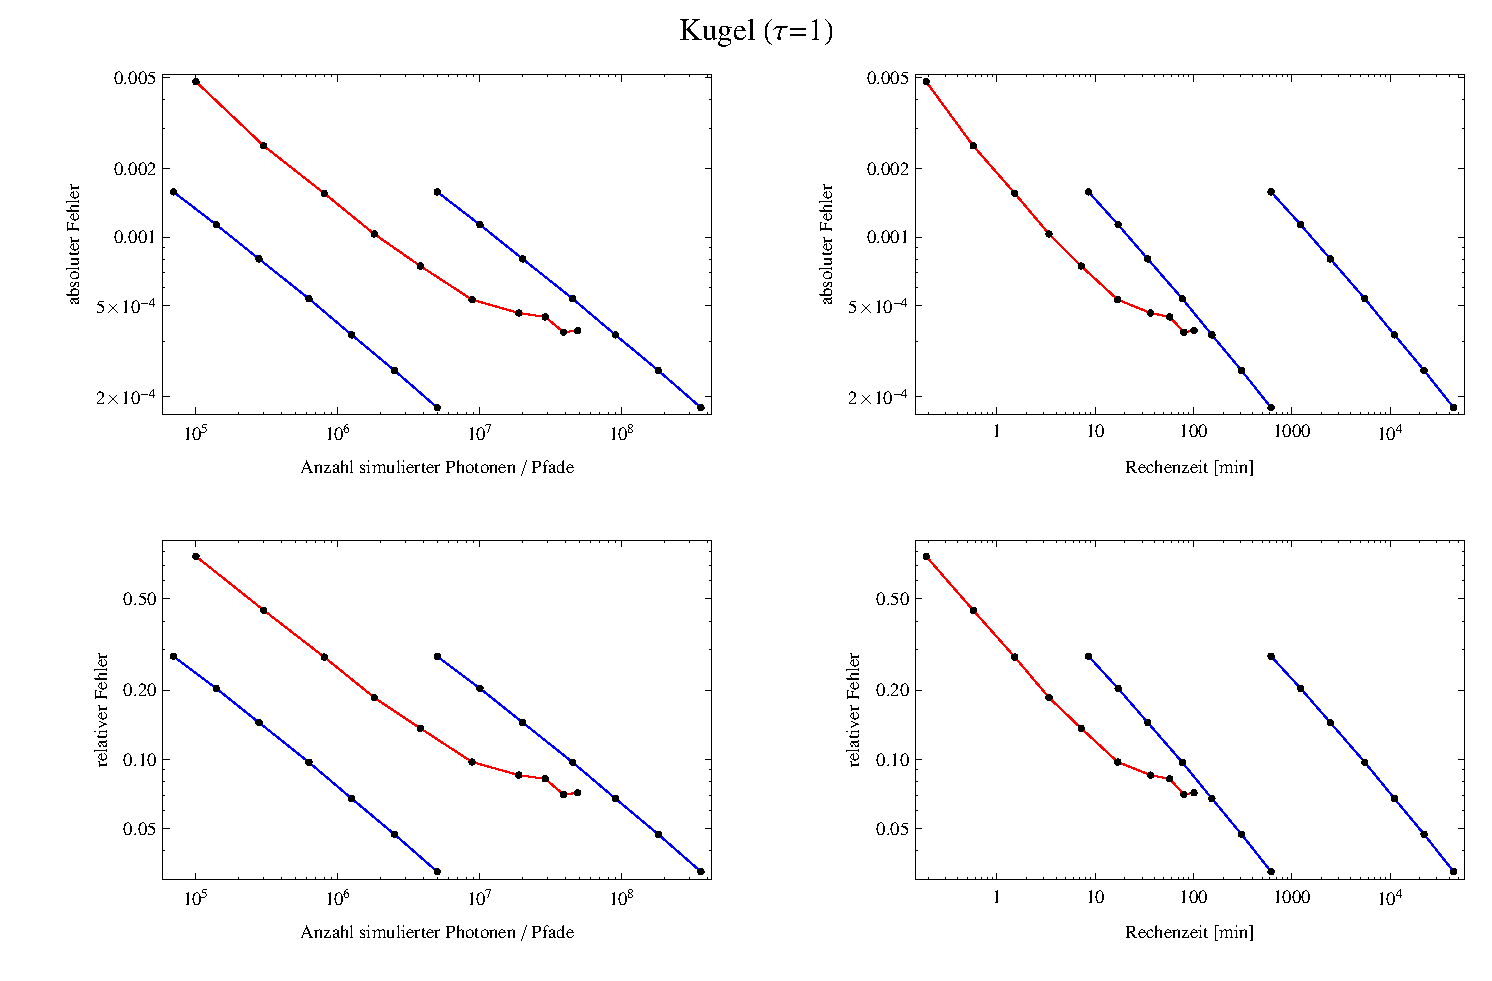
\includegraphics[angle=90,height=1.0\textheight]{sphere2errorplot.eps}
			\caption{Die blauen Linien repr"asentieren \texttt{MC3D}, wobei daf"ur die Bilder aus (1,2,4,9,18,36,72) Kameraebenen aufsummiert wurden. Die Schr"age Linie extrapoliert dabei, wie aufw"andig die Simulation mit nur einer Kameraebene gewesen w"are.}
			\label{fig:sphere2_error}
		\end{figure}
		\begin{figure}
			\centering
			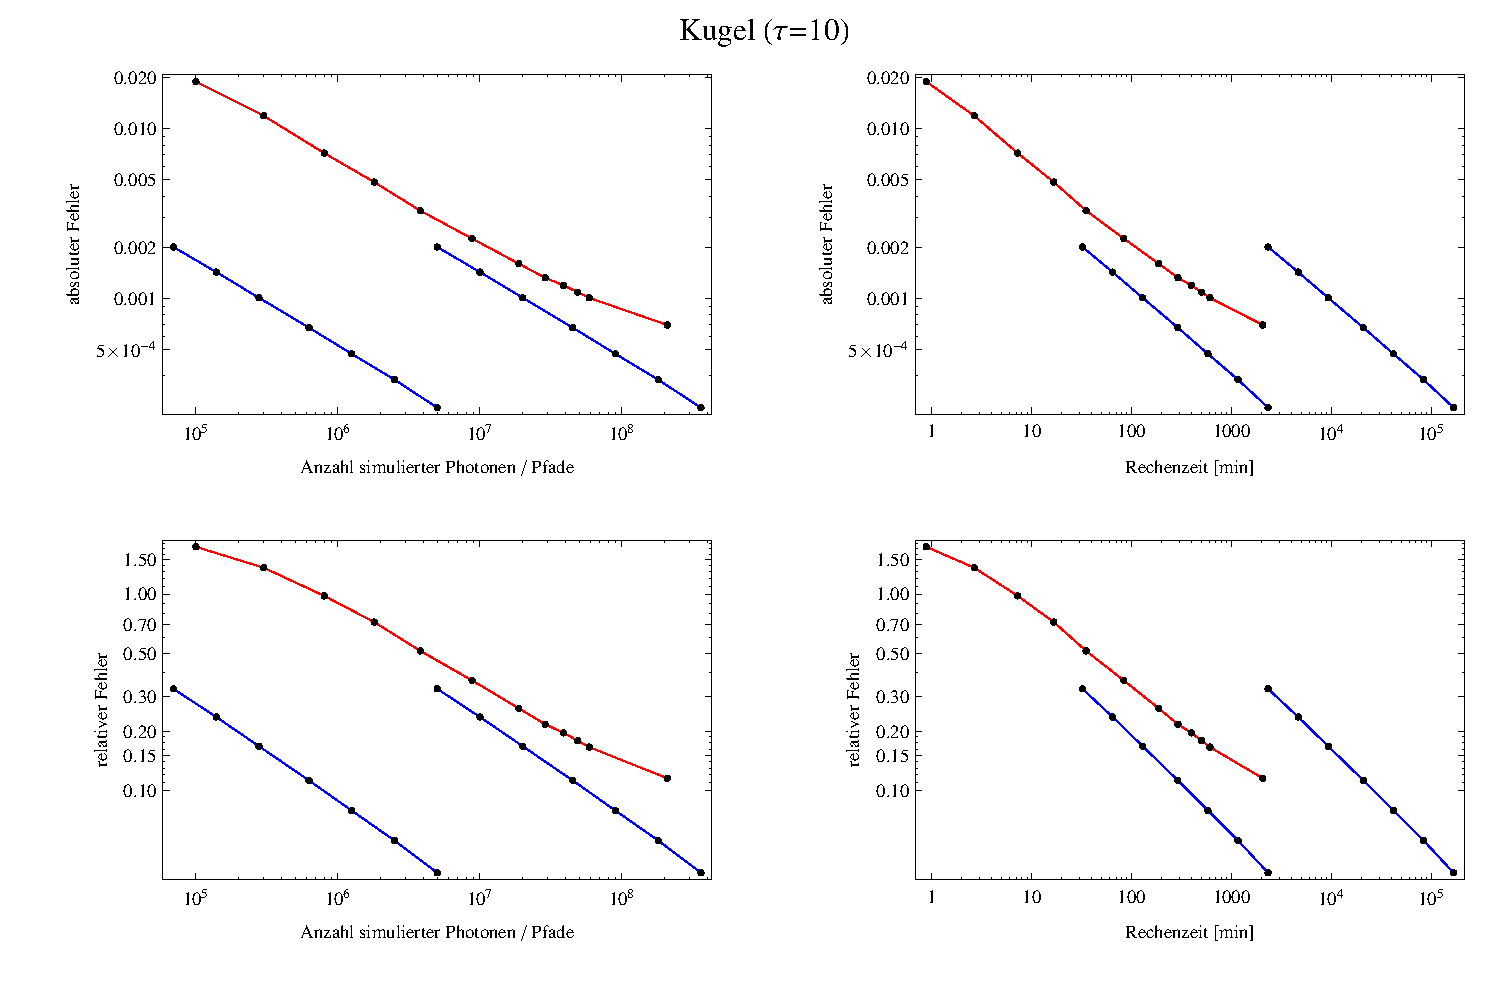
\includegraphics[angle=90,height=1.0\textheight]{sphere3errorplot.eps}
			\caption{Die blauen Linien repr"asentieren \texttt{MC3D}, wobei daf"ur die Bilder aus (1,2,4,9,18,36,72) Kameraebenen aufsummiert wurden. Die Schr"age Linie extrapoliert dabei, wie aufw"andig die Simulation mit nur einer Kameraebene gewesen w"are.}
			\label{fig:sphere3_error}
		\end{figure}
	
	\section{Einfaches Scheibenmodell}
	TODO: Formel und KonturPlot f"ur Dichteverteilung.
	\subsection{Resultate}
	TODO: Konvergenz--Geschwindigkeits--Vergleich mit MC3D.
	Stichpunkte:tau=97.6958 in der Mittelebene. 1m55s f"ur $10^6$ Photonen mit MC3D. 720M Photonen in 72Ebenen $\rightarrow$ Jede Ebene entspricht 10M Photonen
	\section{Einordnung der Resultate}
	TODO: Gesamtvergleich zwischen MC3D und PIRaTE: PIRaTE schneller, MC3D nat"urlicheres Rauschen, PIRaTE bedarf weiterer Kalibration f"ur ZentralSternIntensit"at	
	
	\chapter{Zusammenfassung und Ausblick}
	TODO: Ausblick: Normierung, physikalisch relevante Streuphasenfunktionen, polychromatische Bilder/SEDs

\backmatter
	\bibliographystyle{chicago}
	\bibliography{bibliography}

\end{document}